%\documentclass{zemplate}
\documentclass[a4paper,11pt]{article}
\usepackage{../../../Template/zemplate}
\usepackage{float}
\usepackage{multirow}
\usepackage{fixltx2e}

%\externaldocument{../Glossario/Glossario}

\includeGlossario

\docTitle{Piano di progetto}
\docVersion{4.0.0}
\docCreationDate{\frmdata{04}{12}{2016}}
\docLastUpdateDate{\frmdata{18}{08}{2017}}
\docStatus{Approvato}
\docEditors{Marco Pasqualini}
\docVerificators{Giulia Petenazzi \\ & Giovanni Prete}
\docApprovers{Marco Pasqualini}
\docUse{Esterno}
\docDestination{\Tullio \\ & \Cardin \\ & \zephyrus \\ & \riskapp}
\docJournal{
	4.0.0 & \frmdata{18}{08}{2017} & Marco Pasqualini & \responsabile & Approvazione\\
	3.1.0 & \frmdata{18}{08}{2017} & Giulia Petenazzi & \verificatore & Verifica del documento\\
	3.0.2 & \frmdata{17}{08}{2017} & Marco Pasqualini & \responsabile & Aggiunta attualizzazione del periodo Va in sezione 2, in 5.2.4 e in 5.3, 5.4, 5.5 e rimossa sezione 6. \\
	3.0.1 & \frmdata{26}{05}{2017} & Marco Pasqualini & \responsabile & Aggiunta sezione 3.2.5.\\
	%------------------------------------------------
	3.0.0 & \frmdata{07}{04}{2017} & Daniel De Gaspari & \responsabile & Approvazione\\
	2.1.0 & \frmdata{07}{04}{2017} & Leonardo Brutesco & \verificatore & Verifica del documento\\
	2.0.2 & \frmdata{06}{04}{2017} & Daniel De Gaspari & \responsabile & Aggiornata sezione 5.\\
	2.0.1 & \frmdata{06}{04}{2017} & Daniel De Gaspari & \responsabile & Aggiunta attualizzazione del periodo PCV in sezione 2, aggiornate sezione 4.2.3, 4.3, 4.4, 4.5, 4.6.\\
	%------------------------------------------------
	2.0.0 & \frmdata{03}{03}{2017} & Giovanni Damo & \responsabile & Approvazione\\
	1.2.0 & \frmdata{02}{03}{2017} & Leonardo Brutesco & \verificatore & Verificato il consuntivo di fine periodo e il preventivo a finire\\
	1.1.3 & \frmdata{02}{03}{2017} & Giovanni Damo & \responsabile & Redatto il preventivo a finire\\
	1.1.2 & \frmdata{01}{03}{2017} & Giovanni Damo & \responsabile & Redatto il consuntivo di fine periodo\\
	1.1.1 & \frmdata{10}{02}{2017} & Leonardo Brutesco & \responsabile & Corretti gli errori grammaticali nella sezione 3.1.1.1 e l'introduzione testuale del consuntivo come indicato dal verificatore\\
	1.1.0& \frmdata{10}{02}{2017} & Jordan Gottardo & \verificatore & Verifica parziale\\
	1.0.5 & \frmdata{09}{02}{2017} & Leonardo Brutesco & \responsabile & Modificati i prospetti orari della sezione Preventivo sulla base degli accorpamenti effettuati nella sezione di pianificazione.\\
	1.0.4 & \frmdata{08}{02}{2017} & Leonardo Brutesco & \responsabile & Ristrutturata la pianificazione secondo le osservazioni dei docenti, al fine di rendere chiaro che il modello scelto è quello incrementale. Rimasta invariata la pianificazione dei primi due periodi; raggruppate quelle che prima erano le fasi PdROb, PdRD, PdROp nell'unico periodo PCV caratterizzato da vari incrementi, definiti all'inizio del secondo periodo. Nei diagrammi di Gantt sono stati introdotti i task per le attività di Analisi dei Requisiti e di Progettazione logica.\\
	1.0.3 & \frmdata{07}{02}{2017} & Leonardo Brutesco & \responsabile & Trasposta l'analisi dei rischi in forma tabellare nella sezione 2\\
	1.0.2 & \frmdata{06}{02}{2017} & Leonardo Brutesco & \responsabile & Sostituita la parola "fase" con "periodo".\\
	1.0.1 & \frmdata{29}{01}{2017} & Giovanni Damo & \responsabile & Messi a glossario i termini solo la prima volta che compaiono in ogni section del documento \\
	%------------------------------------------------
	1.0.0 & \frmdata{07}{01}{2017} & Giulia Petenazzi & \responsabile & Approvazione \\
	0.2.0 & \frmdata{07}{01}{2017} & Daniel De Gaspari & \verificatore & Verifica del documento\\
	0.1.3 & \frmdata{06}{01}{2017} & Giulia Petenazzi & \responsabile & Stesura preventivo a finire\\
	0.1.2 & \frmdata{05}{01}{2017} & Giulia Petenazzi & \responsabile & Stesura consuntivo di periodo\\
	0.1.1 & \frmdata{05}{01}{2017} & Giulia Petenazzi & \responsabile & Correzione errori\\
	0.1.0 & \frmdata{14}{12}{2016} & Marco Pasqualini & \verificatore & Verifica parziale\\
	0.0.6 & \frmdata{12}{12}{2016} & Giulia Petenazzi & \responsabile & Stesura preventivo \\
	0.0.5 & \frmdata{07}{12}{2016} & Jordan Gottardo & \responsabile & Stesura organigramma \\
	0.0.4 & \frmdata{06}{12}{2016} & Jordan Gottardo & \responsabile & Stesura pianificazione \\
	0.0.3 & \frmdata{05}{12}{2016} & Giulia Petenazzi & \responsabile & Stesura analisi dei rischi \\
	0.0.2 & \frmdata{05}{12}{2016} & Jordan Gottardo & \responsabile & Stesura introduzione \\
	0.0.1 & \frmdata{04}{12}{2016} & Jordan Gottardo & \responsabile & Creazione template e indice \\
}
\usepackage{multirow}
\usepackage{float}

\begin{document}
	% section {Introduzione}
\section {Introduzione}
	\subsection {Scopo del documento}
	Con il seguente documento si intende pianificare il modo e i tempi in cui il \glo{Gruppo}{gruppo} intende sviluppare il progetto \progetto. In particolare, gli scopi del documento sono:
	\begin{itemize}
	 \item {analizzare e gestire i fattori di rischio;}
	 \item {collocare le attività da svolgere nel tempo;}
	 \item {assegnare le attività da svolgere ai membri del gruppo;}
	 \item {definire il preventivo dei costi;}
	 \item {definire il consuntivo di periodo;}
	 \item {definire il preventivo a finire.}
	\end{itemize}
	\subsection {Scopo del prodotto}
	\introScopo
	\subsection {Glossario}
	\introGlossario
	\subsection {Riferimenti}
		\subsubsection{Riferimenti normativi}
		\begin{itemize}
				\item \textbf{regole del progetto didattico:}\\
                \url{http://www.math.unipd.it/~tullio/IS-1/2016/Dispense/L09.pdf};
				\item {\ndpv};
				\item \textbf{\glo{Capitolato}{capitolato} d'appalto:}\\
                \url{http://www.math.unipd.it/~tullio/IS-1/2016/Progetto/C3.pdf}
		\end{itemize}
		\subsubsection{Riferimenti informativi}
		\begin{itemize}
				\item \textbf{slides del corso di Ingegneria del Software:}\\
                \url{http://www.math.unipd.it/~tullio/IS-1/2016/};
                \item \textbf{SWEBok - Chapter 8:Software Engineering Management:}\\
                \url{http://www.math.unipd.it/~tullio/IS-1/2007/Approfondimenti/SWEBOK.pdf};
				\item {\sdfv};
				\item {\pdqv};
				\item {\adrv};
				\item \textbf{regolamento di Organigramma:}
				\url{http://www.math.unipd.it/~tullio/IS-1/2016/Progetto/PD01b.html}.
		\end{itemize}
	\subsection {Scadenze e altri vincoli}
	\label{subsec:scadenze}
	\begin{itemize}
	\item
		È stato deciso di rispettare le seguenti scadenze di consegna del materiale:
		\begin{itemize}
			 \item {\revereq}: \frmdata{11}{01}{2017};
			 \item {\revprog}: \frmdata{06}{03}{2017};
			 \item {\revaqual}: \frmdata{11}{04}{2017};
			 \item {\revacc}: \frmdata{08}{05}{2017}.
		\end{itemize}
	\item
		Ogni componente del gruppo deve dimostrare di aver impiegato, per lo svolgimento del progetto, un numero di ore maggiore (o pari) a 85 e inferiore (o pari) a 105.
		Un componente del gruppo, Giovanni Damo, dovrà lasciare lo svolgimento del progetto in data \frmdata{11}{04}{2017}. All'uscita dal progetto il componente dovrà aver comunque adempiuto all'obbligo sopra descritto.
	\end{itemize}
	%subsection {Scelta RP min/max} io la metterei nella pianificazione

	%\section {Analisi dei rischi}
\section {Analisi dei rischi}
\label{sec:analisirischi}
	\subsection {Introduzione}
	In questa sezione vengono descritti i rischi che potrebbero verificarsi durante lo svolgimento del progetto.
	I rischi possono essere a livello:
	\begin{itemize}
	 \item {tecnologico};
	 \item {personale};
	 \item {organizzativo};
	 \item {dei requisiti}.
	\end{itemize}
	Per ogni rischio deve essere indicato:
	 \begin{itemize}
	 \item {nome};
	 \item {descrizione};
	 \item {possibili conseguenze};
	 \item {analisi}:
	 	\begin{itemize}
	 	\item \textbf{probabilità di occorrenza}: (alta/media/bassa) mostra una stima preventiva della probabilità che il rischio si verifichi senza aver attuato alcuna misura di prevenzione;
	 	\item \textbf{impatto}: (alto/medio/basso) mostra una stima preventiva dell'impatto del rischio, nel caso in cui si verificasse senza aver deciso di attuare alcuna procedura di contenimento.
	 	\end{itemize}
	 \item \textbf{{prevenzione}:} spiega come si è deciso di prevenire il verificarsi del rischio;
	 \item \textbf{{identificazione}:} mostra come il \glo{Gruppo}{gruppo} riuscirà a capire che il rischio si sta verificando e come verrà attivata la procedura di contenimento;
	 \item \textbf{{contenimento}:} spiega come si è deciso di contenere le conseguenze del rischio una volta verificato. Oltre alle misure descritte successivamente per ogni specifico rischio, si è deciso di inserire dei tempi di \glo{Slack}{slack} nel piano di lavoro, sfruttabili nel caso in cui il \responsabilediprogetto{} lo ritenesse necessario al verificarsi dei rischi;
	 \item \textbf{{analisi mitigata}:}
	 \begin{itemize}
	 	\item \textbf{probabilità mitigata di occorrenza}: (alta/media/bassa) mostra una stima preventiva della probabilità che il rischio si verifichi dopo aver attuato le opportune misure di prevenzione sopra descritte;
	 	\item \textbf{impatto mitigato}: (alto/medio/basso) mostra una stima preventiva dell'impatto del rischio, nel caso in cui si verificasse, decidendo di attuare le opportune misure di contenimento sopra descritte.
	 \end{itemize}

	 \item \textbf{{attualizzazione nel periodo}:} viene descritto se il rischio si è verificato, le reazioni del gruppo e le conseguenze effettivamente prodotte.
	 \\Per le sigle relative ai periodi si veda: \ref{Pdrob-ProcessiAttività}.
	 \end{itemize}
	 
	


	\subsection {Panoramica generale}
	Viene mostrata una tabella che illustra i rischi individuati, la loro probabilità mitigata di occorrenza, il loro impatto mitigato.
	\begin{table}[H]
	\begin{center}
	\small
		\begin{tabular}{lllll}
			\toprule
				Livello & Rif. & Rischio & Probabilità & Impatto \\
			\midrule
				\multirow{3}{*}{Tecnologico}
				& (\ref{subsec:malfunzionamenttiSwHw})
				& Malfunzionamenti software e hardware
				& Bassa & Basso \\
				& (\ref{subsec:difficoltaTecnol})
				& Difficoltà nell'uso delle tecnologie
				& Media & Medio \\
				& (\ref{subsec:indisponibilitaTablet})
				& Indisponibilità tablet
				& Media & Basso \\
			\midrule
				\multirow{3}{*}{Personale}
				& (\ref{subsec:pbmDeiMembri})
				& Problemi dei membri
				& Media & Medio \\
				& (\ref{subsec:pbmTraMembri})
				& Problemi tra i membri
				& Bassa & Medio\\
				& (\ref{subsec:pbmProponente})
				& Problemi con il proponente
				& Bassa & Medio \\
			\midrule
				Organizzativo & (\ref{subsec:errataPianificazione})
				& Errata pianificazione dell'uso delle risorse
				& Bassa & Medio \\
			\midrule
				Dei Requisiti & (\ref{subsec:erratiRequisiti})
				& Errata o incompleta analisi dei requisiti
				& Bassa & Medio \\
			\bottomrule
			\end{tabular}
		\end{center}
		\caption{Rischi individuati}
		\label{tab:rischi}
	\end{table}
	
	\newpage
	\subsection {Livello tecnologico}
		\subsubsection {Malfunzionamenti software e hardware}
			\label{subsec:malfunzionamenttiSwHw}
			\small
			\begin{table}[H]
			\begin{center}			
			\begin{tabular}{p{2.5cm}p{0.5cm}p{11cm}}
			\arrayrulecolor{lightgray}
			
			\toprule				
				\textbf{Descrizione}
				& &
				Ogni membro del gruppo userà i propri dispositivi (computer, smartphone, tablet).
				Non si escludono rotture o danneggiamenti di tali dispositivi, malfunzionamenti dei software necessari allo svolgimento del progetto o problemi di compatibilità.
			\\
			\midrule
				\textbf{Possibili \newline conseguenze}
				& &
				Ritardi nei lavori, perdita dei dati.
			\\
			\midrule
				\textbf{Prevenzione}
				& &
	 			I membri del gruppo eseguiranno backup regolari nel \glo{Repository}{repository}.
	 		\\
			\midrule
				\textbf{Identificazione}
				& &
				I membri del gruppo dovranno controllare periodicamente i propri dispositivi, i software utilizzati ed i dati prodotti. In caso di malfunzionamenti avviseranno il \responsabilediprogetto.
			\\
			\midrule
				\textbf{Contenimento}
				& &
				Il \responsabilediprogetto, dopo essersi consultato con i membri che hanno riscontrato il malfunzionamento, potrà eventualmente decidere di alleggerire o modificare il loro carico di lavoro. Eventuali dati persi a causa del malfunzionamento dovranno, se possibile, essere ripristinati dal repository. In caso di necessità si potranno usare i computer dei laboratori, messi a disposizione dall'università, per la continuazione del lavoro.
			\\
			\midrule
				\textbf{Analisi \newline non mitigata}
				& &
				\textbf{Probabilità di occorrenza}: Bassa
				\newline
				\textbf{Impatto}: Alto
			\\
			\midrule
				\textbf{Analisi \newline mitigata}
				& &
				\textbf{Probabilità di occorrenza}: Bassa
				\newline
				\textbf{Impatto}: Basso
			\\
			\midrule
				\textbf{Attualizzazione}
				& &
				\textbf{An}: Il rischio non si è verificato.
				\newline
				\textbf{Pl}: Il rischio non si è verificato.
			\\
			
			\bottomrule	
			\end{tabular}
			\end{center}
			\end{table}			
			
	\newpage
		\subsubsection {Difficoltà nell'uso delle tecnologie}
		\label{subsec:difficoltaTecnol}
		
		
					\small
					\begin{table}[H]
					\begin{center}			
					\begin{tabular}{p{2.5cm}p{0.5cm}p{11cm}}
					\arrayrulecolor{lightgray}
					
					\toprule				
						\textbf{Descrizione}
						& &
						Per lo svolgimento del progetto sarà necessario utilizzare tecnologie con le quali non tutti i membri del gruppo hanno esperienza. Potrebbero quindi sorgere difficoltà nell'utilizzo di queste tecnologie.
					\\
					\midrule
						\textbf{Possibili \newline conseguenze}
						& &
						Ritardi nei lavori.
					\\
					\midrule
						\textbf{Prevenzione}
						& &
						Le tecnologie da usare verrano decise con congruo anticipo. Saranno previsti nel piano di lavoro momenti di formazione. Gli \amministratori{} forniranno la documentazione e i riferimenti necessari allo studio autonomo delle tecnologie.
					\\
					\midrule
						\textbf{Identificazione}
						& &
						Sarà compito del \responsabilediprogetto{} e degli \amministratori{} verificare il grado di conoscenza delle tecnologie richieste. I membri del gruppo che dovessero trovare difficoltà nell'uso delle tecnologie richieste durante lo svolgimento dovranno avvisare il \responsabilediprogetto.
					\\
					\midrule
						\textbf{Contenimento}
						& &
						Il \responsabilediprogetto{} potrà sollevare momentaneamente il membro carente dal proprio incarico. Il piano di lavoro potrà essere variato per permettere al membro carente di aggiornarsi nel minor tempo possibile. Nel caso in cui il membro non riesca a utilizzare la tecnologia allora dovrà essere sostituito. Se possibile la tecnologia potrà essere sostituita da una tecnologia equivalente.
					\\
					\midrule
						\textbf{Analisi \newline non mitigata}
						& &
						\textbf{Probabilità di occorrenza}: Alta
						\newline
						\textbf{Impatto}: Alto
					\\
					\midrule
						\textbf{Analisi \newline mitigata}
						& &
						\textbf{Probabilità di occorrenza}: Media
						\newline
						\textbf{Impatto}: Medio
					\\
					\midrule
						\textbf{Attualizzazione}
						& &
						\textbf{An}: Lo strumento di gestione di progetto scelto inzialmente si è dimostrato poco flessibile, carente di alcune funzionalità e poco integrato negli smartphone. Il \responsabilediprogetto{} e gli \amministratori{} hanno deciso di sostituire lo strumento con un altro più completo e maggiormente integrato. Ci sono stati inoltre problemi con il software di tracciamento dei requisiti. Il \responsabilediprogetto, dopo aver provato a modificare lo strumento, ha deciso di sostituirlo con uno equivalente.
						\newline
						\textbf{Pl}: Il rischio non si è verificato.
					\\
					
					\bottomrule	
					\end{tabular}
					\end{center}
					\end{table}			

	\newpage
		\subsubsection{Indisponibilità tablet}
		\label{subsec:indisponibilitaTablet}
		
		
					\small
					\begin{table}[H]
					\begin{center}			
					\begin{tabular}{p{2.5cm}p{0.5cm}p{11cm}}
					\arrayrulecolor{lightgray}
					
					\toprule				
						\textbf{Descrizione}
						& &
						Il progetto richiede lo sviluppo di un'interfaccia utilizzabile da tablet. Specialmente per quanto riguarda l'attività di testing sarà quindi necessario avere almeno un tablet a disposizione su cui testare il funzionamento dell'applicazione. Due membri sono dotati di tablet personale, ma è da prendere in considerazione il caso in cui non ci sia la possibilità di averli a disposizione.
					\\
					\midrule
						\textbf{Possibili \newline conseguenze}
						& &
						Ritardi nei lavori.
					\\
					\midrule
						\textbf{Prevenzione}
						& &
						I due membri del gruppo comunicano al \responsabilediprogetto{} i giorni in cui offrono la disponibilità del tablet.
					\\
					\midrule
						\textbf{Identificazione}
						& &
						Nel caso in cui i due membri del gruppo non possano mettere a disposizione il tablet nei giorni stabiliti, informeranno preventivamente il \responsabilediprogetto{}.
					\\
					\midrule
						\textbf{Contenimento}
						& &
						Il \responsabilediprogetto{} comunicherà il problema agli altri membri del gruppo che dovranno quindi eseguire i test su smartphone o strumenti equivalenti.
					\\
					\midrule
						\textbf{Analisi \newline non mitigata}
						& &
						\textbf{Probabilità di occorrenza}: Alta
						\newline
						\textbf{Impatto}: Medio
					\\
					\midrule
						\textbf{Analisi \newline mitigata}
						& &
						\textbf{Probabilità di occorrenza}: Media
						\newline
						\textbf{Impatto}: Basso
					\\
					\midrule
						\textbf{Attualizzazione}
						& &
						\textbf{An}: Il rischio non si è verificato.
						\newline
						\textbf{Pl}: Il rischio non si è verificato.
					\\
					
					\bottomrule	
					\end{tabular}
					\end{center}
					\end{table}			
	
	\subsection {Livello personale}
		\subsubsection {Problemi dei membri}
		\label{subsec:pbmDeiMembri}
		
		
					\begin{table}[H]
					\begin{center}
					\resizebox{0.98\textwidth}{!}{
					\begin{tabular}{p{2.5cm}p{0.5cm}p{11cm}}
					\arrayrulecolor{lightgray}
					
					\toprule				
						\textbf{Descrizione}
						& &
						 Gli impegni personali e universitari dei singoli membri possono far sì che non sempre questi siano disponibili a lavorare sul progetto o a presenziare alle riunioni.
					\\
					\midrule
						\textbf{Possibili \newline conseguenze}
						& &
						Ritardi nei lavori.
					\\
					\midrule
						\textbf{Prevenzione}
						& &
						Viene predisposto un orario settimanale condiviso su cui segnare gli impegni ricorrenti dei membri del gruppo per facilitare l'organizzazione delle riunioni. Il \responsabilediprogetto{} dovrà scegliere per le riunioni i giorni e gli orari con il maggior numero di presenze. Durante la pianificazione del lavoro si dovrà tener conto dei periodi di maggiore indisponibilità dei membri come, ad esempio, sessioni d'esame.
					\\
					\midrule
						\textbf{Identificazione}
						& &
						In caso di imprevisti i membri del gruppo dovranno informare in maniera tempestiva il \responsabilediprogetto{} sfruttando gli strumenti di comunicazione messi a disposizione.
					\\
					\midrule
						\textbf{Contenimento}
						& &
						In caso si tratti di imprevisti sulla partecipazione ad una riunione, il \responsabilediprogetto{} potrà decidere di spostare la riunione. Al termine di ogni riunione viene stilato un verbale di cui il membro mancante potrà prendere visione. In caso si tratti di imprevisti sul lavoro da svolgere, il \responsabilediprogetto{} potrà provvedere a modificare la pianificazione e se necessario, riassegnare il lavoro.
					\\
					\midrule
						\textbf{Analisi \newline non mitigata}
						& &
						\textbf{Probabilità di occorrenza}: Alta
						\newline
						\textbf{Impatto}: Alto
					\\
					\midrule
						\textbf{Analisi \newline mitigata}
						& &
						\textbf{Probabilità di occorrenza}: Media
						\newline
						\textbf{Impatto}: Medio
					\\
					\midrule
						\textbf{Attualizzazione}
						& &
						\textbf{An}: Il rischio si è in parte verificato in quanto un membro del gruppo, essendo impegnato in attività di stage, non ha potuto partecipare ad alcune riunioni. Il membro si è tenuto aggiornato con le decisioni prese attraverso i canali di comunicazione e prendendo visione di tutti i verbali.
						\newline
						\textbf{Pl}: Il rischio si è verificato per due motivi.
						- Innanzitutto un membro del gruppo ha avuto gravi problemi di salute durante la seconda parte del mese di Febbraio. Il membro, non appena è venuto a conoscenza del problema, ossia verso inizio mese, ha informato tempestivamente il \responsabile. Quest'ultimo (come descritto da questa analisi nella sezione "Contenimento") ha riorganizzato la pianificazione al fine di anticipare le ore di lavoro del membro colpito alla prima parte di Febbraio. Questi cambiamenti 
						rispetto al preventivo sono evidenziati in tabella \ref{tab:orePl}. In questo modo l'impatto dato dal verificarsi di questo rischio è stato ben attutito.
						- In secondo luogo, a causa della sessione esami, alcuni membri hanno lavorato poco nei momenti iniziali di questo periodo di Progettazione logica. Questo rischio era stato preventivato, e la pianificazione teneva già conto di questa impossibilità, pertanto il rischio non ha avuto un grosso impatto.
					\\
					
					\bottomrule	
					\end{tabular}}
					\end{center}
					\end{table}			
				\newpage

		\subsubsection {Problemi tra i membri}
		\label{subsec:pbmTraMembri}
		
					\small
					\begin{table}[H]
					\begin{center}			
					\begin{tabular}{p{2.5cm}p{0.5cm}p{11cm}}
					\arrayrulecolor{lightgray}
					
					\toprule				
						\textbf{Descrizione}
						& &
						I membri del gruppo non hanno mai lavorato ad un progetto di gruppo di così grandi dimensioni. Potrebbero verificarsi contrasti tra i membri del gruppo, e quindi problemi di collaborazione.
					\\
					\midrule
						\textbf{Possibili \newline conseguenze}
						& &
						Ambiente non adatto al lavoro cooperativo, ritardi nei lavori.
					\\
					\midrule
						\textbf{Prevenzione}
						& &
						 I membri del \glo{Gruppo}{team} cercheranno di fornire critiche solo se costruttive.
					\\
					\midrule
						\textbf{Identificazione}
						& &
						Ogni membro del gruppo comunicherà al \responsabilediprogetto{} eventuali dissapori al fine di risolvere al più presto eventuali situazioni problematiche.
					\\
					\midrule
						\textbf{Contenimento}
						& &
						Il \responsabilediprogetto{} dovrà capire il problema e appianare le divergenze. Se necessario potrà provvedere alla riorganizzazione del piano di lavoro separando i membri coinvolti.
					\\
					\midrule
						\textbf{Analisi \newline non mitigata}
						& &
						\textbf{Probabilità di occorrenza}: Bassa
						\newline
						\textbf{Impatto}: Alto
					\\
					\midrule
						\textbf{Analisi \newline mitigata}
						& &
						\textbf{Probabilità di occorrenza}: Bassa
						\newline
						\textbf{Impatto}: Medio
					\\
					\midrule
						\textbf{Attualizzazione}
						& &
						\textbf{An}: Il rischio non si è verificato.
						\newline
						\textbf{Pl}: Il rischio non si è verificato.
					\\
					
					\bottomrule	
					\end{tabular}
					\end{center}
					\end{table}			

	\newpage
		\subsubsection {Problemi col proponente}
		\label{subsec:pbmProponente}
		
		
					\small
					\begin{table}[H]
					\begin{center}			
					\begin{tabular}{p{2.5cm}p{0.5cm}p{11cm}}
					\arrayrulecolor{lightgray}
					
					\toprule				
						\textbf{Descrizione}
						& &
						Potrebbero verificarsi ritardi da parte del proponente nelle comunicazioni o nel fornire il materiale richiesto.
					\\
					\midrule
						\textbf{Possibili \newline conseguenze}
						& &
						Ritardi nei lavori.
					\\
					\midrule
						\textbf{Prevenzione}
						& &
						Le scadenze a cui è soggetto il gruppo saranno rese note al proponente al fine di migliorare le tempistiche di collaborazione.
					\\
					\midrule
						\textbf{Identificazione}
						& &
						Nel caso in cui non si ottenessero le risposte o il materiale atteso entro una settimana dalle richieste, il \responsabilediprogetto{} provvederà ad inviare un sollecito.
					\\
					\midrule
						\textbf{Contenimento}
						& &
						 Il \responsabilediprogetto{} potrà valutare se riorganizzare il piano di lavoro per procedere con l'esecuzione di altri lavori non dipendenti dalle risposte del proponente.
					\\
					\midrule
						\textbf{Analisi \newline non mitigata}
						& &
						\textbf{Probabilità di occorrenza}: Media
						\newline
						\textbf{Impatto}: Alto
					\\
					\midrule
						\textbf{Analisi \newline mitigata}
						& &
						\textbf{Probabilità di occorrenza}: Bassa
						\newline
						\textbf{Impatto}: Medio
					\\
					\midrule
						\textbf{Attualizzazione}
						& &
						\textbf{An}: Il rischio si è in parte verificato in quanto il proponente non ha sempre risposto prontamente alle e-mail. Inoltre parte del materiale richiesto è pervenuto tre giorni dopo rispetto a quanto previsto.
						\newline
						\textbf{Pl}: Il rischio non si è verificato.
					\\
					
					\bottomrule	
					\end{tabular}
					\end{center}
					\end{table}			
	
				
	\newpage
	\subsection{Livello organizzativo}
		\subsubsection {Errata pianificazione di uso delle risorse}
			\label{subsec:errataPianificazione}
			
						\small
						\begin{table}[H]
						\begin{center}			
						\begin{tabular}{p{2.5cm}p{0.5cm}p{11cm}}
						\arrayrulecolor{lightgray}
						
						\toprule				
							\textbf{Descrizione}
							& &
							È possibile che le stime dei tempi e dei costi siano troppo ottimistiche.
						\\
						\midrule
							\textbf{Possibili \newline conseguenze}
							& &
							Ritardi nella consegna, aumento del costo preventivato.
						\\
						\midrule
							\textbf{Prevenzione}
							& &
							La pianificazione iniziale dovrà essere essere eseguita con particolare attenzione e sottoposta a più verifiche per assicurare che non sia troppo ottimistica. I membri del gruppo dovranno utilizzare sistemi di rendicontazione del tempo di lavoro per assicurare il rispetto dei tempi previsti.
						\\
						\midrule
							\textbf{Identificazione}
							& &
							 Dovranno essere utilizzati sistemi automatici che permettano al \responsabilediprogetto{} di controllare in maniera rapida ed efficiente lo stato dei lavori.
						\\
						\midrule
							\textbf{Contenimento}
							& &
							Il \responsabilediprogetto{} potrà modificare il piano di lavoro al fine di recuperare il ritardo. Nel caso in cui il ritardo accumulato sia eccessivo si dovrà valutare col proponente di ritrattare la scadenza.
						\\
						\midrule
							\textbf{Analisi \newline non mitigata}
							& &
							\textbf{Probabilità di occorrenza}: Media
							\newline
							\textbf{Impatto}: Alto
						\\
						\midrule
							\textbf{Analisi \newline mitigata}
							& &
							\textbf{Probabilità di occorrenza}: Bassa
							\newline
							\textbf{Impatto}: Medio
						\\
						\midrule
							\textbf{Attualizzazione}
							& &
							\textbf{An}:  Il rischio non si è verificato.
							\newline
							\textbf{Pl}: Il rischio non si è verificato.
						\\
						
						\bottomrule	
						\end{tabular}
						\end{center}
						\end{table}			
						
	\newpage
	\subsection {Livello dei requisiti}
		\subsubsection {Errata o incompleta analisi dei requisiti}
			\label{subsec:erratiRequisiti}
			
						\small
						\begin{table}[H]
						\begin{center}			
						\begin{tabular}{p{2.5cm}p{0.5cm}p{11cm}}
						\arrayrulecolor{lightgray}
						
						\toprule				
							\textbf{Descrizione}
							& &
							È possibile che i requisiti individuati non rispecchino in maniera completa ed esaustiva le richieste del proponente.
						\\
						\midrule
							\textbf{Possibili \newline conseguenze}
							& &
							Ritardi nei lavori.
						\\
						\midrule
							\textbf{Prevenzione}
							& &
							Saranno organizzate riunioni con il proponente durante le quali il gruppo potrà mostrare il lavoro svolto, ricevere eventuali feedback e porre domande. Verrà inoltre predisposta una chat condivisa con il proponente che potrà essere utilizzata per chiarire eventuali dubbi in maniera più immediata rispetto all'email o alle riunioni.
						\\
						\midrule
							\textbf{Identificazione}
							& &
							Durante l'intera durata del progetto ogni membro del gruppo dovrà porre particolare attenzione alle richieste del proponente. Qualsiasi dubbio sulle richieste dovrà essere esposto al \responsabilediprogetto.
						\\
						\midrule
							\textbf{Contenimento}
							& &
							Nel caso in cui il rischio si verificasse dovrà essere fatto il possibile per riadattarsi alle esigenze del proponente. Il \responsabilediprogetto{} potrà valutare a seconda dei casi se rinegoziare i requisiti con il proponente.
						\\
						\midrule
							\textbf{Analisi \newline non mitigata}
							& &
							\textbf{Probabilità di occorrenza}: Media
							\newline
							\textbf{Impatto}: Alto
						\\
						\midrule
							\textbf{Analisi \newline mitigata}
							& &
							\textbf{Probabilità di occorrenza}: Bassa
							\newline
							\textbf{Impatto}: Medio
						\\
						\midrule
							\textbf{Attualizzazione}
							& &
							\textbf{An}: Il rischio non si è verificato.
							\newline
							\textbf{Pl}: Il rischio non si è verificato.
						\\
						
						\bottomrule	
						\end{tabular}
						\end{center}
						\end{table}			
			
	%\section {Pianificazione}
\section {Pianificazione}
\subsection {Introduzione}
	\subsubsection{Scelta modello di sviluppo}
	Il modello di \glo{Ciclo di vita}{ciclo di vita} scelto per il prodotto è il modello incrementale.\\
	Lo sviluppo del progetto viene suddiviso in quattro periodi significativi, descritti nella sezione \ref{periodi_e_milestones}.
	\paragraph{Strutturazione}
	Questo modello consiste, nei primi periodi di sviluppo del prodotto, nel:
	\begin{itemize}
			\item fissare i requisiti principali;
			\item definire gli incrementi;
			\item assegnare i requisiti agli incrementi;
			\item stabilire l'architettura di massima del sistema.
	\end{itemize}
	Il \glo{Gruppo}{gruppo} svolgerà questo lavoro nei primi due periodi. Il terzo periodo si compone di un ciclo in cui ogni iterazione è data da:
	\begin{itemize}
		\item sviluppo dell'incremento (l'incremento viene progettato a basso livello, codificato, testato e validato);
		\item integrazione dell'incremento;
		\item validazione dell'intero prodotto creato fino a quel momento.
	\end{itemize}
	Una volta terminati tutti gli incrementi, il ciclo terminerà.
	Durante l'ultimo periodo si effettueranno i test di accettazione e il collaudo del sistema.
	
	\paragraph{Vantaggi}
	I vantaggi di questo modello sono:
	\begin{itemize}
		\item la presenza di rilasci multipli e successivi, che aggiungono valore tangibile al prodotto;
		\item la possibilità del proponente di prendere visione periodicamente della parte di prodotto creata e di rilasciare un parere;
		\item la riduzione del livello generale di rischio del progetto.
	\end{itemize}

	\subsubsection {Scelta consegna RP}
	Il gruppo ha scelto di consegnare alla \revprog{} i risultati della progettazione ad alto livello. Questo per identificare tempestivamente errori concettuali, riducendone quindi il costo di correzione.
	%\subsubsection{Dipendenze fra le attività}
	\subsubsection{Periodi e milestones}
	\label{periodi_e_milestones}
	Si è deciso di fissare una \glo{Milestone}{milestone} in corrispondenza di ogni scadenza stabilita nella sezione \ref{subsec:scadenze}.
	Ogni periodo termina 4 giorni prima di una milestone; il tempo in eccesso potrà essere usato in caso di ritardi nel completamento delle attività.\\

	\begin{table}[H]
		\footnotesize\setlength{\tabcolsep}{6pt}
		\begin{center}
			\begin{tabular}{lllll}
				\toprule
				ID periodo & Nome periodo                                             & Inizio                        & Fine                          & Relativa milestone                            \\
				\midrule
				An      & Analisi                                               & \frmdata{01}{12}{2016}  & \frmdata{07}{01}{2017}  & RR - \frmdata{11}{01}{2017}                  \\
				Pl      & Progettazione logica                                  & \frmdata{12}{01}{2017}  & \frmdata{02}{03}{2017}  & RP - \frmdata{06}{03}{2017}                  \\
				PCV   & Prog. dettaglio Codifica Validazione  & \frmdata{07}{03}{2017}  & \frmdata{07}{03}{2017} & RQ - \frmdata{11}{04}{2017} \\
				Va      & Finalizzazione                                           & \frmdata{12}{04}{2017} & \frmdata{04}{05}{2017}  & RA - \frmdata{08}{05}{2017}  \\
				\bottomrule
			\end{tabular}
		\end{center}
		\caption{Periodi e milestones}
		\label{tab:periodi}
	\end{table}\mbox{}\\
	
\clearpage
\subsection{Assegnazione delle attività ai periodi}
	I processi e le attività assegnate ad ogni periodo nelle seguenti sezioni del documento sono state descritte nelle \ndpv:

	\subsubsection {Analisi}
		\textbf{Periodo}: da \frmdata{01}{12}{2016} a \frmdata{07}{01}{2017} (38 giorni) \\
		Durante questo periodo vengono valutati i vari capitolati proposti e dopo aver scelto un determinato \glo{Capitolato}{capitolato}, vengono gestite principalmente la contrattazione e la raccolta di requisiti principali.
		\paragraph{Processi e attività coinvolte}
			\begin{table}[H]
				\centering
				\begin{tabular}{ll}
					\toprule
					\textbf{Processo}                           & \textbf{Attività}              \\
					\midrule
					\multirow{2}{*}{\textbf{Fornitura}}         & Studio di Fattibilità          \\
					& Contrattazione                 \\
					\midrule
					\textbf{Sviluppo}          & Analisi dei requisiti          \\
					\midrule
					\textbf{Documentazione}            & Produzione dei documenti       \\
					\midrule
					\textbf{Verifica}                  & Verifica                       \\
					\midrule
					\textbf{Gestione processi} 					& Gestione processi              \\
					\midrule
					\textbf{Gestione infrastrutture}				& Gestione infrastrutture        \\
					\midrule
					\textbf{Gestione della configurazione}				& Gestione della configurazione        \\
					\midrule
					\textbf{Apprendimento} 						& Apprendimento                 \\
					\bottomrule
				\end{tabular}
				\caption{Processi e relative attività}
				\label{An-ProcessiAttività}
			\end{table}
		\paragraph{Diagramma di Gantt}
		\begin{figure}[H]
			\centering
			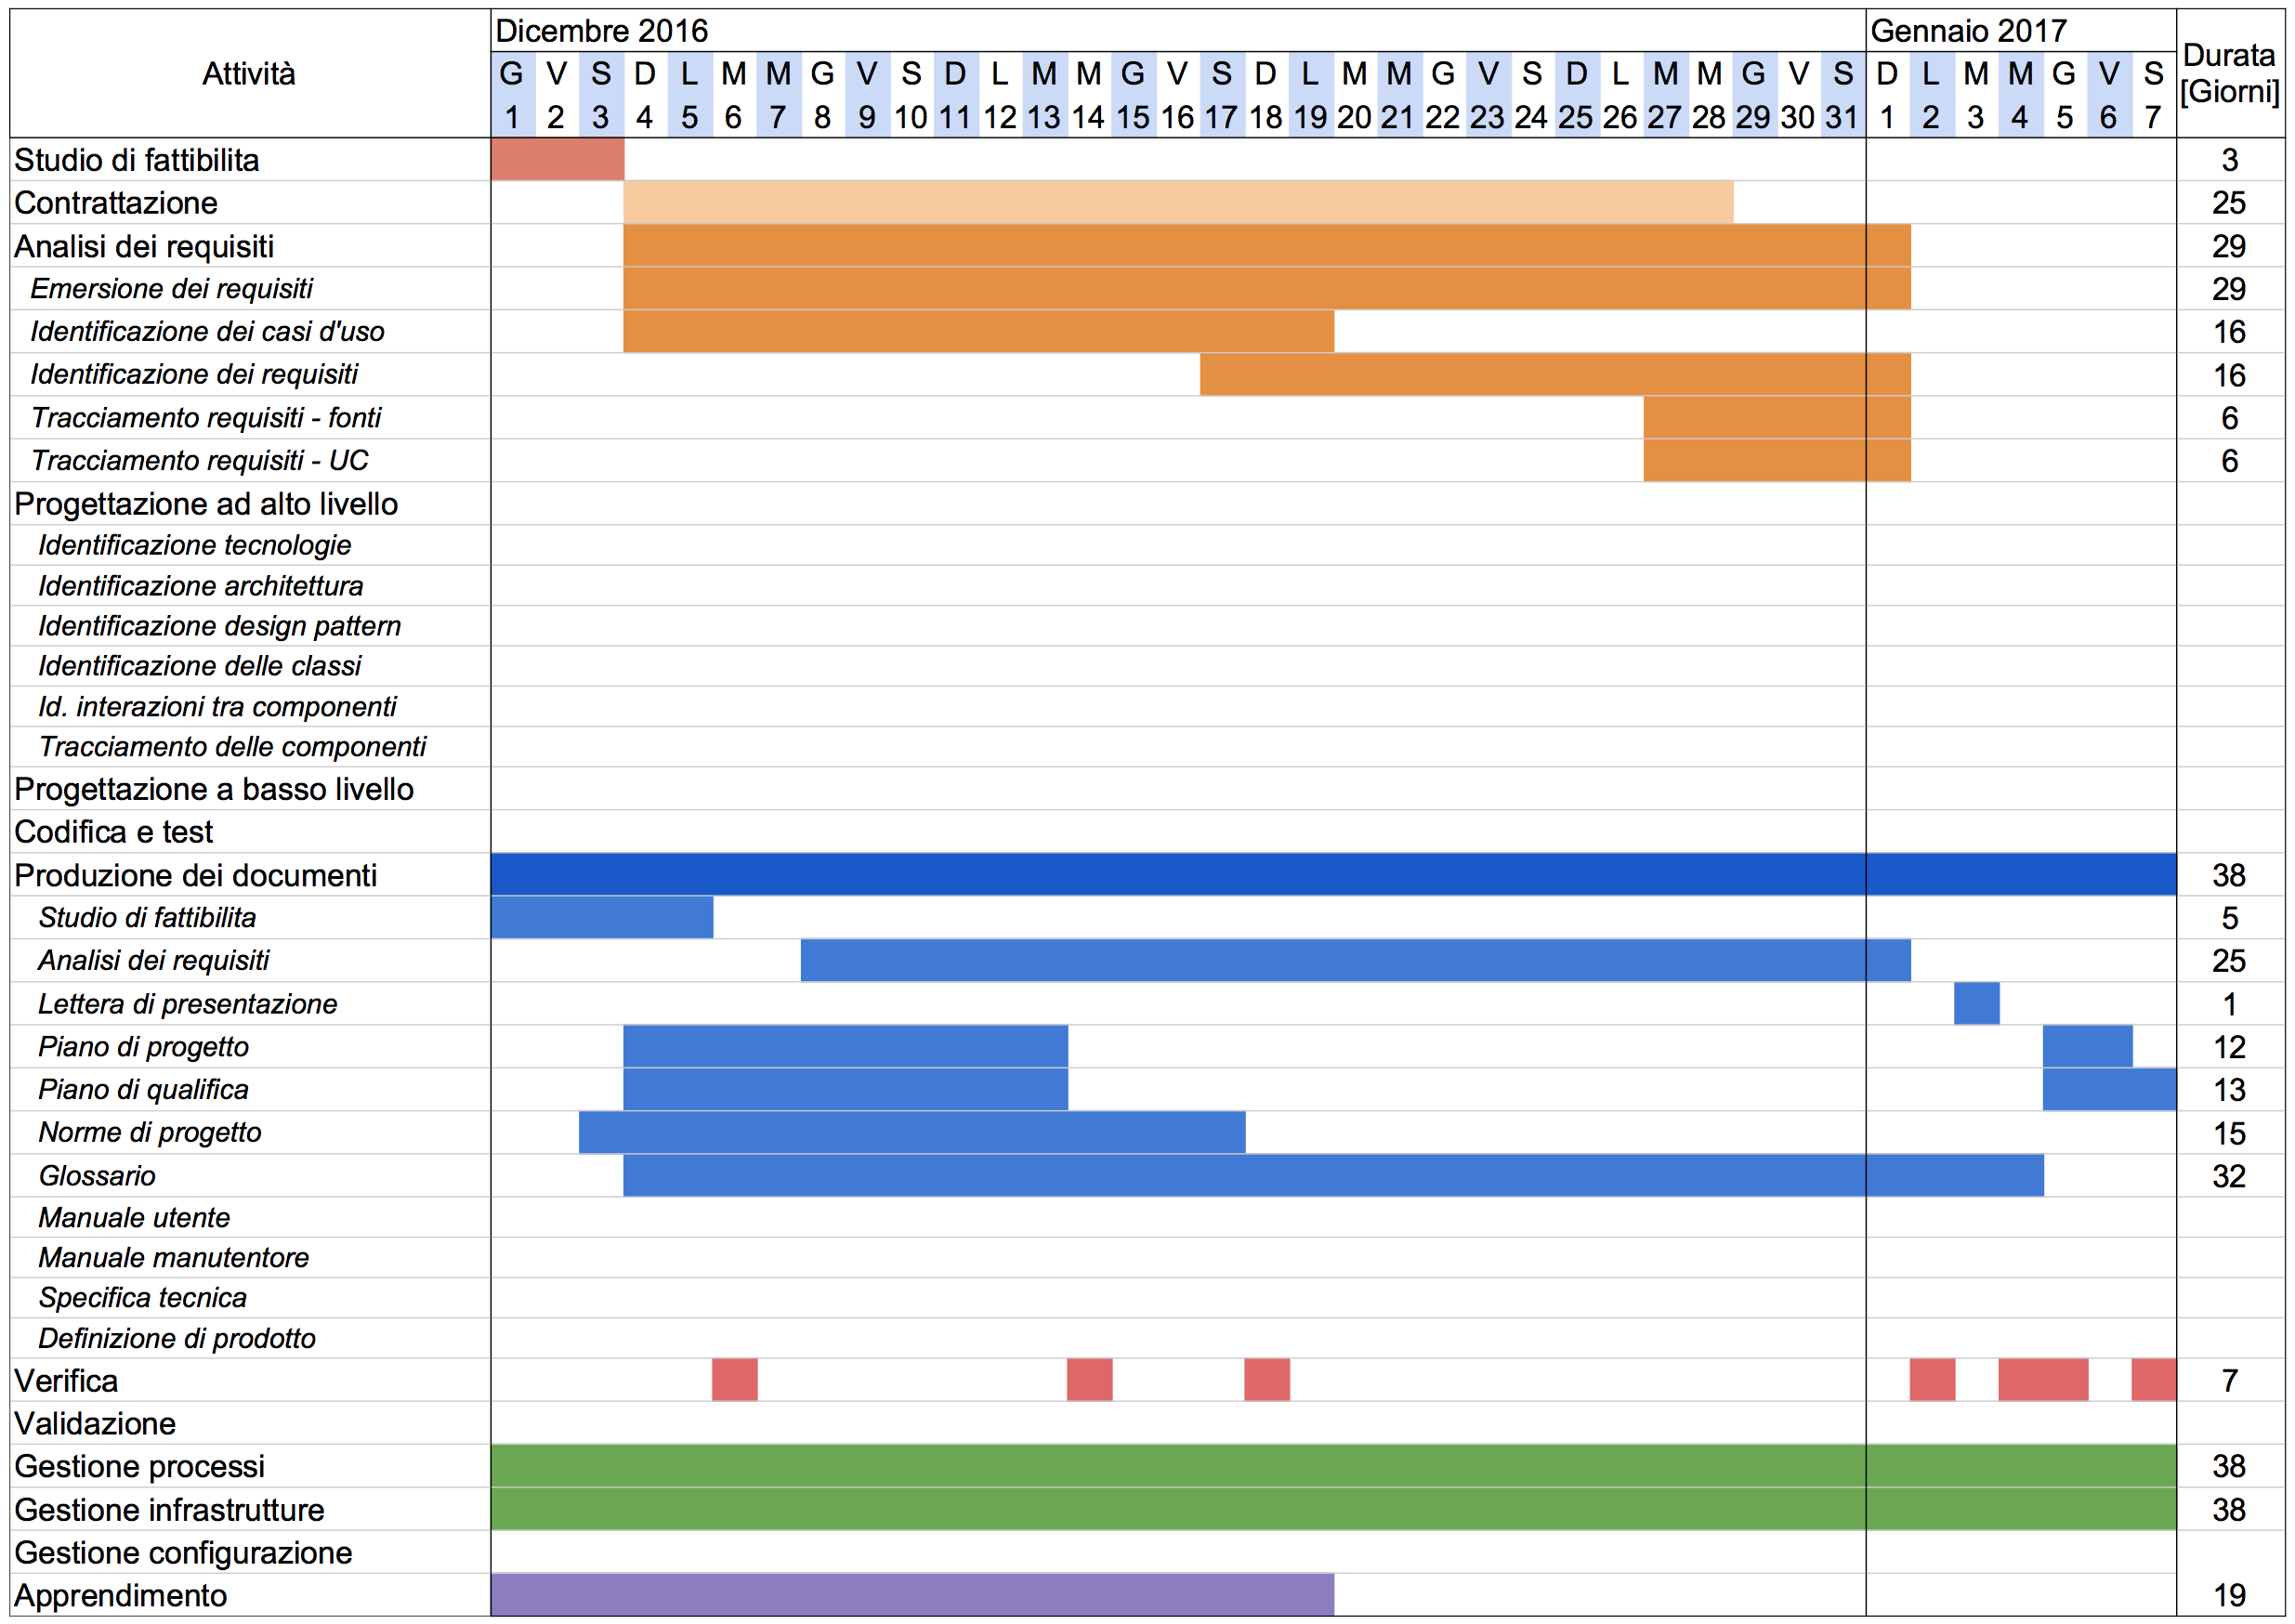
\includegraphics[width=\textwidth]{img/Gantt/g1c.png}
			\caption{Diagramma di Gantt - \glo{Periodo}{Periodo} di analisi}
		\end{figure}
		
	\newpage
	\subsubsection {Progettazione logica}
		\textbf{Periodo}: da \frmdata{12}{01}{2017} a \frmdata{02}{03}{2017} (50 giorni) \\
		Durante questo periodo:
		\begin{itemize}
			\item viene ultimata la raccolta di requisiti;
			\item vengono definiti gli incrementi;
			\item vengono assegnati i requisiti agli incrementi;
			\item viene stabilita l'architettura di massima del sistema.
		\end{itemize}
		Nel corso della progettazione logica verranno quindi individuati gli incrementi, che saranno riportati nel diagramma di Gantt del terzo periodo a partire dalla versione 2.0.0 del \pdp.
		\paragraph{Incrementi individuati}
		Durante il secondo periodo sono stati individuati i seguenti incrementi:
		\begin{itemize}
			\item incremento 1 - mappa;
			\item incremento 2 - \glo{Asset}{asset};
			\item incremento 3 - \glo{Nodo}{nodi};
			\item incremento 4 - \glo{Arco}{archi};
			\item incremento 5 - scenari;
			\item incremento 6 - analisi;
			\item incremento 7 - tutorial;
			\item incremento 8 - assistente vocale.
		\end{itemize}
		\paragraph{Assegnazione dei requisiti agli incrementi}
		Durante il secondo periodo i requisiti presenti nel documento di \adr sono stati assegnati agli incrementi elencati nel paragrafo precedente.
			\begin{table}[H]
				\centering
				\begin{tabular}{ll}
					\toprule
					\textbf{Requisiti}                           & \textbf{Incrementi}              \\
					\midrule
					ROF1 & 2 - asset \\
					ROF2 & 2 - asset \\
					ROF3 & 2 - asset \\
					ROF4 & 2 - asset \\
					ROF5 & 2 - asset \\
					\midrule
					ROF6 & 3 - nodi \\
					ROF7 & 3 - nodi \\
					ROF8 & 3 - nodi \\
					ROF9 & 3 - nodi \\
					ROF10 & 3 - nodi \\
					\midrule
					ROF11 & 4 - archi \\
					ROF12 & 4 - archi \\
					ROF13 & 4 - archi \\
					ROF14 & 4 - archi \\
					ROF15 & 4 - archi \\
					\midrule
					RFF16 & 5 - scenari \\
					RFF17 & 5 - scenari \\
					RFF18 & 5 - scenari \\
					RFF19 & 5 - scenari \\
					RFF20 & 5 - scenari \\
					\midrule
					RFF21 & 6 - analisi \\
					RFF22 & 6 - analisi \\
					RFF23 & 6 - analisi \\
					\midrule
					ROF24 & 1 - mappa \\
					\midrule
					RFF25 & 7 - tutorial \\
					\midrule
					RFF6  & 8 - assistente vocale \\
					\bottomrule
				\end{tabular}
				\caption{Assegnazione dei requisiti agli incrementi}
			\end{table}
		I requisiti non presenti in questa tabella sono da considerarsi implicitamente assegnati ad ogni incremento.
		\paragraph{Processi e attività coinvolte}
			\begin{table}[H]
				\centering
				\begin{tabular}{ll}
					\toprule
					\textbf{Processo}                           & \textbf{Attività}              \\
					\midrule
					\multirow{2}{*}{\textbf{Sviluppo}}          & Analisi dei requisiti          \\
					& Progettazione ad alto livello  \\
					\midrule
					\textbf{Documentazione}            & Produzione dei documenti       \\
					\midrule
					\textbf{Verifica}                  & Verifica                       \\
					\midrule
					\textbf{Gestione processi} 					& Gestione processi              \\
					\midrule
					\textbf{Gestione infrastrutture}				& Gestione infrastrutture        \\
					\midrule
					\textbf{Gestione della configurazione}				& Gestione della configurazione        \\
					\midrule
					\textbf{Apprendimento} 						& Apprendimento                 \\
					\bottomrule
				\end{tabular}
				\caption{Processi e relative attività}
				\label{Pl-ProcessiAttività}
			\end{table}
		\paragraph{Diagramma di Gantt}
		\begin{figure}[H]
			\centering
			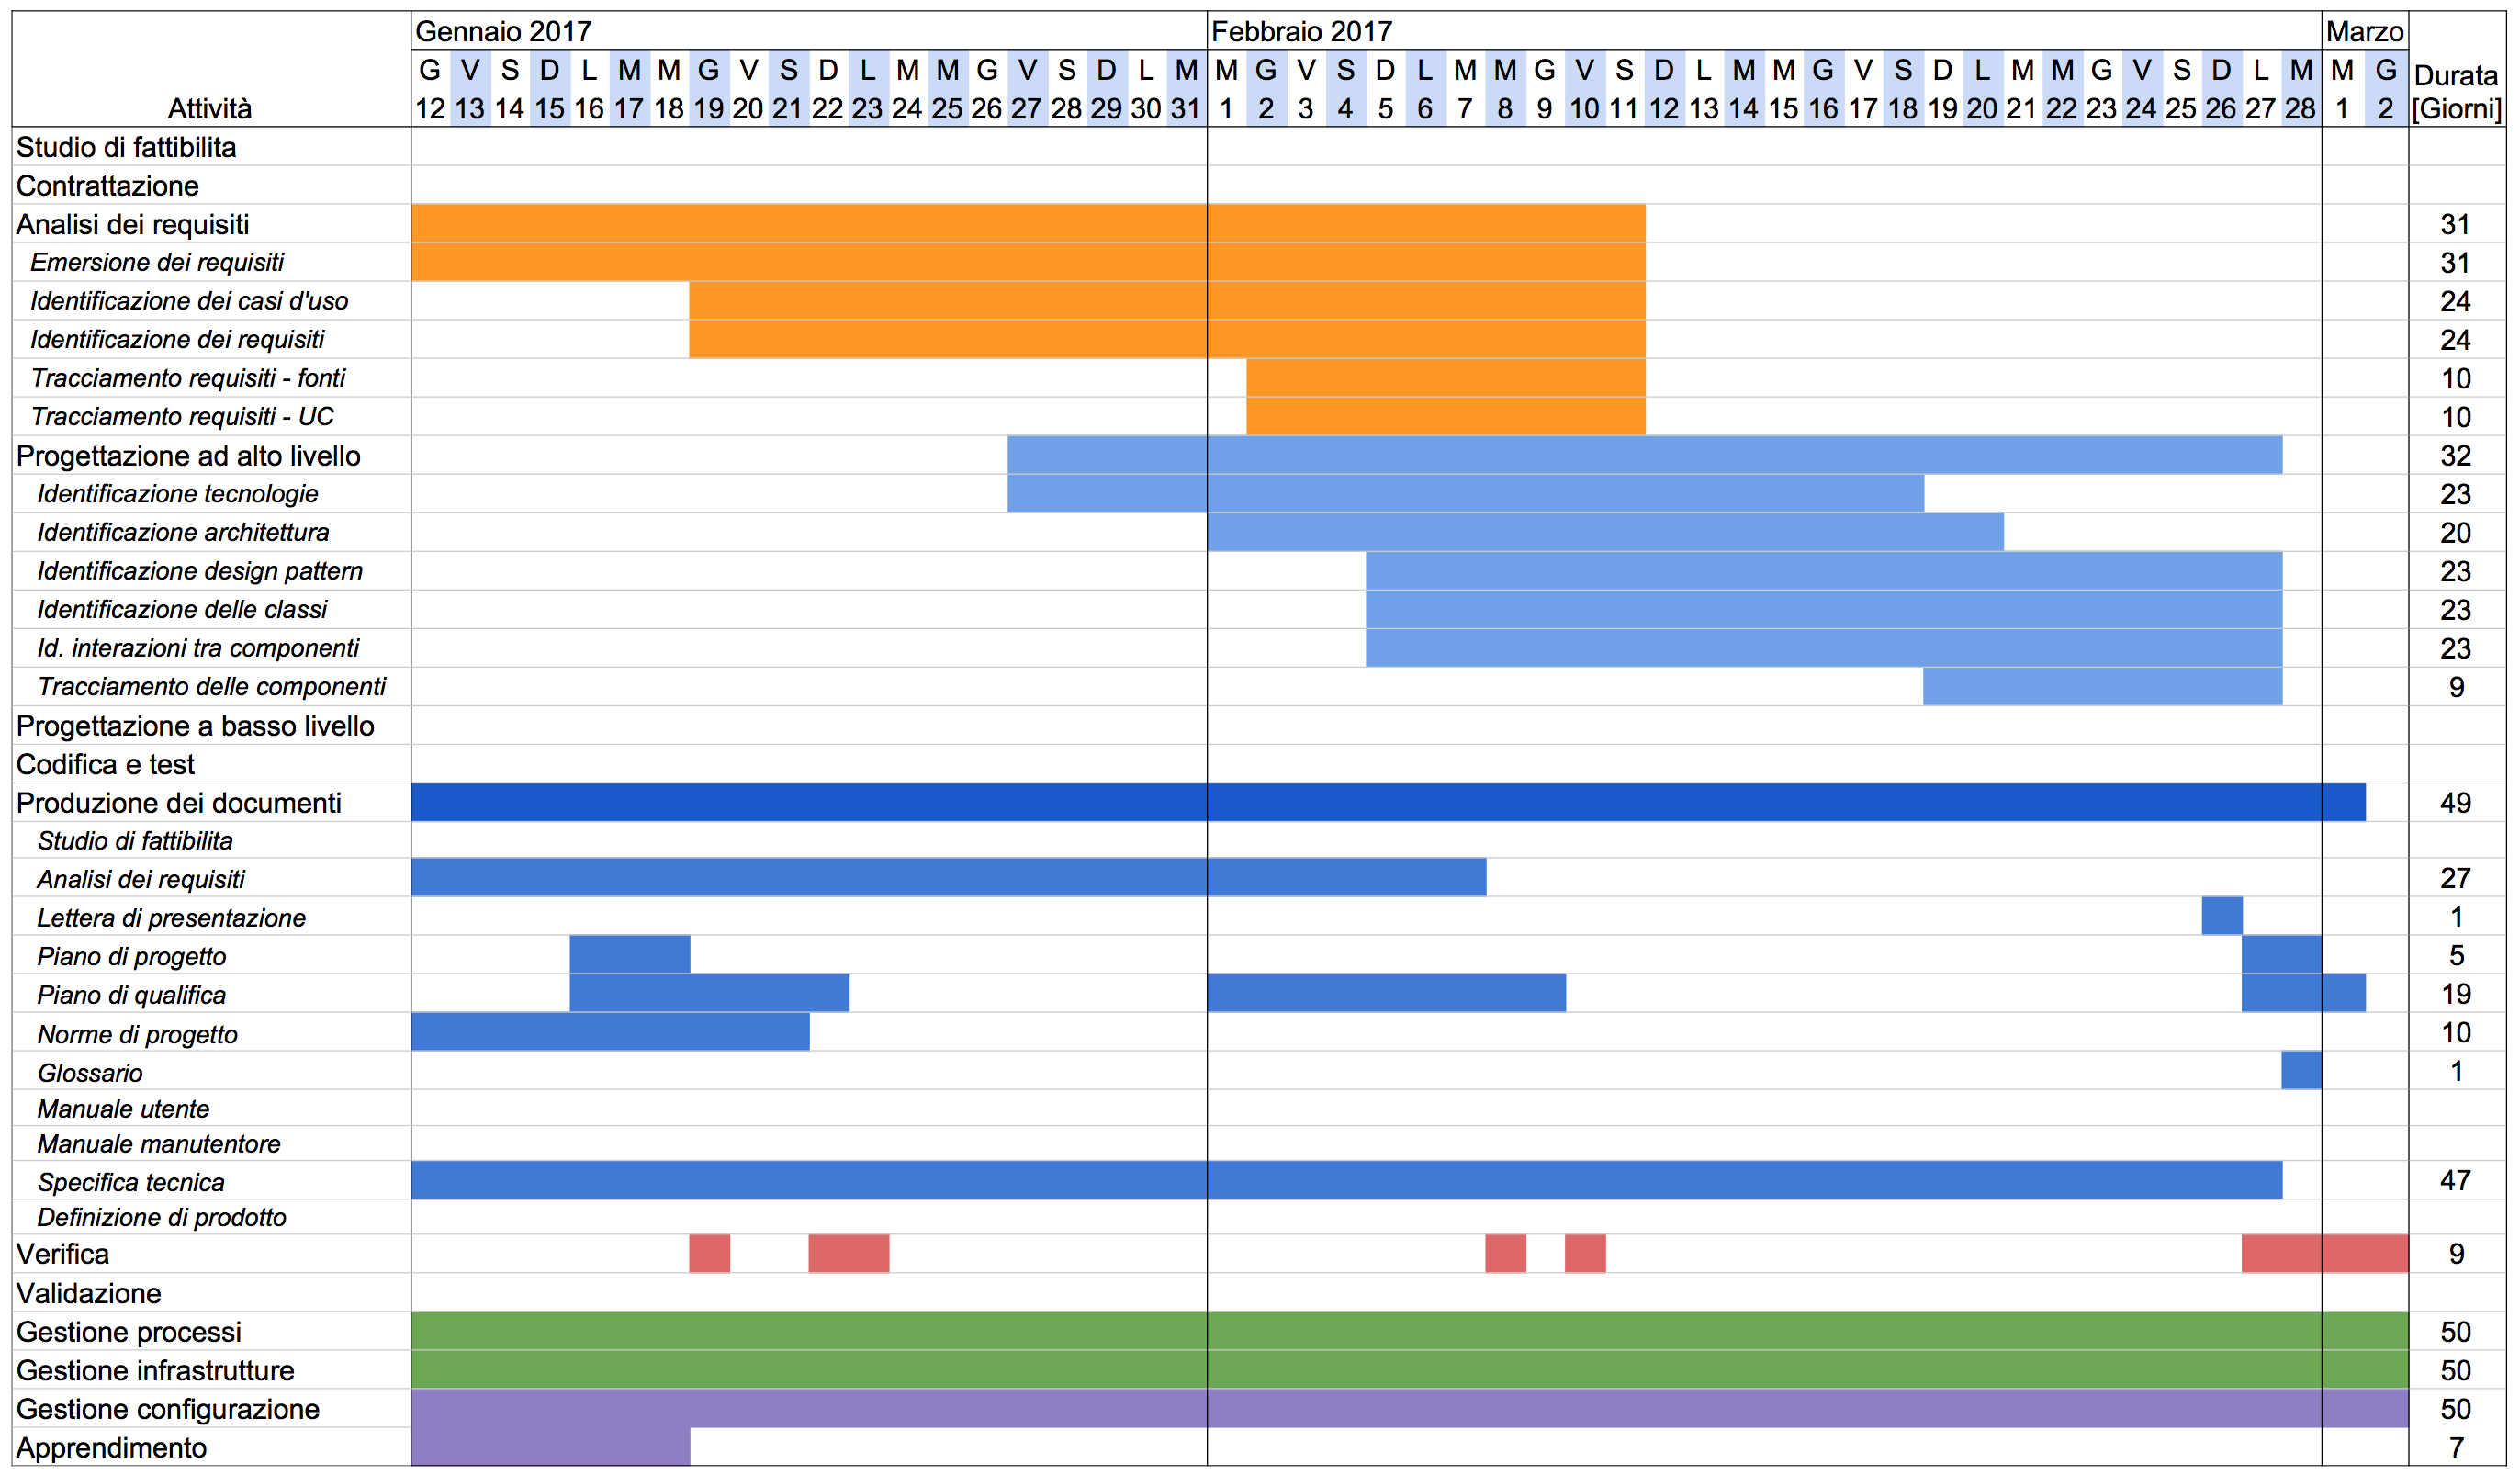
\includegraphics[width=\textwidth]{img/Gantt/g2c.png}
			\caption{Diagramma di Gantt - Periodo di progettazione logica}
		\end{figure}
	
	\newpage
	\subsubsection {Progettazione di dettaglio, codifica e validazione}
		\textbf{Periodo}: da \frmdata{07}{03}{2017} a \frmdata{07}{04}{2017} (31 giorni)\\
		Questo periodo consiste in un ciclo in cui ogni iterazione è data da progettazione, codifica, testing, integrazione del singolo incremento e dalla validazione dell'intero prodotto creato fino a quel momento.
		\\Una volta terminati tutti gli incrementi, il ciclo terminerà.
		\\Le linee verticali presenti nel diagramma indicano i rilasci del sistema validato alla fine dei vari incrementi.
		\paragraph{Processi e attività coinvolte}
			\begin{table}[H]
				\centering
				\begin{tabular}{ll}
					\toprule
					\textbf{Processo}                           & \textbf{Attività}              \\
					\midrule
					\multirow{2}{*}{\textbf{Sviluppo}}          & Progettazione ad basso livello \\
					& Codifica e test \\
					\midrule
					\textbf{Documentazione}            & Produzione dei documenti       \\
					\midrule
					\textbf{Verifica}                  & Verifica                       \\
					\midrule
					\textbf{Validazione}               & Validazione                    \\
					\midrule
					\textbf{Gestione processi} 					& Gestione processi              \\
					\midrule
					\textbf{Gestione infrastrutture}				& Gestione infrastrutture        \\
					\midrule
					\textbf{Gestione della configurazione}				& Gestione della configurazione        \\
					\midrule
					\textbf{Apprendimento} 						& Apprendimento                 \\
					\bottomrule
				\end{tabular}
				\caption{Processi e relative attività}
				\label{Pdrob-ProcessiAttività}
			\end{table}
		\paragraph{Diagramma di Gantt}
		\begin{figure}[H]
			\centering
			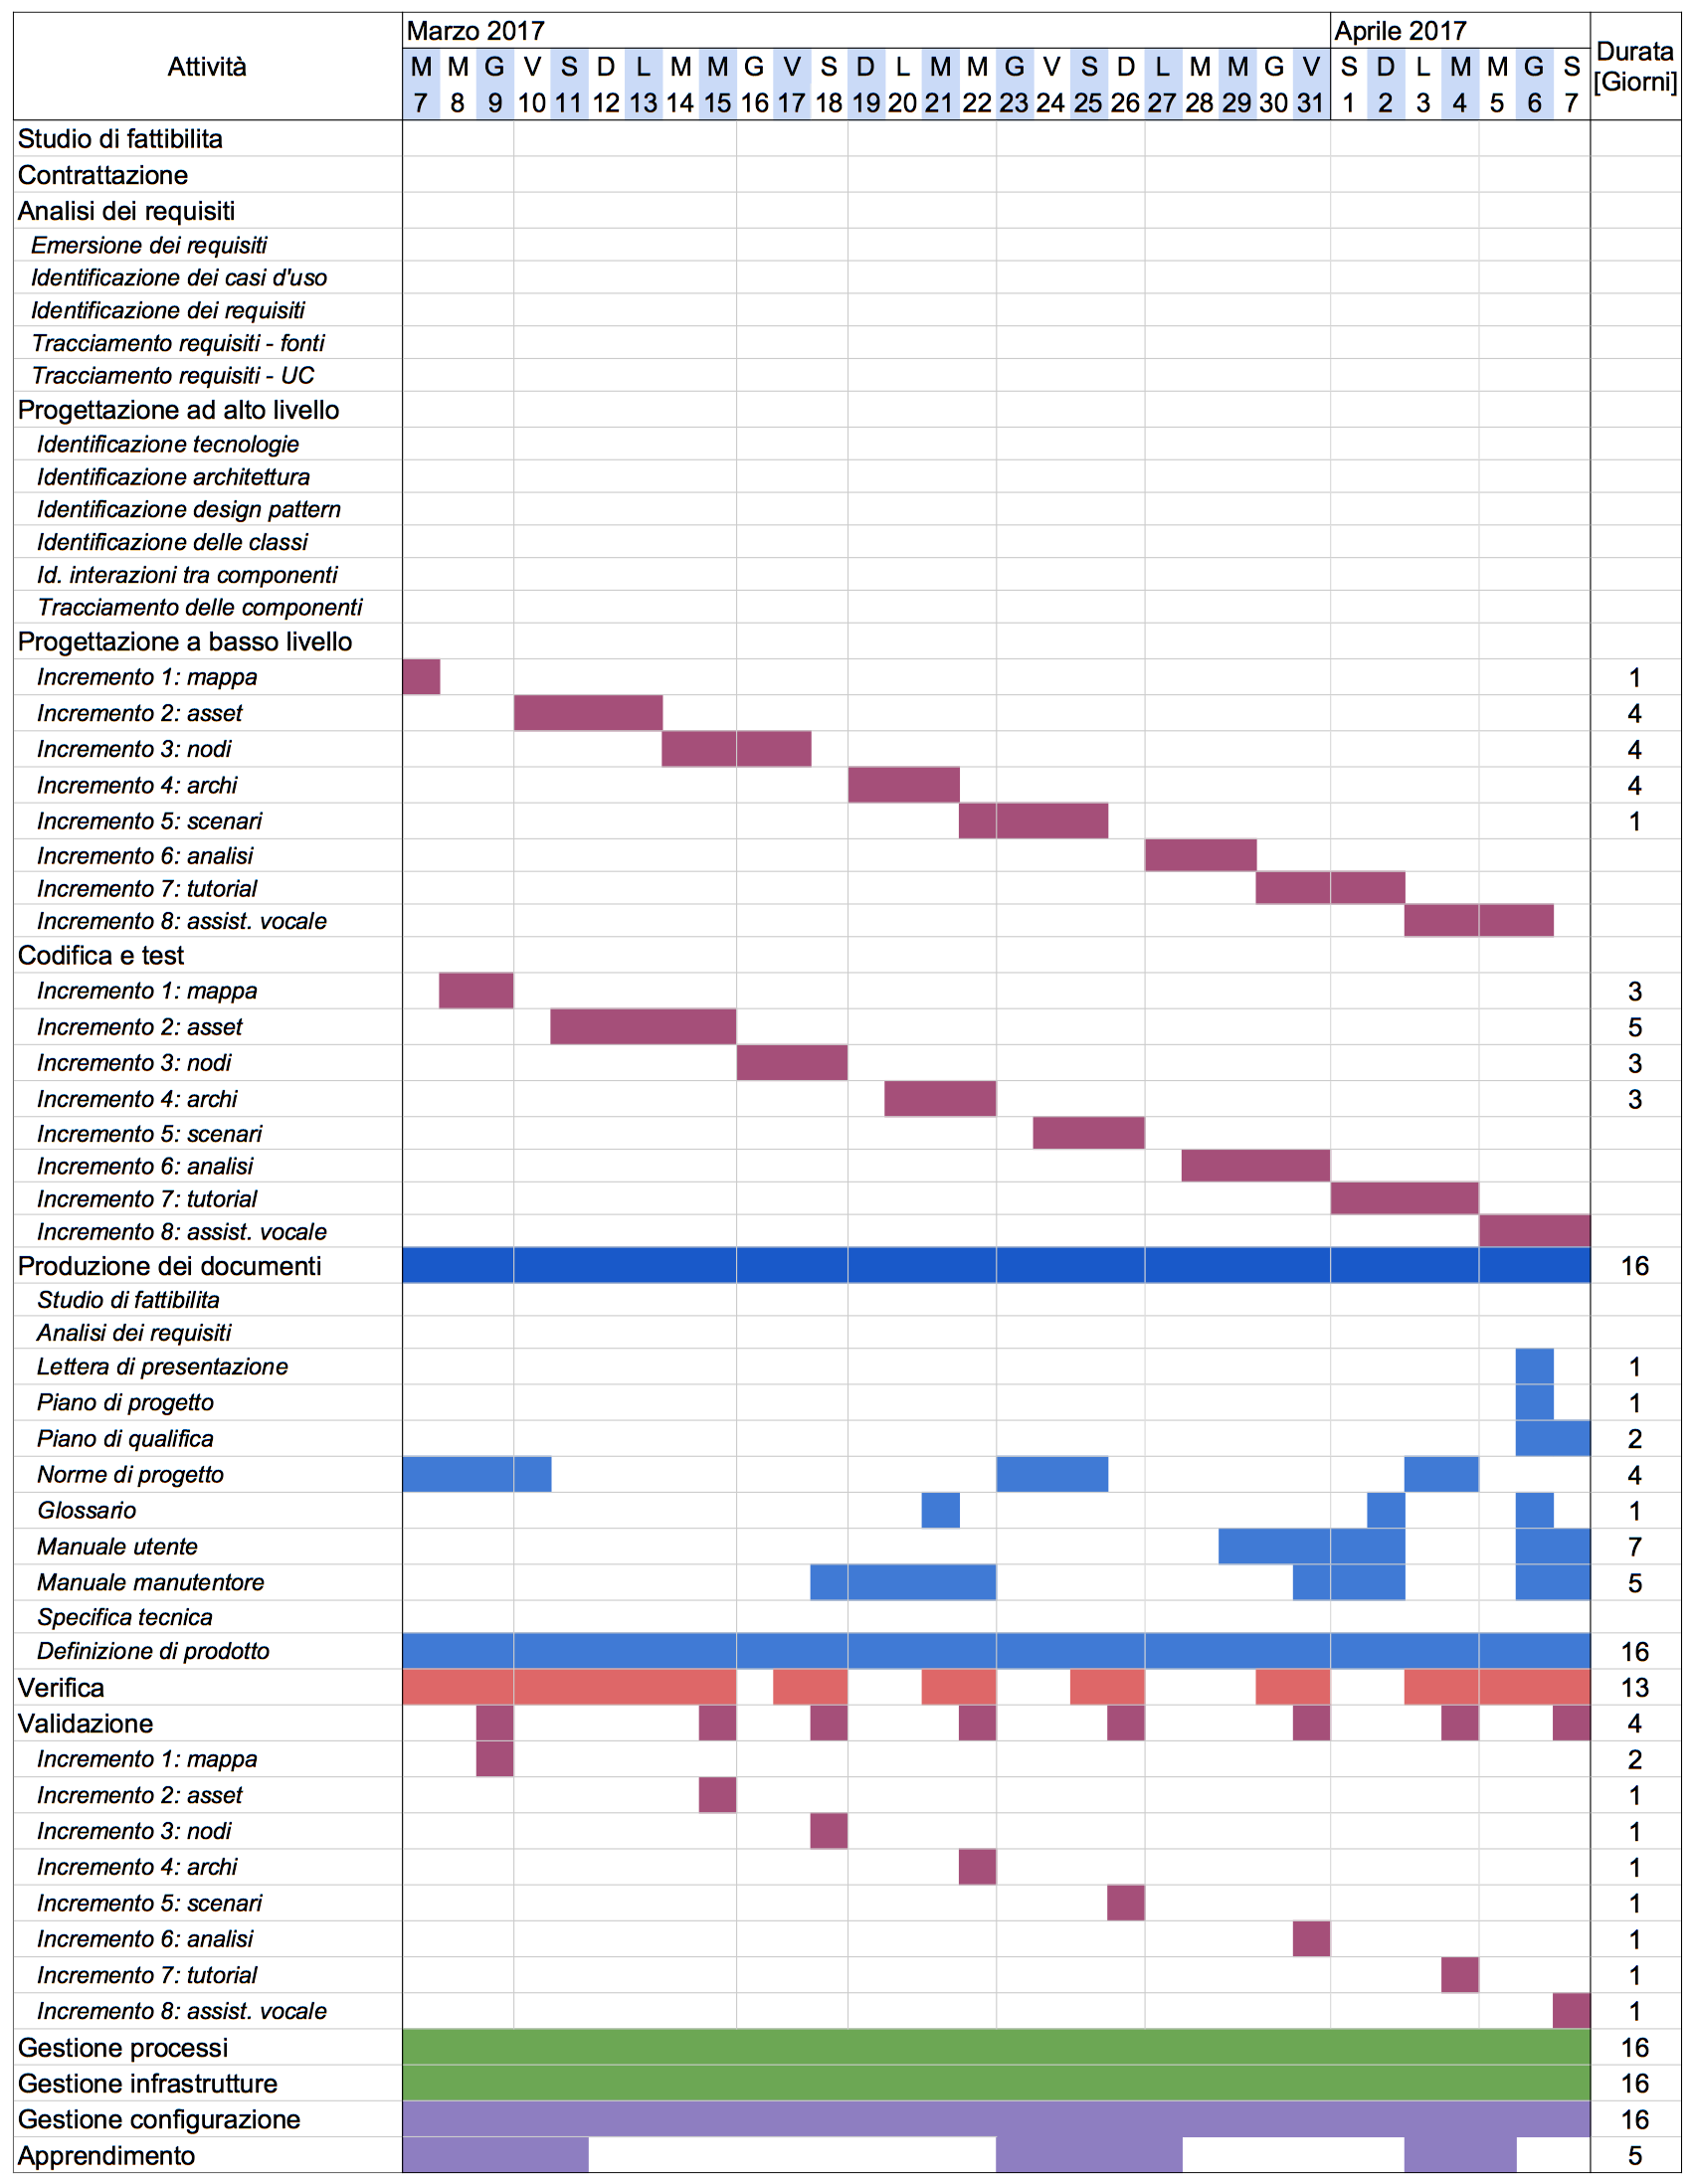
\includegraphics[width=\textwidth]{img/Gantt/g3c.png}
			\caption{Diagramma di Gantt - Periodo di Progettazione di dettaglio Codifica Validazione}
		\end{figure}
		
	\newpage
	\subsubsection {Validazione}
		\textbf{Periodo}: da \frmdata{12}{04}{2017} a \frmdata{04}{05}{2017} (23 giorni) \\
		Durante questo periodo si effettueranno i test di accettazione e il collaudo del sistema.
		\paragraph{Processi e attività coinvolte}
			\begin{table}[H]
				\centering
				\begin{tabular}{ll}
					\toprule
					\textbf{Processo}                           & \textbf{Attività}              \\
					\midrule
					\textbf{Documentazione}            & Produzione dei documenti       \\
					\midrule
					\textbf{Verifica}                  & Verifica                       \\
					\midrule
					\textbf{Validazione}               & Validazione                    \\
					\midrule
					\textbf{Gestione processi} 					& Gestione processi              \\
					\midrule
					\textbf{Gestione infrastrutture}				& Gestione infrastrutture        \\
					\midrule
					\textbf{Gestione della configurazione}				& Gestione della configurazione        \\
					\bottomrule
				\end{tabular}
				\caption{Processi e relative attività}
				\label{Va-ProcessiAttività}
			\end{table}
		\paragraph{Diagramma di Gantt}
		\begin{figure}[H]
			\centering
			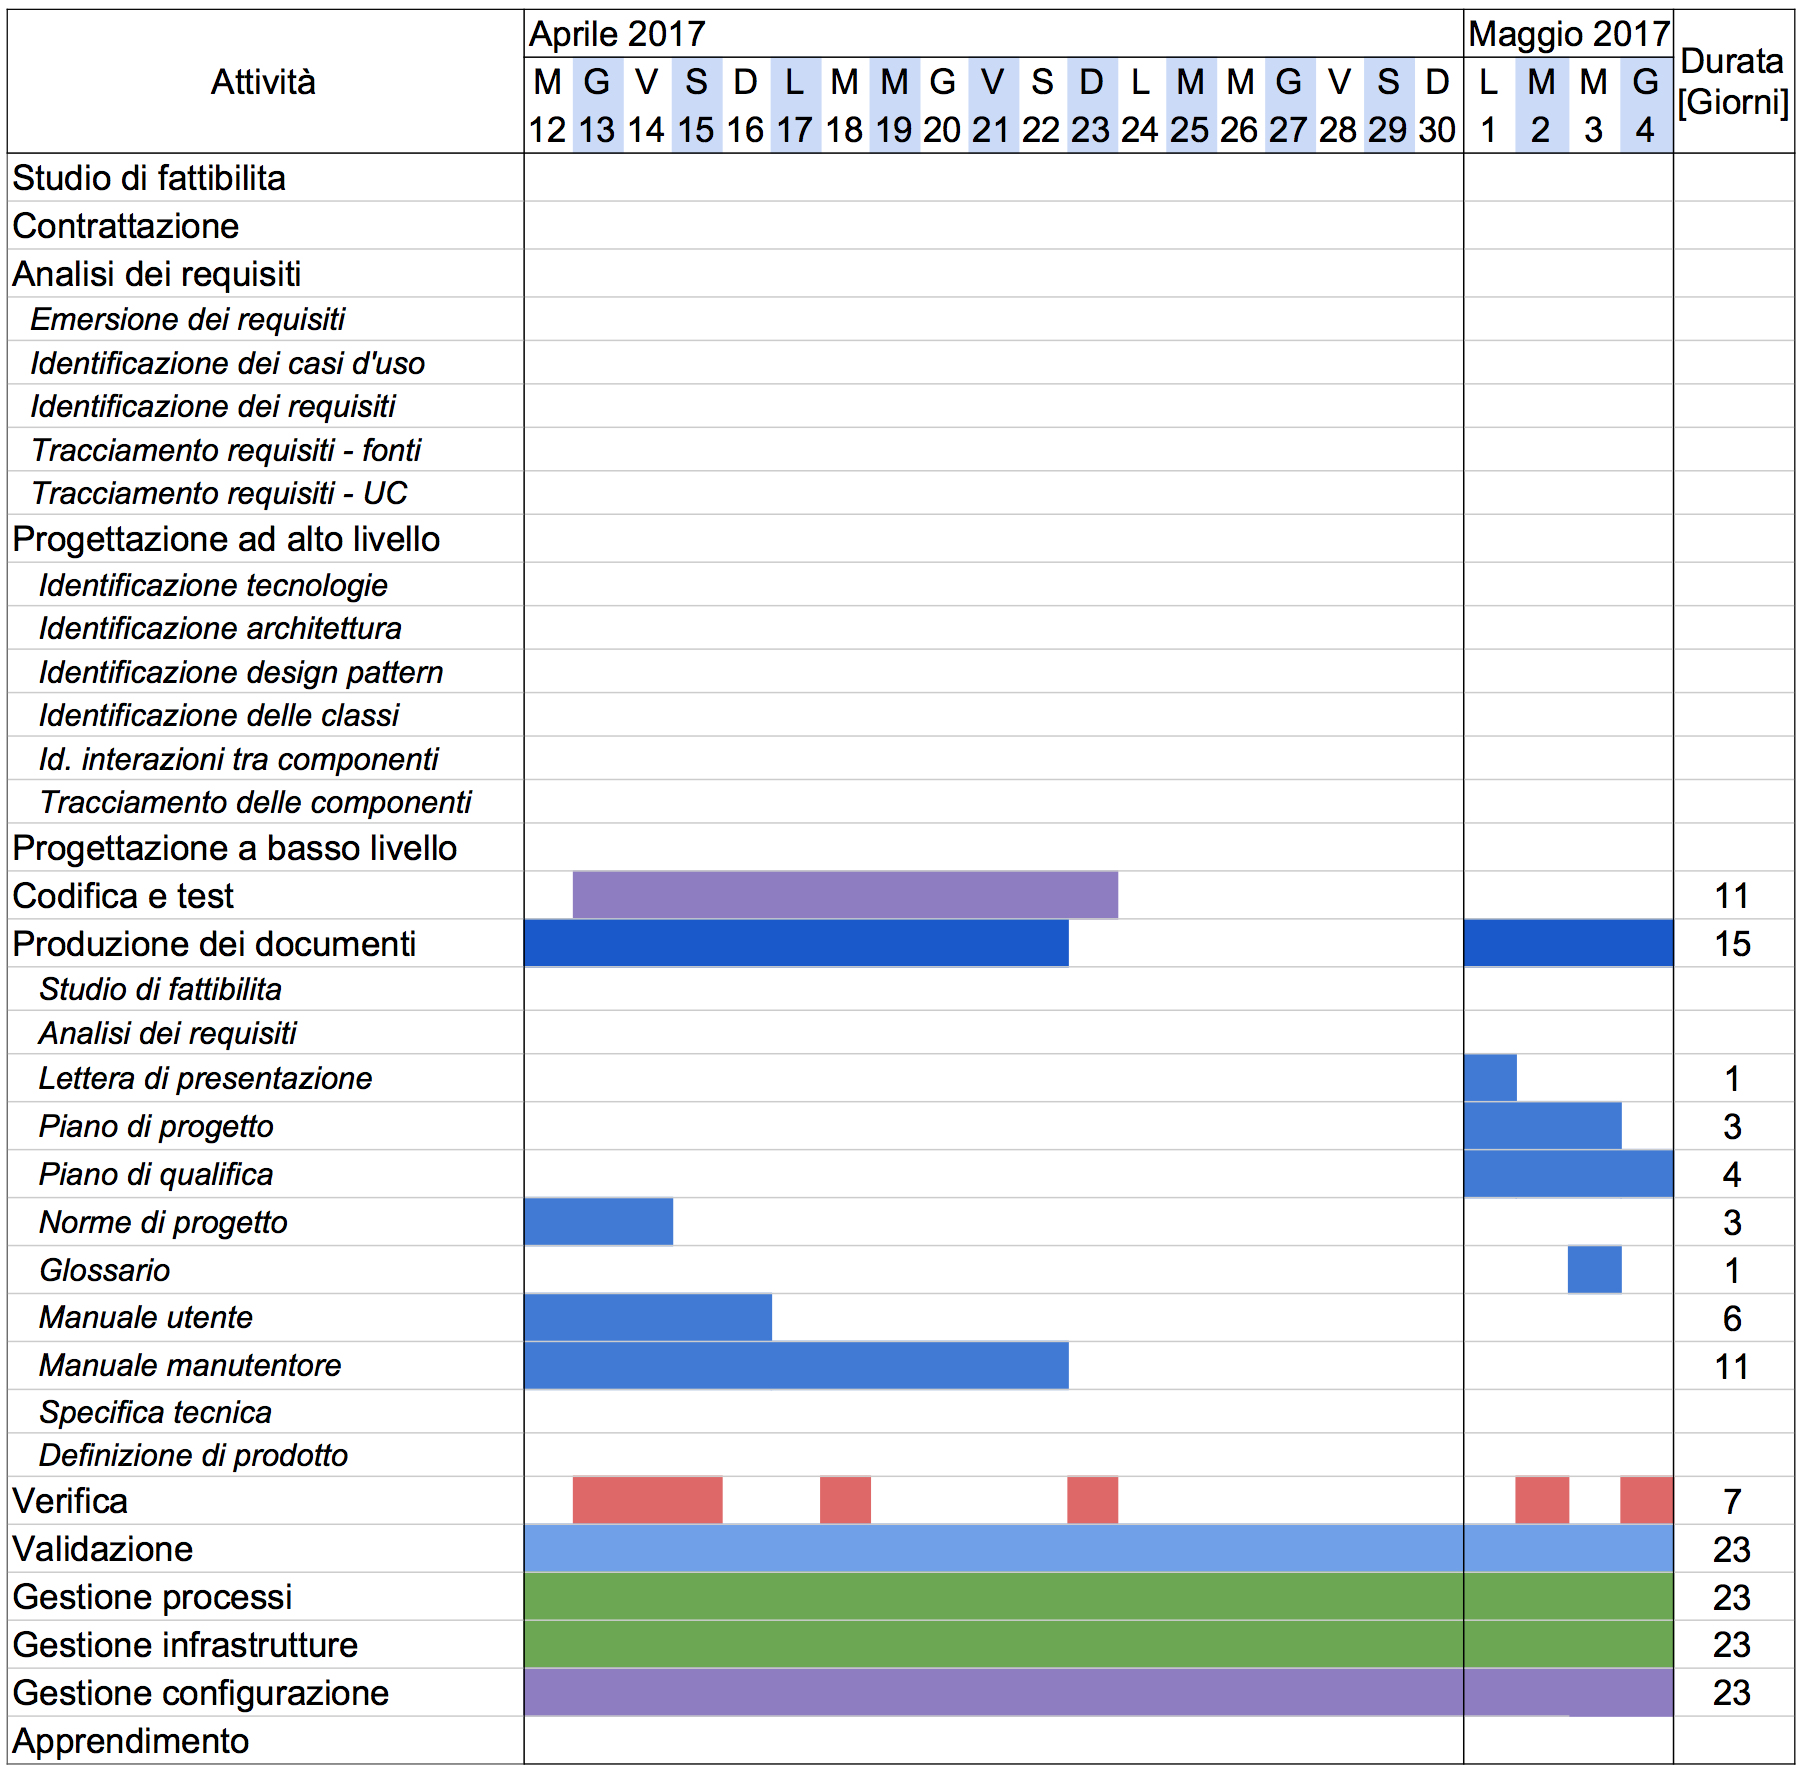
\includegraphics[width=\textwidth]{img/Gantt/g4c.png}
			\caption{Diagramma di Gantt - Periodo di validazione}
		\end{figure}
		
			\newpage
			\subsubsection {Validazione - Pianificazione correttiva}
			\textbf{Periodo}: da \frmdata{12}{04}{2017} a \frmdata{18}{08}{2017} (128 giorni) \\
			In seguito all'esito della Revisione di Qualifica, si sono tenuti alcuni incontri tra i membri del gruppo e sono state prese importanti decisioni riguardo la consegna del progetto (vedi Verbale interno 6). In particolare si è deciso di consegnare il prodotto finale nella revisione di avanzamento del 22 agosto. Durante questo periodo dovranno essere effettuate opportune manovre correttive appositamente scelte per migliorare sul piano tecnico il prodotto consegnato in sede di Revisione di Qualifica, per poi passare a concludere i test di unità, integrazione e sistema mancanti. Infine come da piani precedentemente fissati, il gruppo si occuperà dei test di accettazione e il collaudo del sistema. La correzione di quanto presentato in Revisione di Qualifica ha portato alla reintroduzione del processo di sviluppo in questo periodo ed è da considerarsi una iterazione che figurerà nelle ore non rendicontate.
			\paragraph{Processi e attività coinvolte}
			\begin{table}[H]
				\centering
				\begin{tabular}{ll}
					\toprule
					\textbf{Processo}                           & \textbf{Attività}              \\
					\midrule
					\multirow{2}{*}{\textbf{Sviluppo}}          & Progettazione ad basso livello \\
					& Codifica e test \\
					\midrule
					\textbf{Documentazione}            & Produzione dei documenti       \\
					\midrule
					\textbf{Verifica}                  & Verifica                       \\
					\midrule
					\textbf{Validazione}               & Validazione                    \\
					\midrule
					\textbf{Gestione processi} 					& Gestione processi              \\
					\midrule
					\textbf{Gestione infrastrutture}				& Gestione infrastrutture        \\
					\midrule
					\textbf{Gestione della configurazione}				& Gestione della configurazione        \\
					\midrule
					\textbf{Apprendimento} 						& Apprendimento                 \\
					\bottomrule
				\end{tabular}
				\caption{Processi e relative attività}
				\label{VaCorr-ProcessiAttività}
			\end{table}
			\paragraph{Diagramma di Gantt}
			\begin{figure}[H]
				\centering
				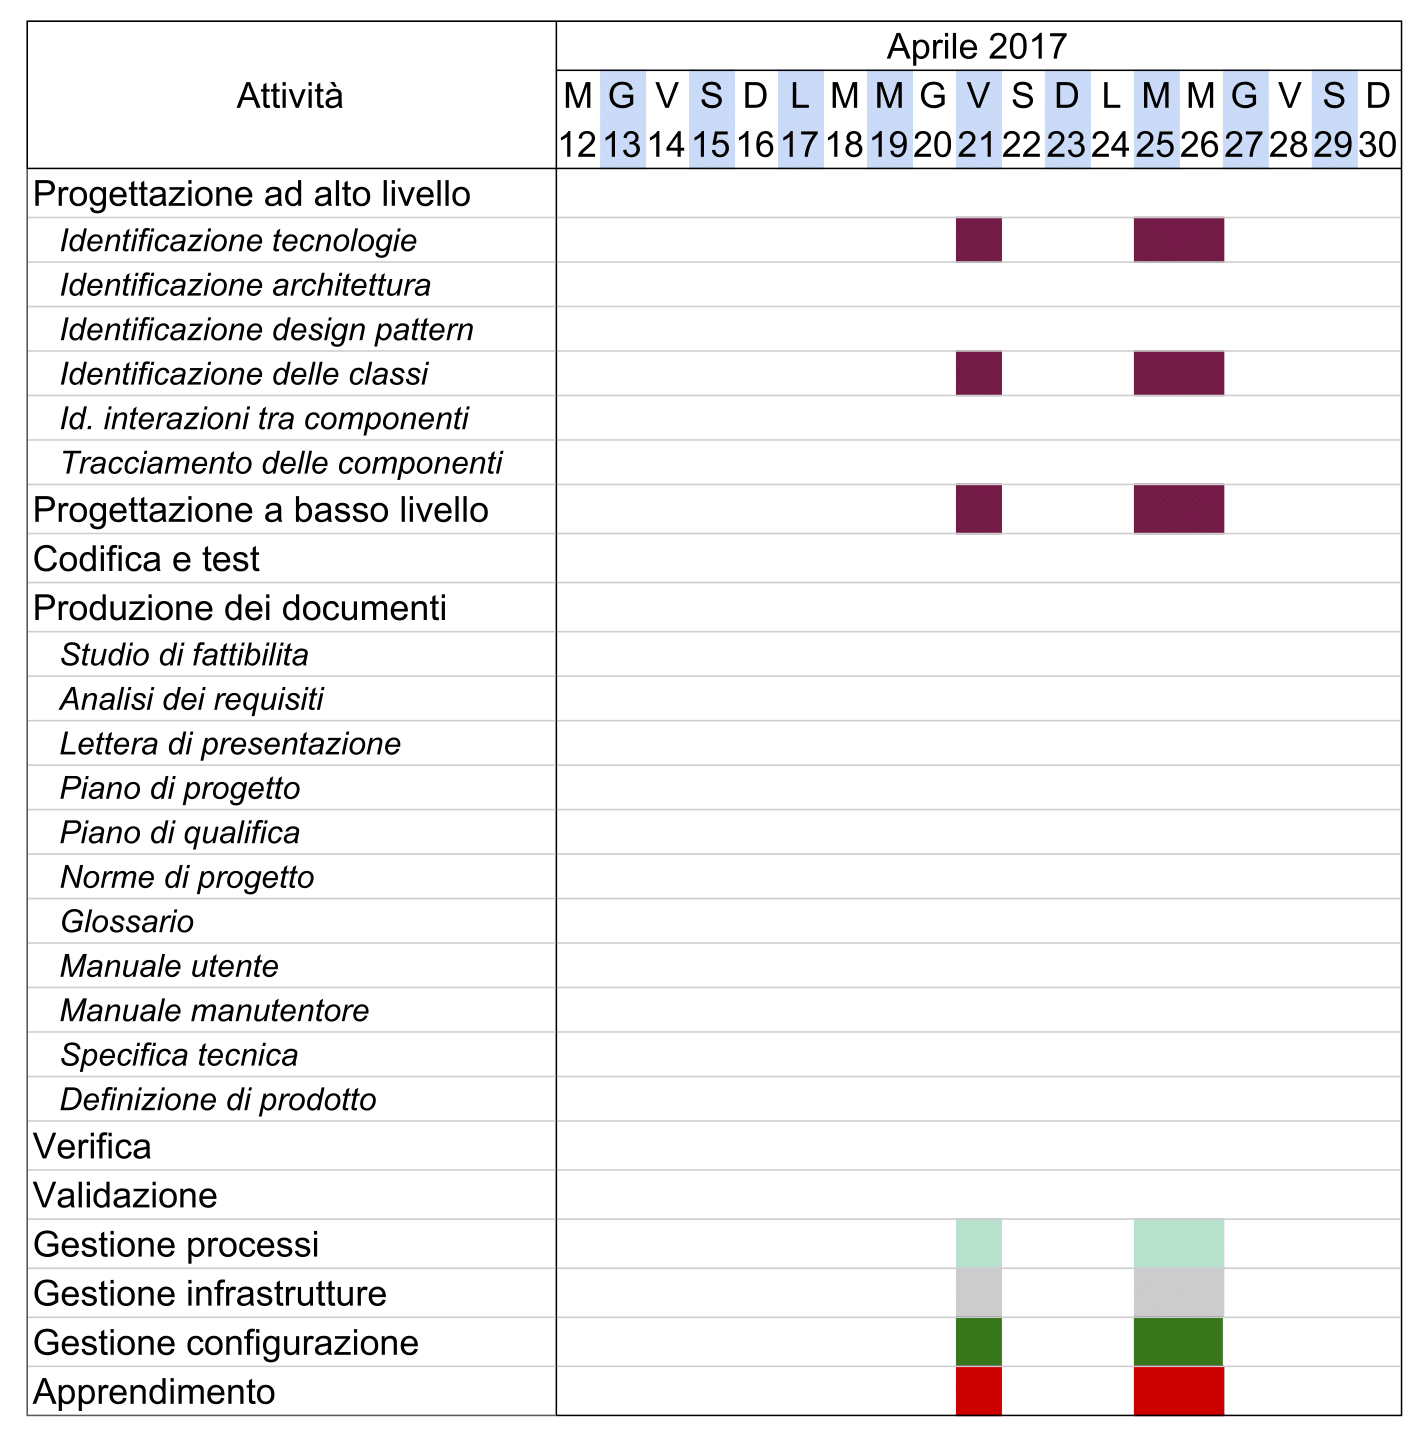
\includegraphics[width=\textwidth]{img/Gantt/FiAprile.png}
				\caption{Diagramma di Gantt - Periodo di Validazione - Pianificazione correttiva Aprile}
			\end{figure}
			\newpage
			\begin{figure}[H]
				\centering
				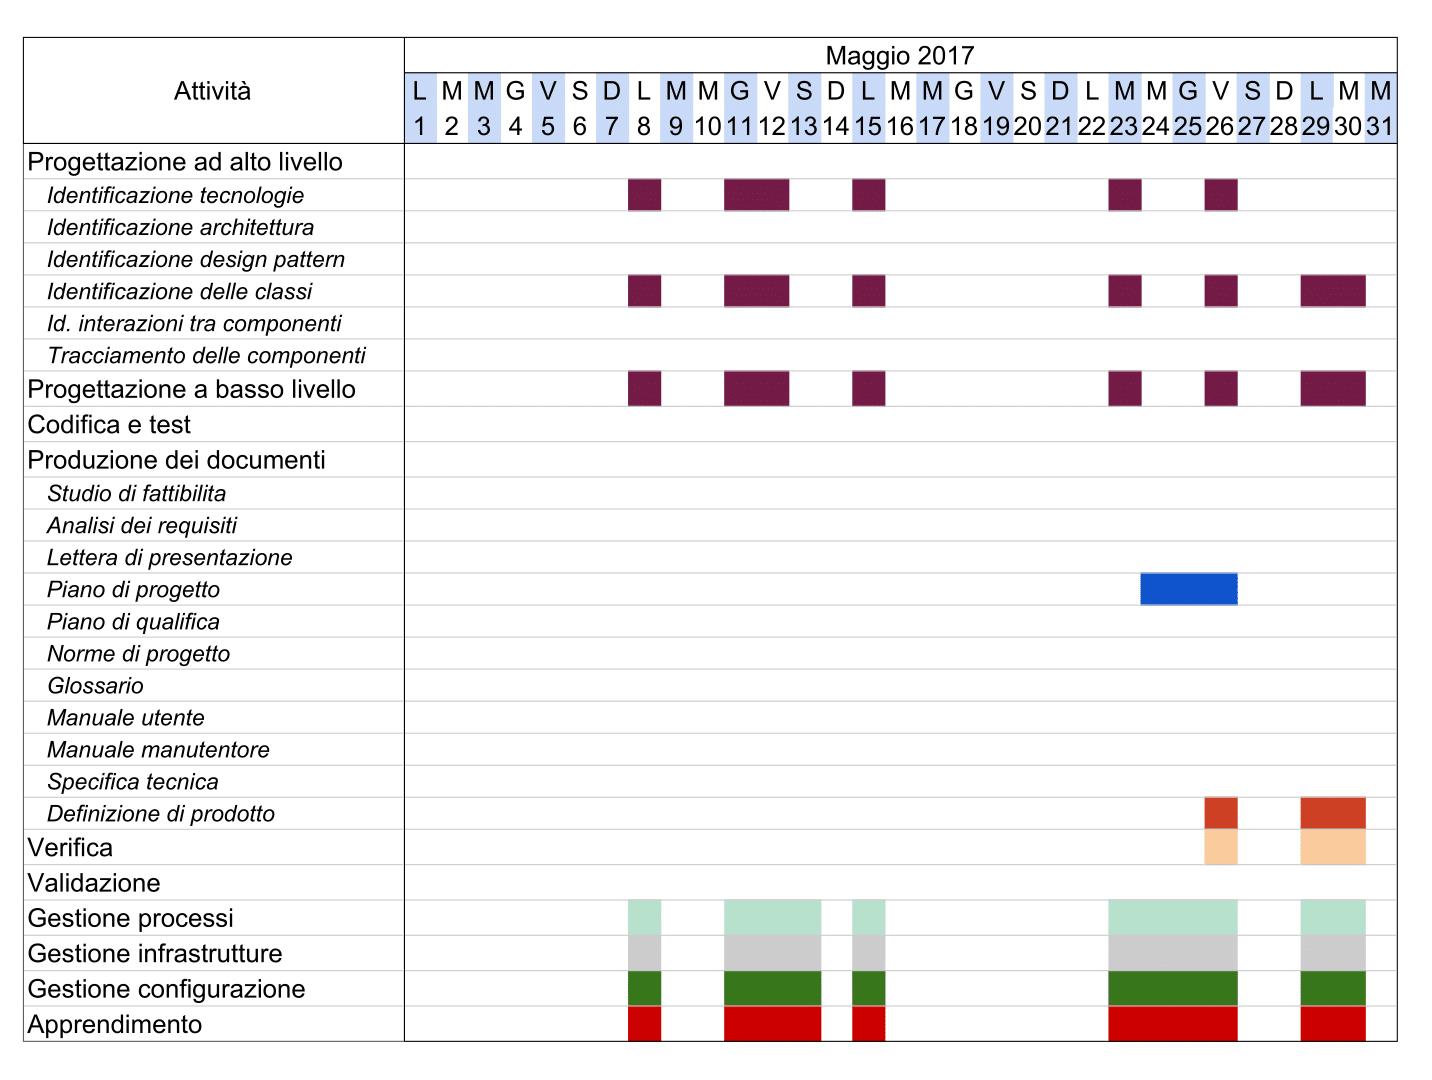
\includegraphics[width=\textwidth]{img/Gantt/FiMaggio.png}
				\caption{Diagramma di Gantt - Periodo di Validazione - Pianificazione correttiva Maggio}
			\end{figure}
			\newpage
			\begin{figure}[H]
				\centering
				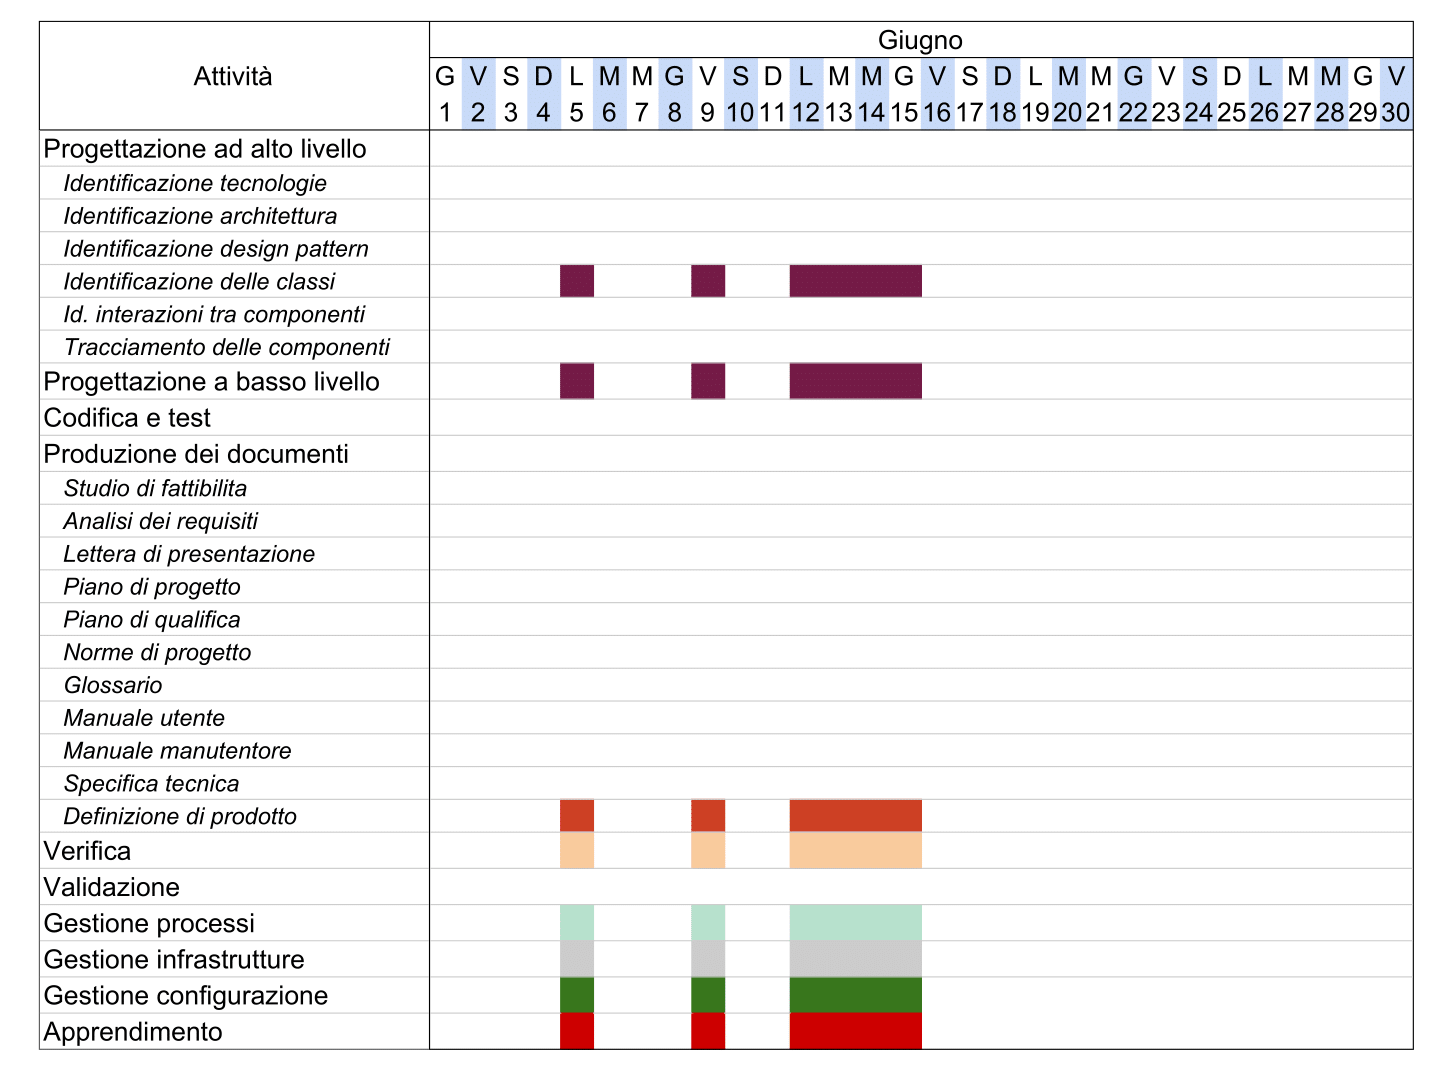
\includegraphics[width=\textwidth]{img/Gantt/FiGiugno.png}
				\caption{Diagramma di Gantt - Periodo di Validazione - Pianificazione correttiva Giugno}
			\end{figure}			\newpage
			\begin{figure}[H]
				\centering
				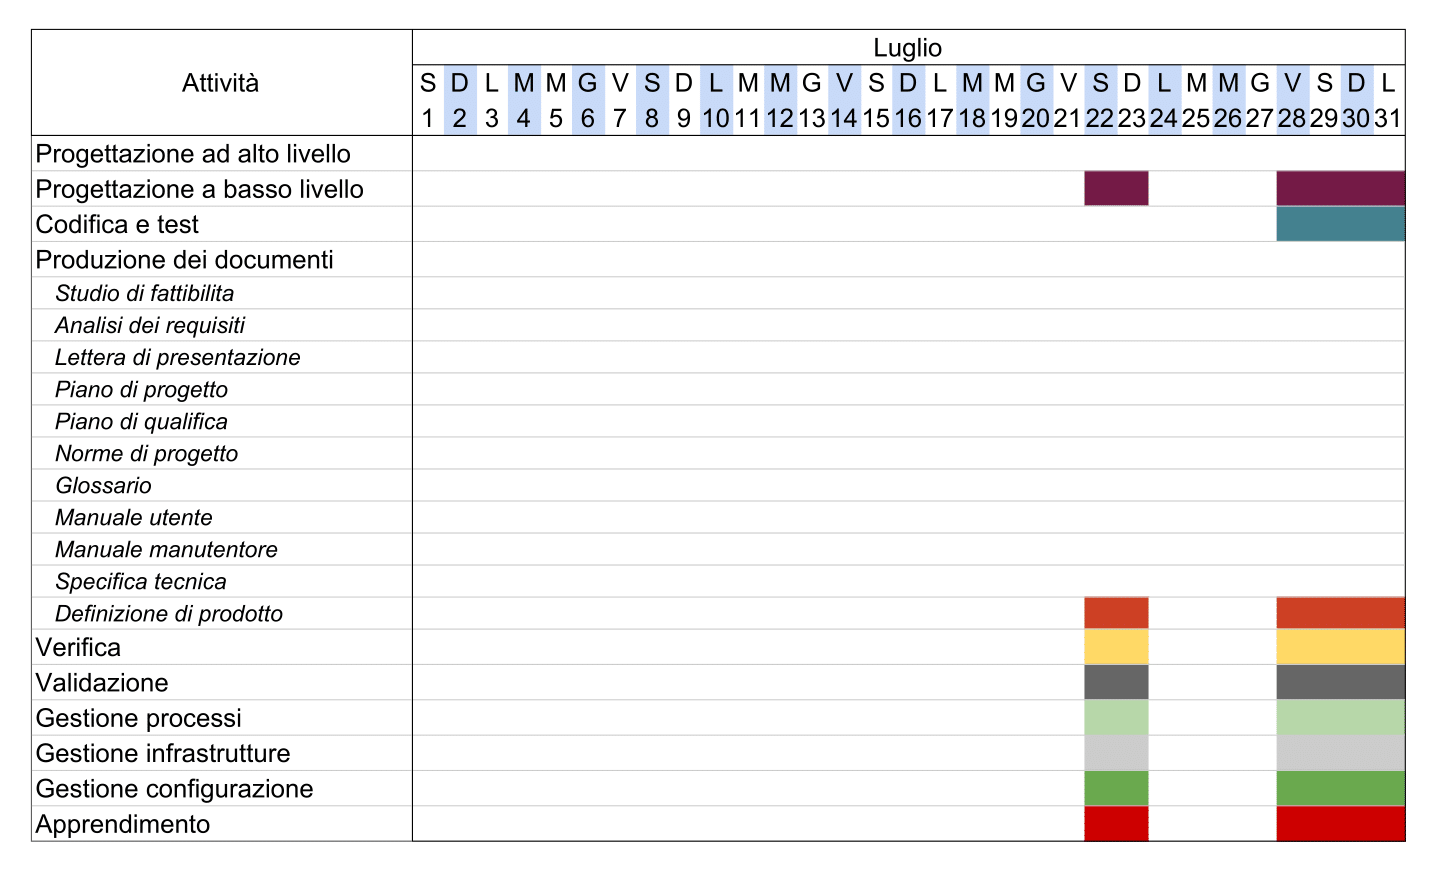
\includegraphics[width=\textwidth]{img/Gantt/FiLuglio.png}
				\caption{Diagramma di Gantt - Periodo di Validazione - Pianificazione correttiva Luglio}
			\end{figure}
			\newpage
			\begin{figure}[H]
				\centering
				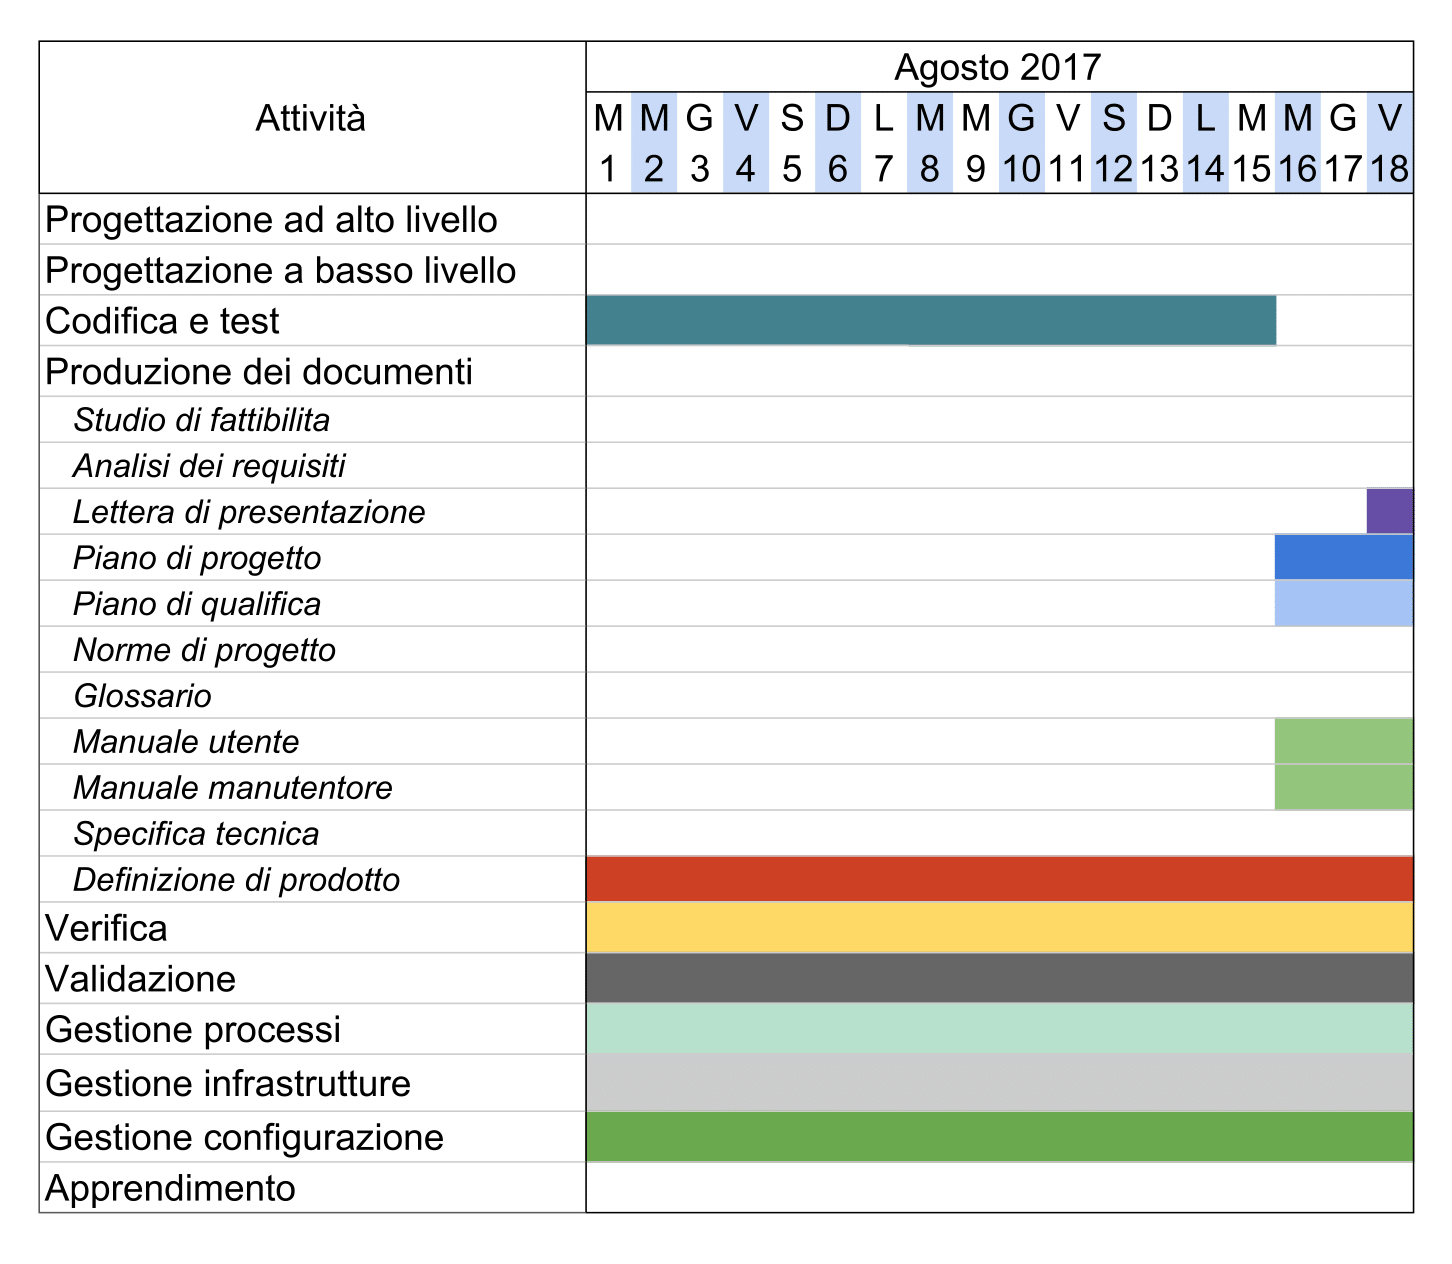
\includegraphics[width=\textwidth]{img/Gantt/FiAgosto.png}
				\caption{Diagramma di Gantt - Periodo di Validazione - Pianificazione correttiva Agosto}
			\end{figure}

	%\section {Preventivo}
\section {Preventivo}
	\subsection {Introduzione}
    In questa sezione viene descritta la suddivisione del lavoro in vari \glo{Periodo}{periodi} e l'assegnazione ai membri del \glo{Gruppo}{gruppo} in base ai ruoli ricoperti. Verrà posta particolare attenzione all'aspetto economico.
    Verranno utilizzate le seguenti abbreviazioni:
   		\begin{itemize}
   		\item{\textbf{Re}}: \responsabilediprogetto;
     	\item{\textbf{Am}}: \amministratore;
     	\item{\textbf{At}}: \analista;
     	\item{\textbf{Pj}}: \progettista;
     	\item{\textbf{Pr}}: \programmatore;
     	\item{\textbf{Ve}}: \verificatore;
     	\item{\textbf{Tot}}: totale.
   		\end{itemize}

\newpage
	\subsection {Dettaglio periodi}
		\subsubsection {Periodo: An - Analisi}
			\paragraph{Preventivo orario}
%-----------------------------------------------------------------
							\begin{table}[H] \begin{center} \begin{tabular}{llllllll}
							\toprule
							\textbf{Nominativo}	&	\textbf{Re}	&	\textbf{Am}	&	\textbf{At}	&	\textbf{Pj}	&	\textbf{Pr}	&	\textbf{Ve}	&	\textbf{Tot}\\
							\midrule
							Brutesco	&	-	&	-	&	12	&	-	&	-	&	12	&	24	 \\
							Damo		&	-	&	9	&	15	&	-	&	-	&	-	&	24	 \\
							De Gaspari	&	-	&	-	&	12	&	-	&	-	&	12	&	24	 \\
							Gottardo	&	14	&	-	&	10	&	-	&	-	&	-	&	24	 \\
							Pasqualini	&	-	&	-	&	12	&	-	&	-	&	12	&	24	 \\
							Petenazzi	&	7	&	-	&	17	&	-	&	-	&	-	&	24	 \\
							Prete		&	-	&	10	&	14	&	-	&	-	&	-	&	24	 \\
							\midrule
							Tot. in ore	&	21	&	19	&	92	&	0	&	0	&	36	&	168	 \\

							\bottomrule
							\end{tabular} \end{center} \caption{Prospetto orario - \glo{Periodo}{Periodo}:
							An
							}\label{tab:h_An} \end{table}

								\begin{figure}[H]  \centering  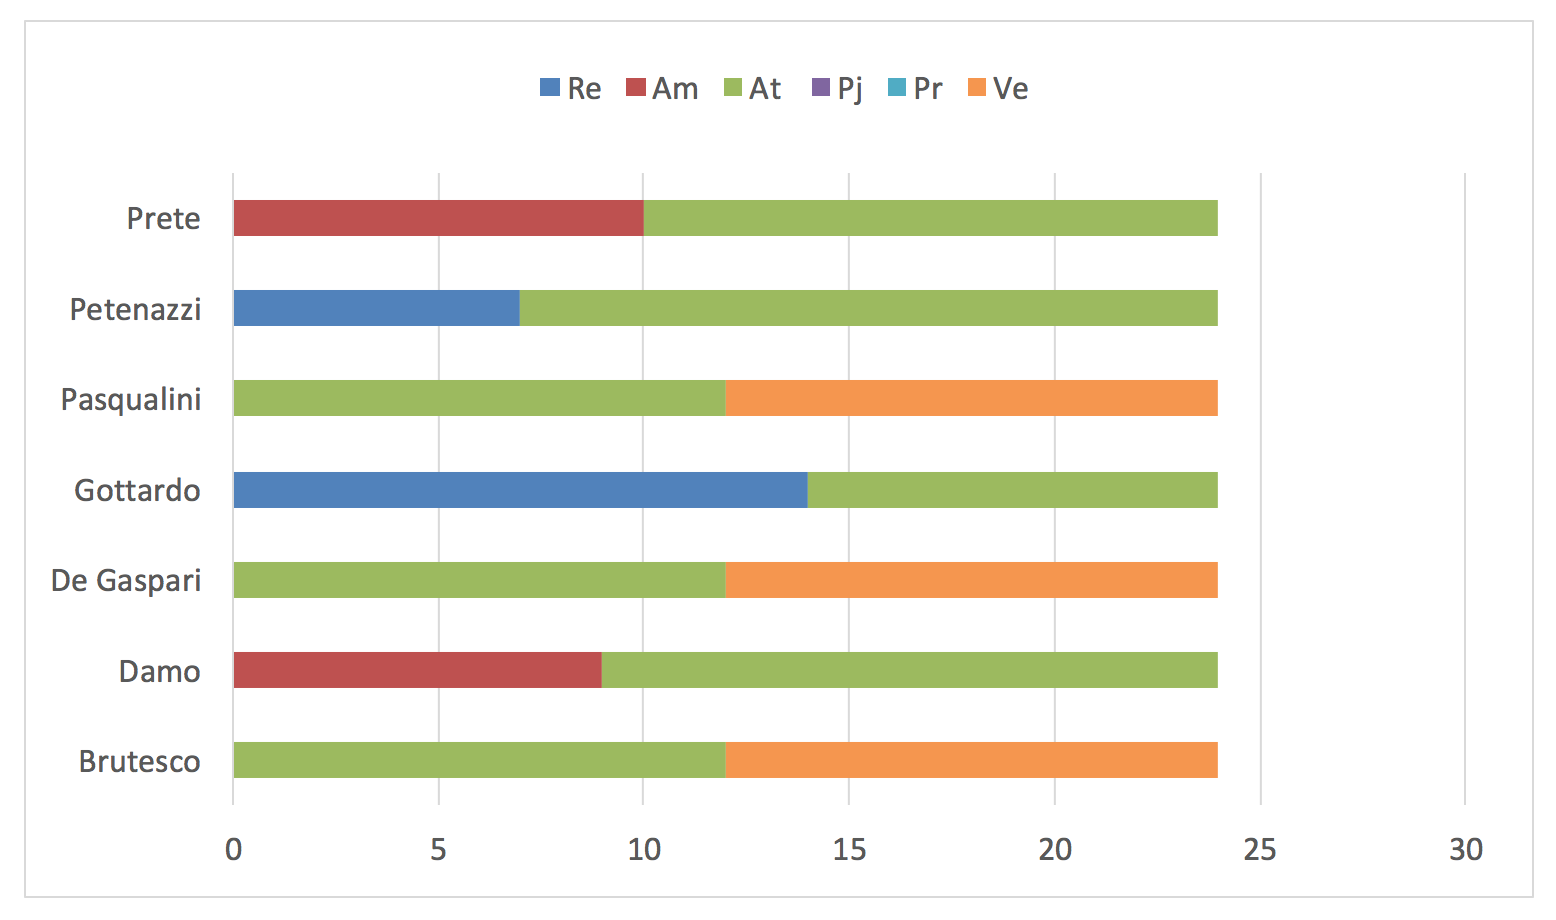
\includegraphics[scale=0.35]{img/h_An}
									\caption{Grafico del preventivo orario - Periodo: An}  \label{fig:h_An"} 		\end{figure}


%-----------------------------------------------------------------
			\begin{figure}[H]
			\centering
			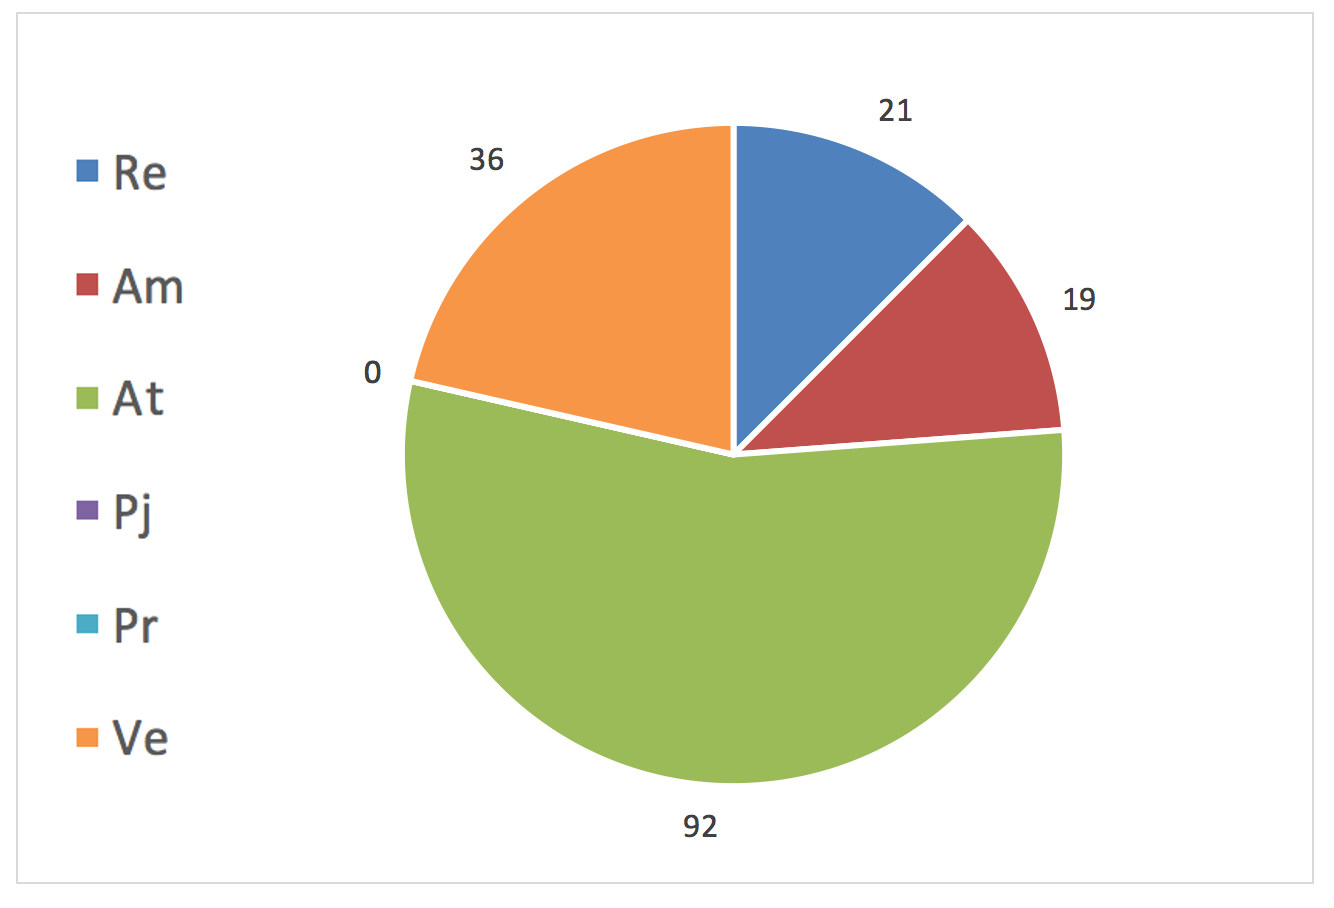
\includegraphics[scale=0.30]{img/h_r_An}
			\caption{Grafico del preventivo orario per ruolo - Periodo: An}
			\label{fig:h_r_An"}
			\end{figure}

		\newpage
			\paragraph{Preventivo economico}
		Le ore di questo periodo sono considerate solamente come ore di investimento e quindi non rendicontate.\\
%-----------------------------------------------------------------


							\begin{table}[H] \begin{center} \begin{tabular}{llllllll}
							\toprule
								&	\textbf{Re}	&	\textbf{Am}	&	\textbf{At}	&	\textbf{Pj}	&	\textbf{Pr}	&	\textbf{Ve}	&	\textbf{Tot}\\
							\midrule
							Tot in ore	&	21	&	19	&	92	&	0	&	0	&	36	&	168	 \\
							Tot. in €	&	 €     630,00 	 & 	 €  380,00 	 & 	 €  2.300,00 	 & 	 €           -   	 & 	 €               -   	 & 	 €  540,00 	 & 	 €        3.850,00 	 \\
							\bottomrule
							\end{tabular} \end{center} \caption{Prospetto economico - Periodo:
							An
							}\label{tab:s_An} \end{table}		\begin{figure}[H]  \centering  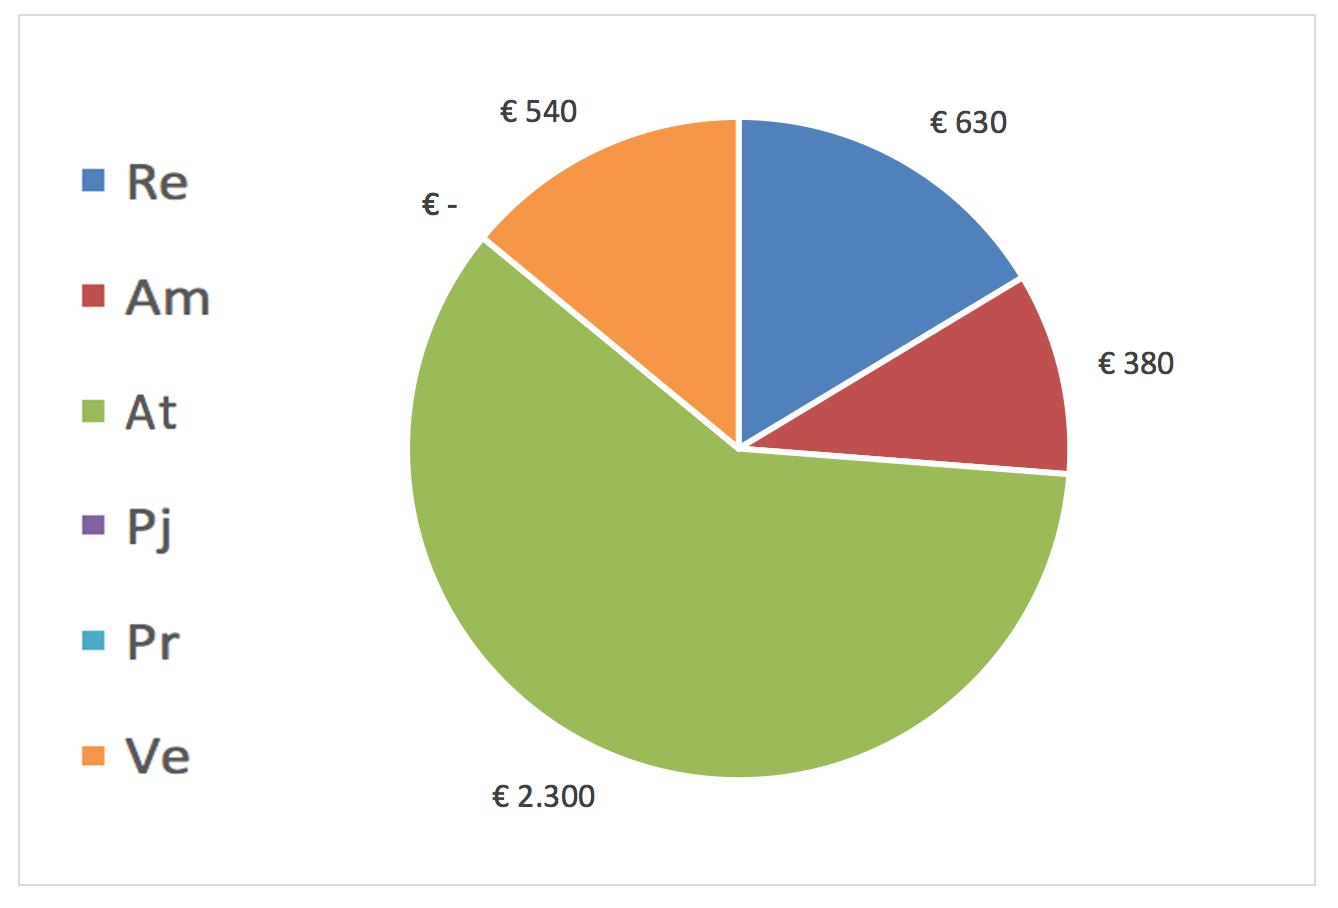
\includegraphics[scale=0.40]{img/s_An}
									\caption{Grafico del preventivo economico - Periodo: An}  \label{fig:s_An"} 		\end{figure}


%-----------------------------------------------------------------
		\newpage
		\subsubsection {Periodo: Pl - Progettazione logica}
		\paragraph{Preventivo orario}
%-----------------------------------------------------------------


							\begin{table}[H] \begin{center} \begin{tabular}{llllllll}
							\toprule
							\textbf{Nominativo}	&	\textbf{Re}	&	\textbf{Am}	&	\textbf{At}	&	\textbf{Pj}	&	\textbf{Pr}	&	\textbf{Ve}	&	\textbf{Tot}\\
							\midrule
							Brutesco	&	5	&	-	&	-	&	21	&	-	&	-	&	26	 \\
							Damo	&	5	&	-	&	-	&	30	&	-	&	-	&	35	 \\
							De Gaspari	&	-	&	-	&	-	&	10	&	-	&	16	&	26	 \\
							Gottardo	&	-	&	-	&	-	&	10	&	-	&	16	&	26	 \\
							Pasqualini	&	-	&	5	&	5	&	16	&	-	&	-	&	26	 \\
							Petenazzi	&	-	&	4	&	5	&	17	&	-	&	-	&	26	 \\
							Prete	&	-	&	-	&	-	&	10	&	-	&	16	&	26	 \\
							\midrule
							Tot in ore	&	10	&	9	&	10	&	114	&	0	&	48	&	191	 \\



							\bottomrule
							\end{tabular} \end{center} \caption{Prospetto orario - Periodo:
							Pl
							}\label{tab:h_Pl} \end{table}		\begin{figure}[H]  \centering  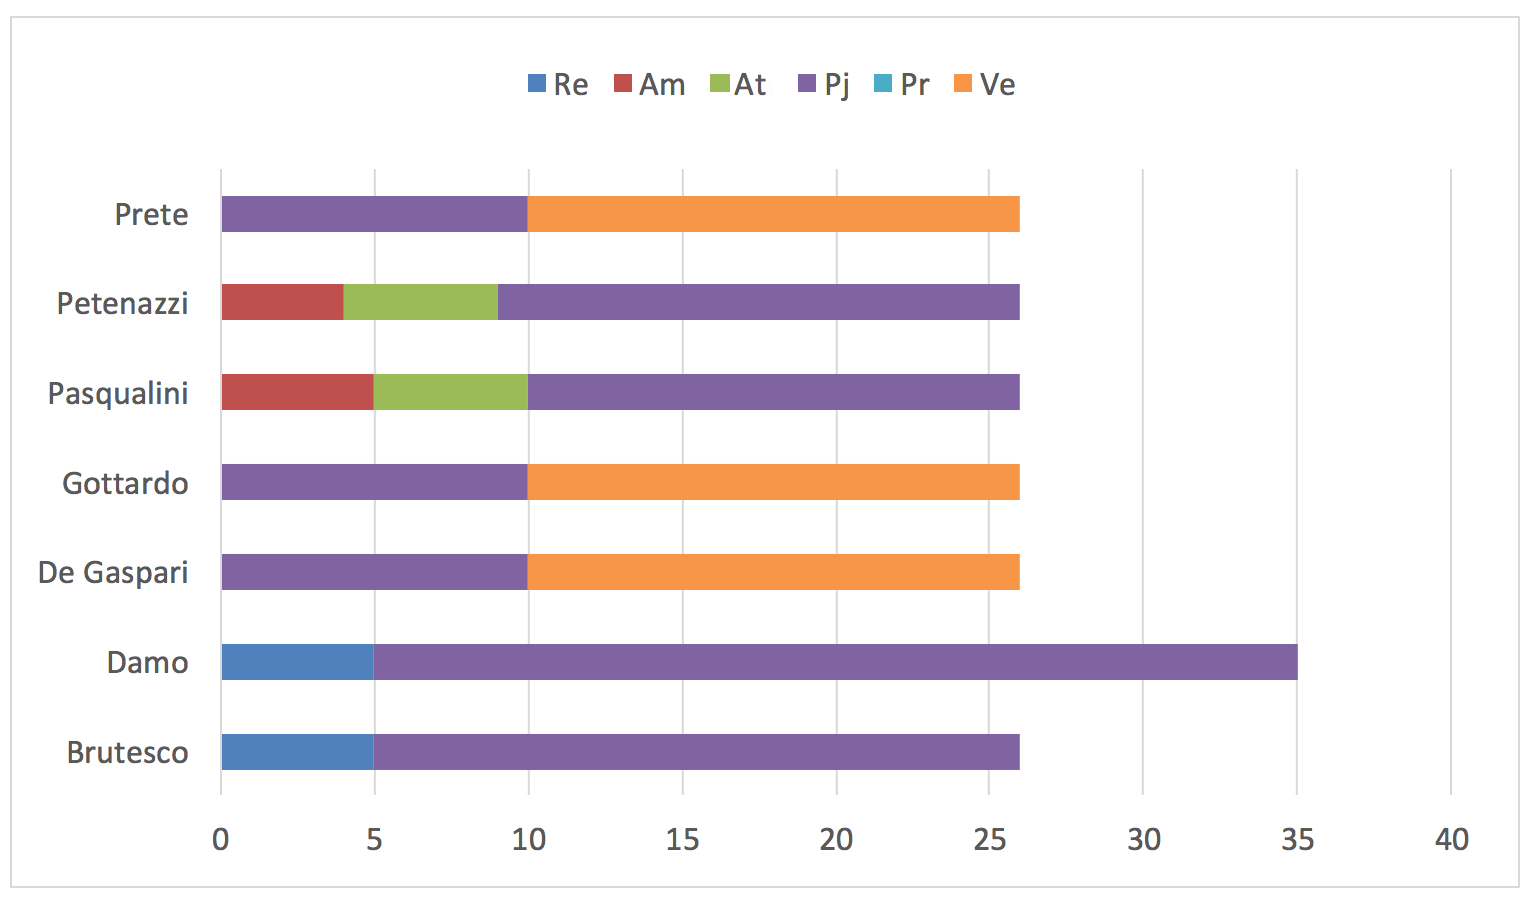
\includegraphics[scale=0.43]{img/h_Pl}
									\caption{Grafico del preventivo orario - Periodo: Pl}  \label{fig:h_Pl"} 		\end{figure}


%-----------------------------------------------------------------

			\begin{figure}[H]
			\centering
			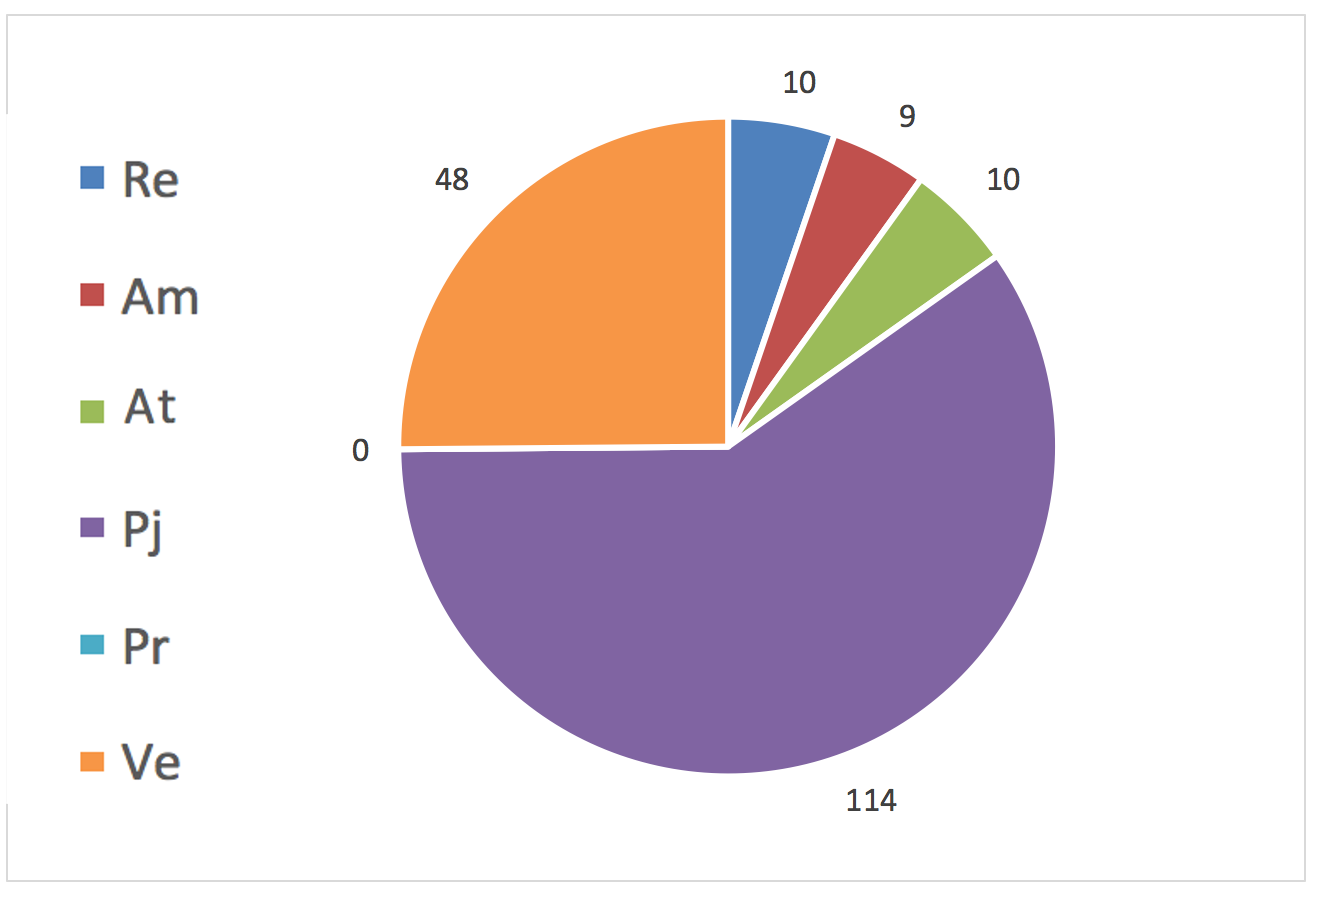
\includegraphics[scale=0.35]{img/h_r_Pl}
			\caption{Grafico del preventivo orario per ruolo - Periodo: Pl}
			\label{fig:h_r_Pl"}
			\end{figure}

			\newpage
			\paragraph{Preventivo economico}
			Il preventivo economico viene illustrato dalla tabella seguente. Le ore riportate sono tutte rendicontate.\\

%-----------------------------------------------------------------

							\begin{table}[H] \begin{center} \begin{tabular}{llllllll}
							\toprule
								&	\textbf{Re}	&	\textbf{Am}	&	\textbf{At}	&	\textbf{Pj}	&	\textbf{Pr}	&	\textbf{Ve}	&	\textbf{Tot}\\

							\midrule
							Tot in ore	&	10	&	9	&	10	&	114	&	0	&	48	&	191	 \\


							Tot in €	&	 €     300 	 & 	 €      180 	 & 	 €     250 	 & 	 €  2.508 	 & 	 €        -   	 & 	 €     720 	 & 	 €     3.958 	 \\
							\bottomrule
							\end{tabular} \end{center} \caption{Prospetto economico - Periodo:
							Pl
							}\label{tab:s_Pl} \end{table}


							\begin{figure}[H]  \centering  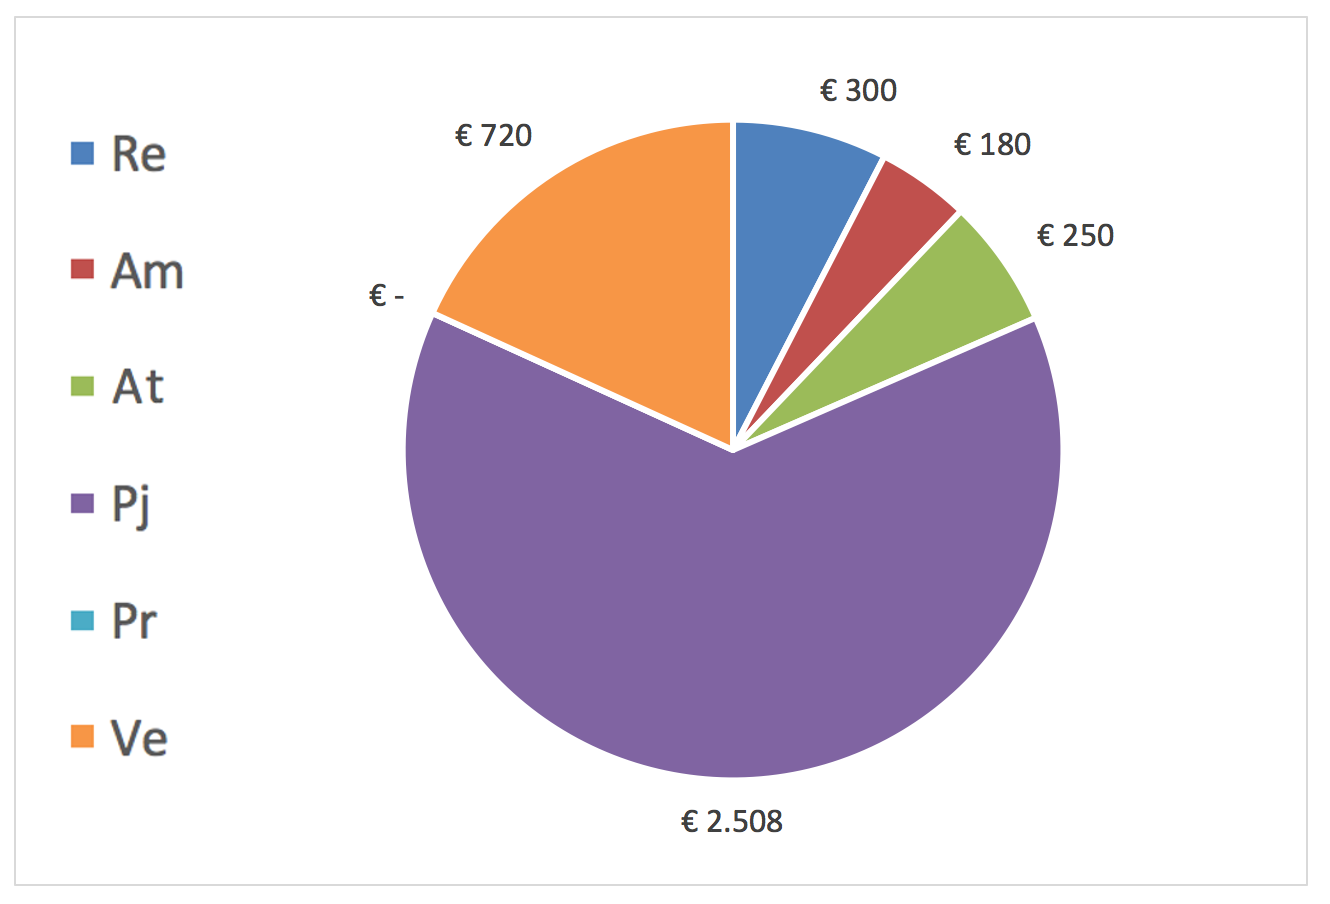
\includegraphics[scale=0.40]{img/s_Pl}
									\caption{Grafico del preventivo economico - Periodo: 								Pl	}  \label{fig:s_Pl"} 		\end{figure}
%-----------------------------------------------------------------
		\newpage
		\subsubsection {Periodo: PCV - Progettazione di dettaglio Codifica Validazione}
		\paragraph{Preventivo orario}
%-----------------------------------------------------------------

							\begin{table}[H] \begin{center} \begin{tabular}{llllllll}
							\toprule
							\textbf{Nominativo}	&	\textbf{Re}	&	\textbf{Am}	&	\textbf{At}	&	\textbf{Pj}	&	\textbf{Pr}	&	\textbf{Ve}	&	\textbf{Tot}\\
							\midrule
							Brutesco	&	-	&	4	&	-	&	5	&	15	&	29	&	53	 \\ 
							Damo	&	-	&		&	-	&	9	&	22	&	39	&	70	 \\ 
							De Gaspari	&	10	&	-	&	-	&	8	&	25	&	13	&	56	 \\ 
							Gottardo	&	-	&	6	&	-	&	28	&	22	&	-	&	56	 \\ 
							Pasqualini	&	-	&	4	&	-	&	29	&	16	&	7	&	56	 \\ 
							Petenazzi	&	-	&	5	&	-	&	12	&	20	&	19	&	56	 \\ 
							Prete	&	10	&	-	&	-	&	6	&	21	&	16	&	53	 \\ 
							\midrule															
							Tot in ore	&	20	&	19	&	0	&	97	&	141	&	123	&	400	 \\ 
							


							\bottomrule
							\end{tabular} \end{center} \caption{Prospetto orario - Periodo:
							PCV
							}\label{tab:h_PCV} \end{table}		\begin{figure}[H]  \centering  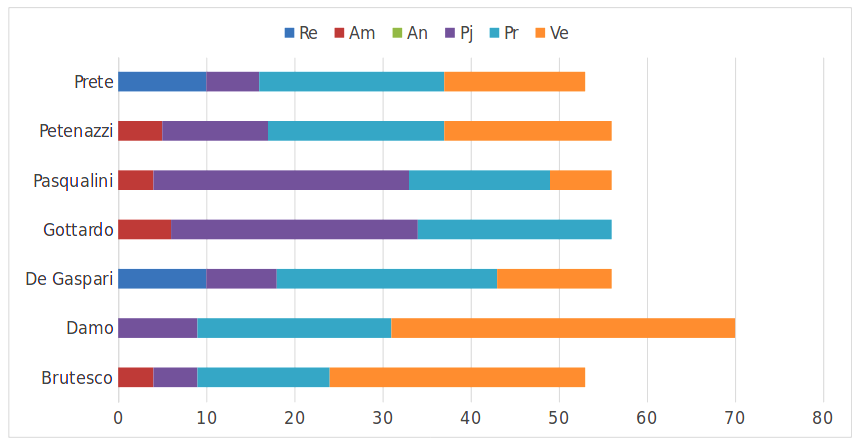
\includegraphics[scale=0.37]{img/h_PCV}
									\caption{Grafico del preventivo orario - Periodo: 								PCV	}  \label{fig:h_PCV} \end{figure}

%-----------------------------------------------------------------
			\begin{figure}[H]
			\centering
			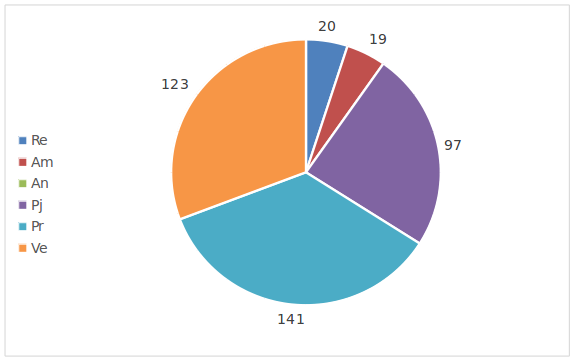
\includegraphics[scale=0.42]{img/h_r_PCV}
			\caption{Grafico del preventivo orario per ruolo - Periodo: PCV}
			\label{fig:h_r_PCV"}
			\end{figure}

			\newpage
			\paragraph{Preventivo economico}
			Il preventivo economico viene illustrato dalla tabella seguente. Le ore riportate sono tutte rendicontate.\\
%-----------------------------------------------------------------

							\begin{table}[H] \begin{center} \begin{tabular}{llllllll}
							\toprule
								&	\textbf{Re}	&	\textbf{Am}	&	\textbf{At}	&	\textbf{Pj}	&	\textbf{Pr}	&	\textbf{Ve}	&	\textbf{Tot}\\

							\midrule
							Tot in ore	&	20	&	19	&	0	&	97	&	141	&	123	&	400	 \\ 
							Tot in €	&	 € 600 	 & 	 € 380 	 & 	 € -   	 & 	 € 2.134 	 & 	 € 2.115 	 & 	 € 1.845 	 & 	 € 7.074 	 \\ 
							\bottomrule
							\end{tabular} \end{center} \caption{Prospetto economico - Periodo:
							PCV
							}\label{tab:s_PCV} \end{table}		\begin{figure}[H]  \centering  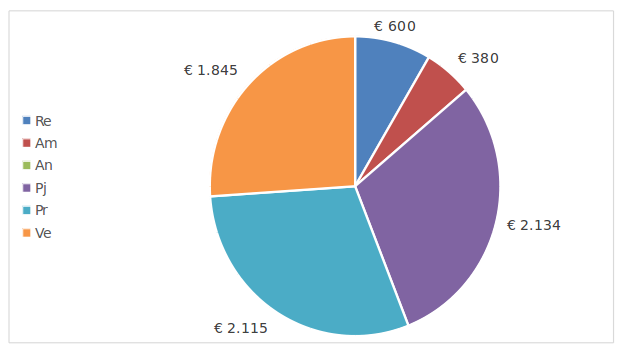
\includegraphics[scale=0.40]{img/s_PCV.png}
									\caption{Grafico del preventivo economico - Periodo: 								PCV	}  \label{fig:s_PCV} \end{figure}

%-----------------------------------------------------------------
		\newpage
		\subsubsection {Periodo: Va - Validazione}
		\paragraph{Preventivo orario}
%-----------------------------------------------------------------

							\begin{table}[H] \begin{center} \begin{tabular}{llllllll}
							\toprule
							\textbf{Nominativo}		&	\textbf{Re}	&	\textbf{Am}	&	\textbf{At}	&	\textbf{Pj}	&	\textbf{Pr}	&	\textbf{Ve}	&	\textbf{Tot}\\
							\midrule
							Brutesco	&	-	&	-	&	-	&	-	&	6	&	20	&	26	 \\
							Damo	&	-	&	-	&	-	&	-	&	-	&	-	&	0	 \\
							De Gaspari	&	-	&	10	&	-	&	-	&	-	&	13	&	23	 \\
							Gottardo	&	-	&	-	&	-	&	-	&	6	&	17	&	23	 \\
							Pasqualini	&	13	&	-	&	-	&	-	&	-	&	10	&	23	 \\
							Petenazzi	&	-	&	-	&	-	&	-	&	7	&	16	&	23	 \\
							Prete	&	-	&	-	&	-	&	-	&	11	&	15	&	26	 \\
							\midrule
							Tot in ore	&	13	&	10	&	0	&	0	&	30	&	91	&	144	 \\


							\bottomrule
							\end{tabular} \end{center} \caption{Prospetto orario - Periodo:
							Va
							}\label{tab:h_Va} \end{table}		\begin{figure}[H]  \centering  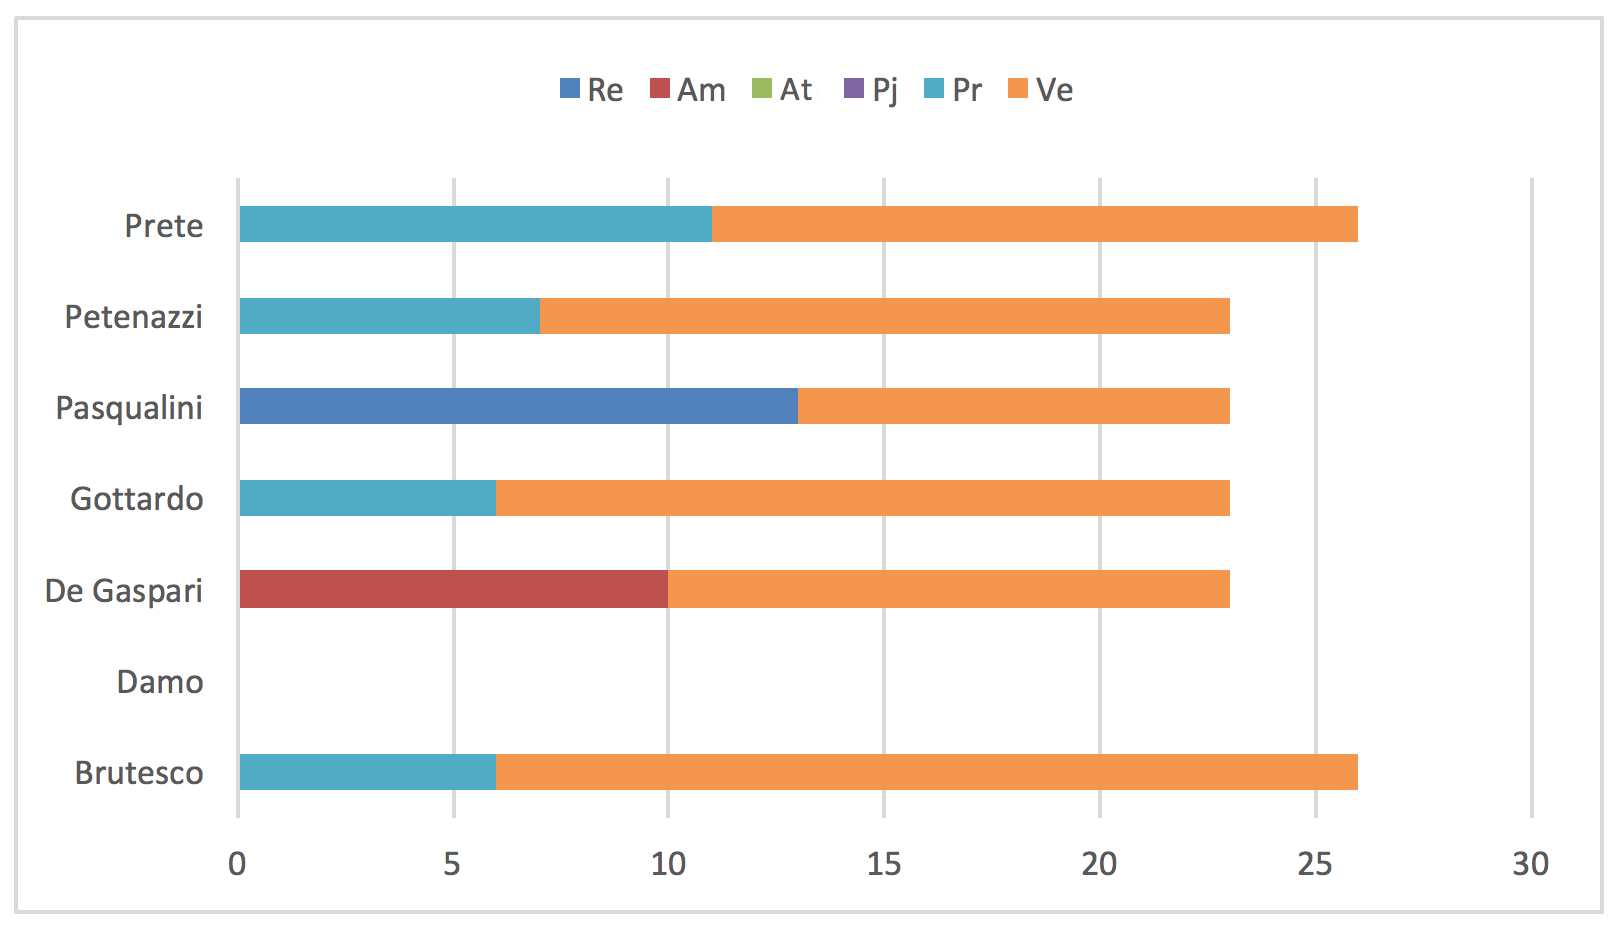
\includegraphics[scale=0.42]{img/h_Va}
									\caption{Grafico del preventivo orario - Periodo: 								Va	}  \label{fig:h_Va} \end{figure}
%-----------------------------------------------------------------
			\begin{figure}[H]
			\centering
			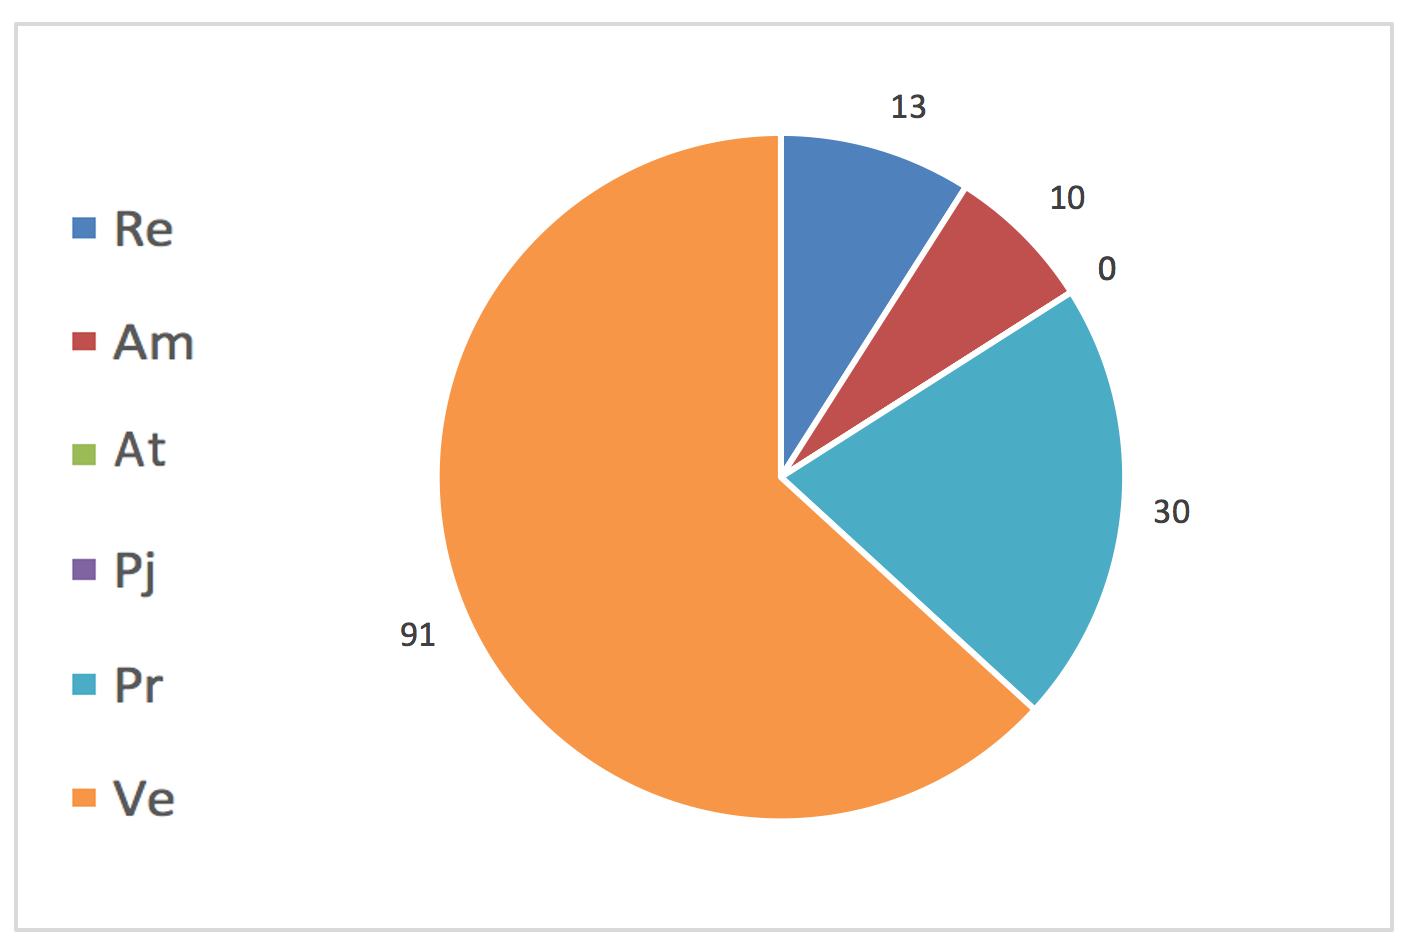
\includegraphics[scale=0.32]{img/h_r_Va}
			\caption{Grafico del preventivo orario per ruolo - Periodo: Va}
			\label{fig:Va"}
			\end{figure}

			\newpage
			\paragraph{Preventivo economico}
			Il preventivo economico viene illustrato dalla tabella seguente. Le ore riportate sono tutte rendicontate.\\

%-----------------------------------------------------------------

							\begin{table}[H] \begin{center} \begin{tabular}{llllllll}
							\toprule
								&	\textbf{Re}	&	\textbf{Am}	&	\textbf{At}	&	\textbf{Pj}	&	\textbf{Pr}	&	\textbf{Ve}	&	\textbf{Tot}\\

							\midrule
							Tot in ore	&	13	&	10	&	0	&	0	&	30	&	91	&	144	 \\


							Tot in €	&	 €     390 	 & 	 €      200 	 & 	 €         -   	 & 	 €         -   	 & 	 €    450 	 & 	 €  1.365 	 & 	 €     2.405 	 \\
							\bottomrule
							\end{tabular} \end{center} \caption{Prospetto economico - Periodo:
							Va
							}\label{tab:s_Va} \end{table}		\begin{figure}[H]  \centering  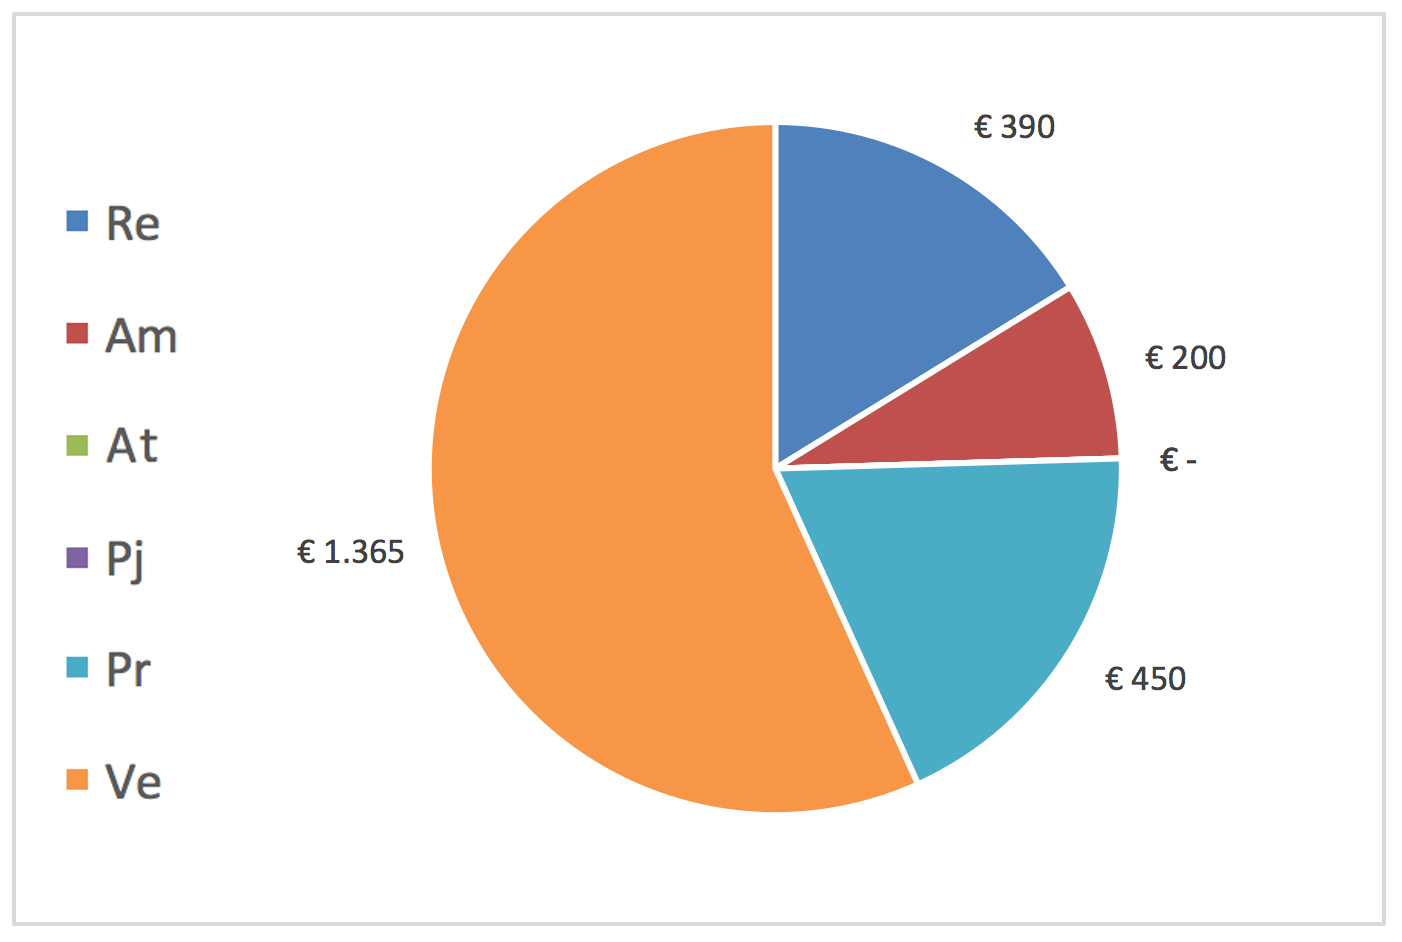
\includegraphics[scale=0.40]{img/s_Va}
									\caption{Grafico del preventivo economico - Periodo: 								Va	}  \label{fig:s_Va	} \end{figure}

%-----------------------------------------------------------------
	\newpage
	\subsection {Totale non rendicontato}
		\subsubsection {Preventivo orario}
		Si stima inoltre che ogni membro del \glo{Gruppo}{gruppo} dedicherà per ogni ruolo un numero di ore non rendicontate di investimento pari a:\\
		\begin{table}[H] \begin{center} \begin{tabular}{lllllll}
		\toprule
			Re	&	Am	&	An	&	Pj	&	Pr	&	Ve	&	Tot	 \\
		\midrule
			2	&	3	&	2	&	2	&	2	&	2	&	13	 \\
		\bottomrule
		\end{tabular} \end{center}
		\caption{Ulteriori ore non rendicontate}
		\label{tab:h_ulteriori}
        \end{table}\mbox{}\\

		Quindi, durante l'intero arco dello sviluppo del progetto, le ore non rendicontate ammontano a:\\
%-----------------------------------------------------------------

							\begin{table}[H] \begin{center} \begin{tabular}{llllllll}
							\toprule
							\textbf{Nominativo}	&	\textbf{Re}	&	\textbf{Am}	&	\textbf{At}	&	\textbf{Pj}	&	\textbf{Pr}	&	\textbf{Ve}	&	\textbf{Tot}\\
							\midrule
							Brutesco	&	2	&	3	&	14	&	2	&	2	&	14	&	37	 \\
							Damo		&	2	&	12	&	17	&	2	&	2	&	2	&	37	 \\
							De Gaspari	&	2	&	3	&	14	&	2	&	2	&	14	&	37	 \\
							Gottardo	&	16	&	3	&	12	&	2	&	2	&	2	&	37	 \\
							Pasqualini	&	2	&	3	&	14	&	2	&	2	&	14	&	37	 \\
							Petenazzi	&	9	&	3	&	19	&	2	&	2	&	2	&	37	 \\
							Prete		&	2	&	13	&	16	&	2	&	2	&	2	&	37	 \\
							\midrule
							Tot in ore	&	35	&	40	&	106	&	14	&	14	&	50	&	259	 \\
							\bottomrule
							\end{tabular} \end{center}
							\caption{Prospetto riassuntivo delle ore non rendicontate}
							\label{tab:h_TotaleNonRendicontato} \end{table}\mbox{}\\

							\begin{figure}[H]  \centering
							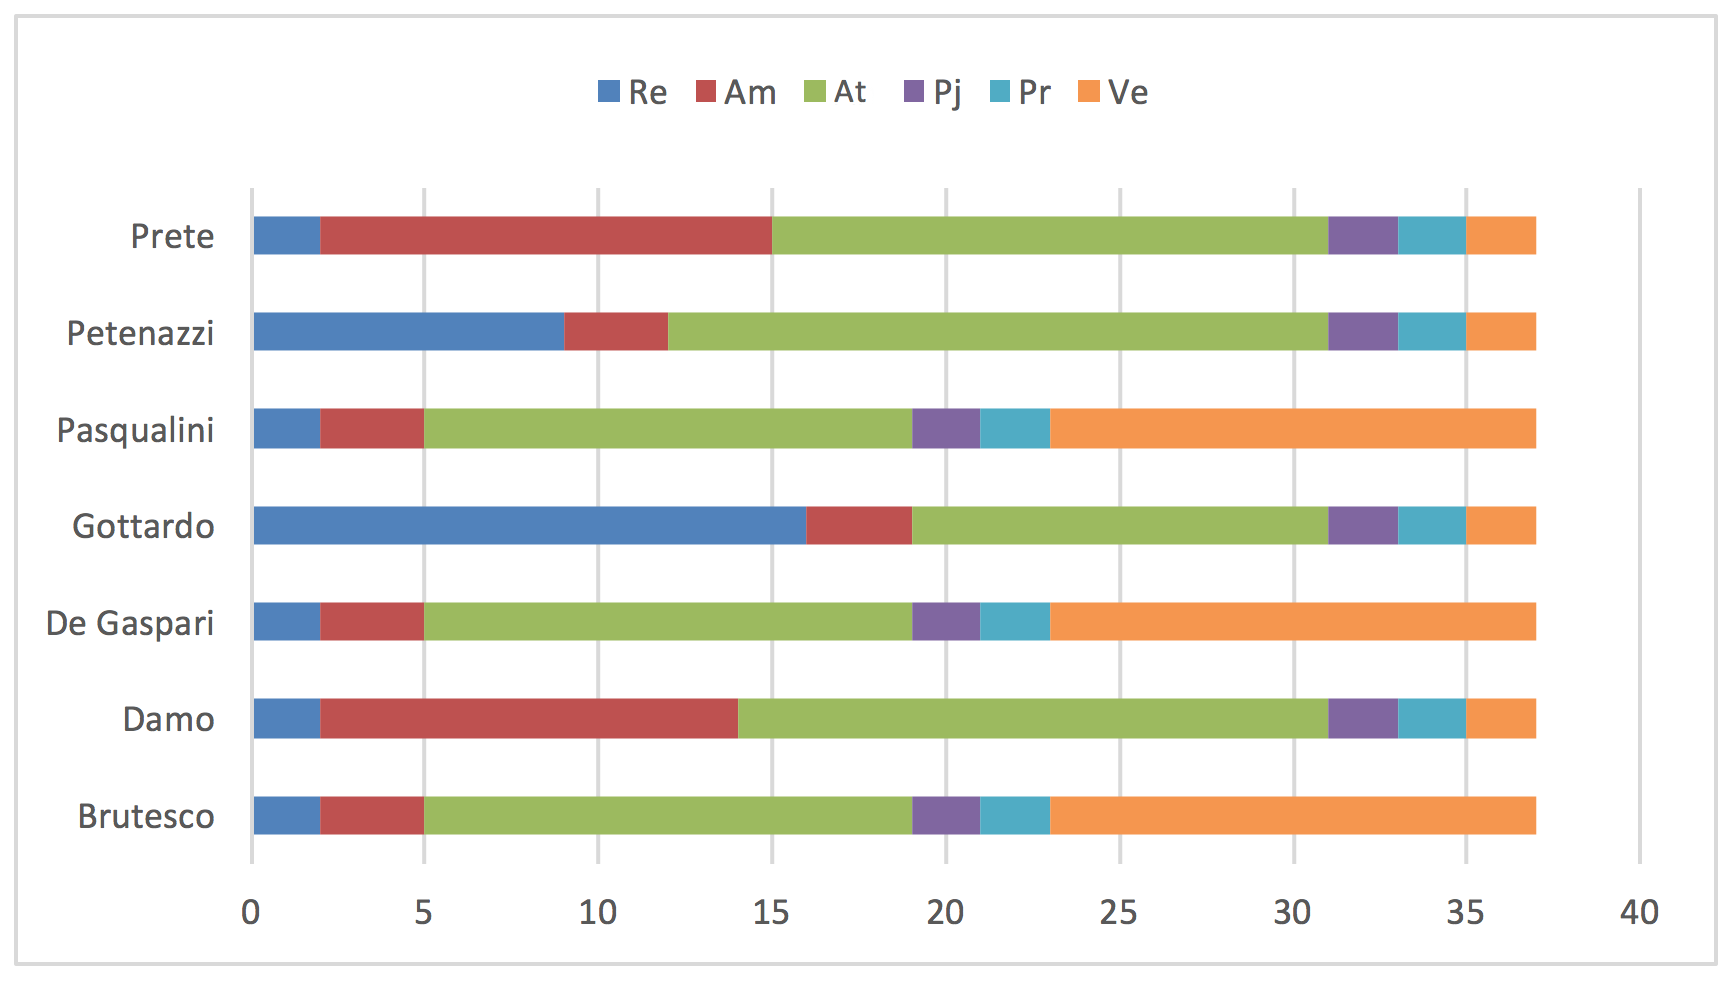
\includegraphics[width=\textwidth]{img/h_NonRend}
							\caption{Grafico riassuntivo delle ore non rendicontate}
							\label{fig:h_non_rend"} 		\end{figure}
%-----------------------------------------------------------------
			\begin{figure}[H]
			\centering
			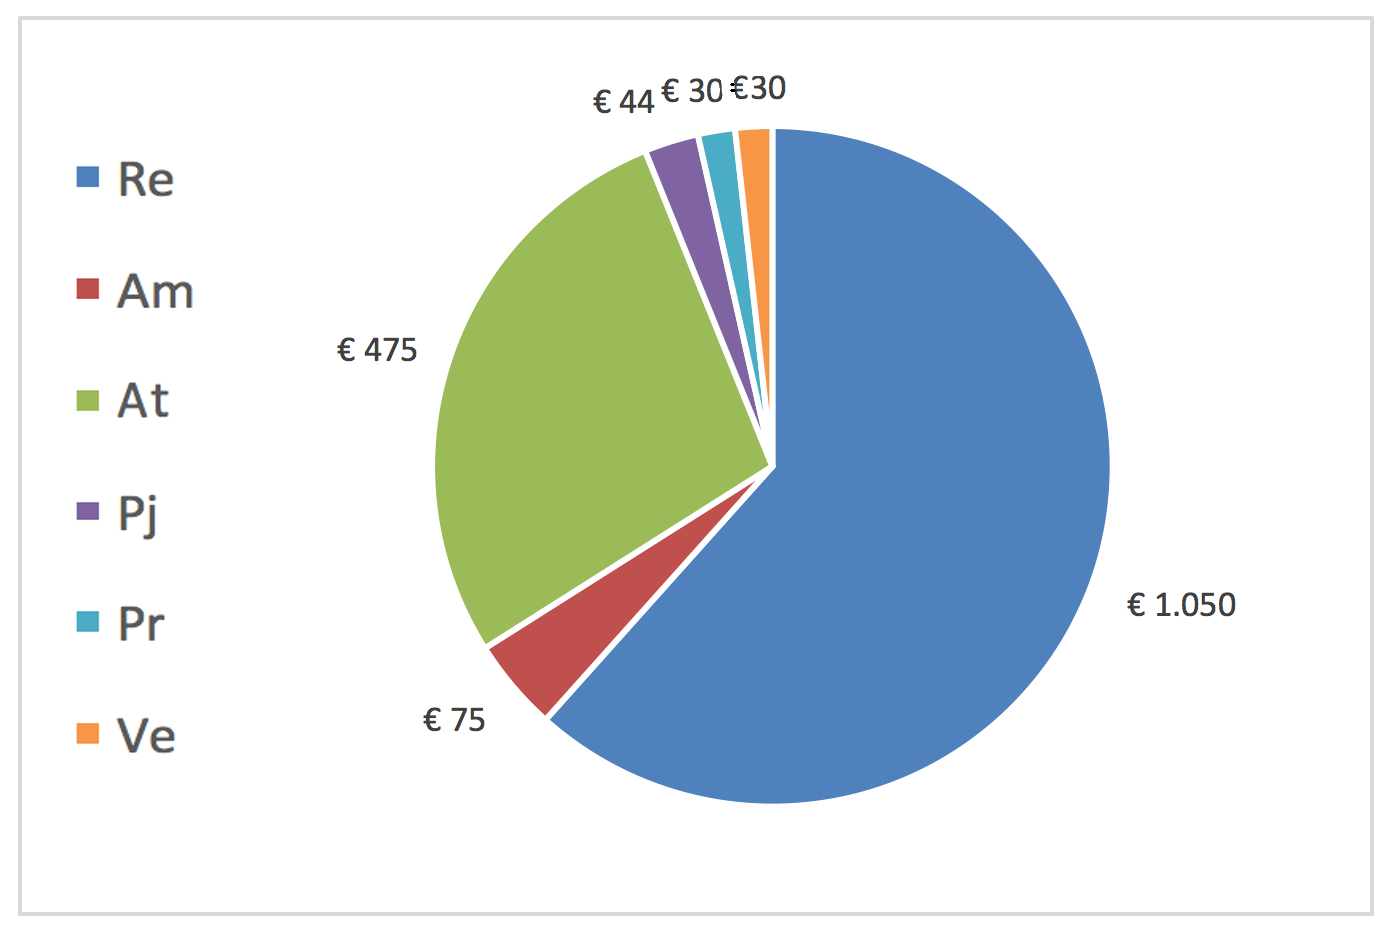
\includegraphics[scale=0.40]{img/h_r_TotaleNonRendicontato}
			\caption{Grafico del preventivo orario per ruolo - Totale non rendicontato}
			\label{fig:Totale non rendicontato"}
			\end{figure}
%-----------------------------------------------------------------
			\begin{figure}[H]
			\centering
			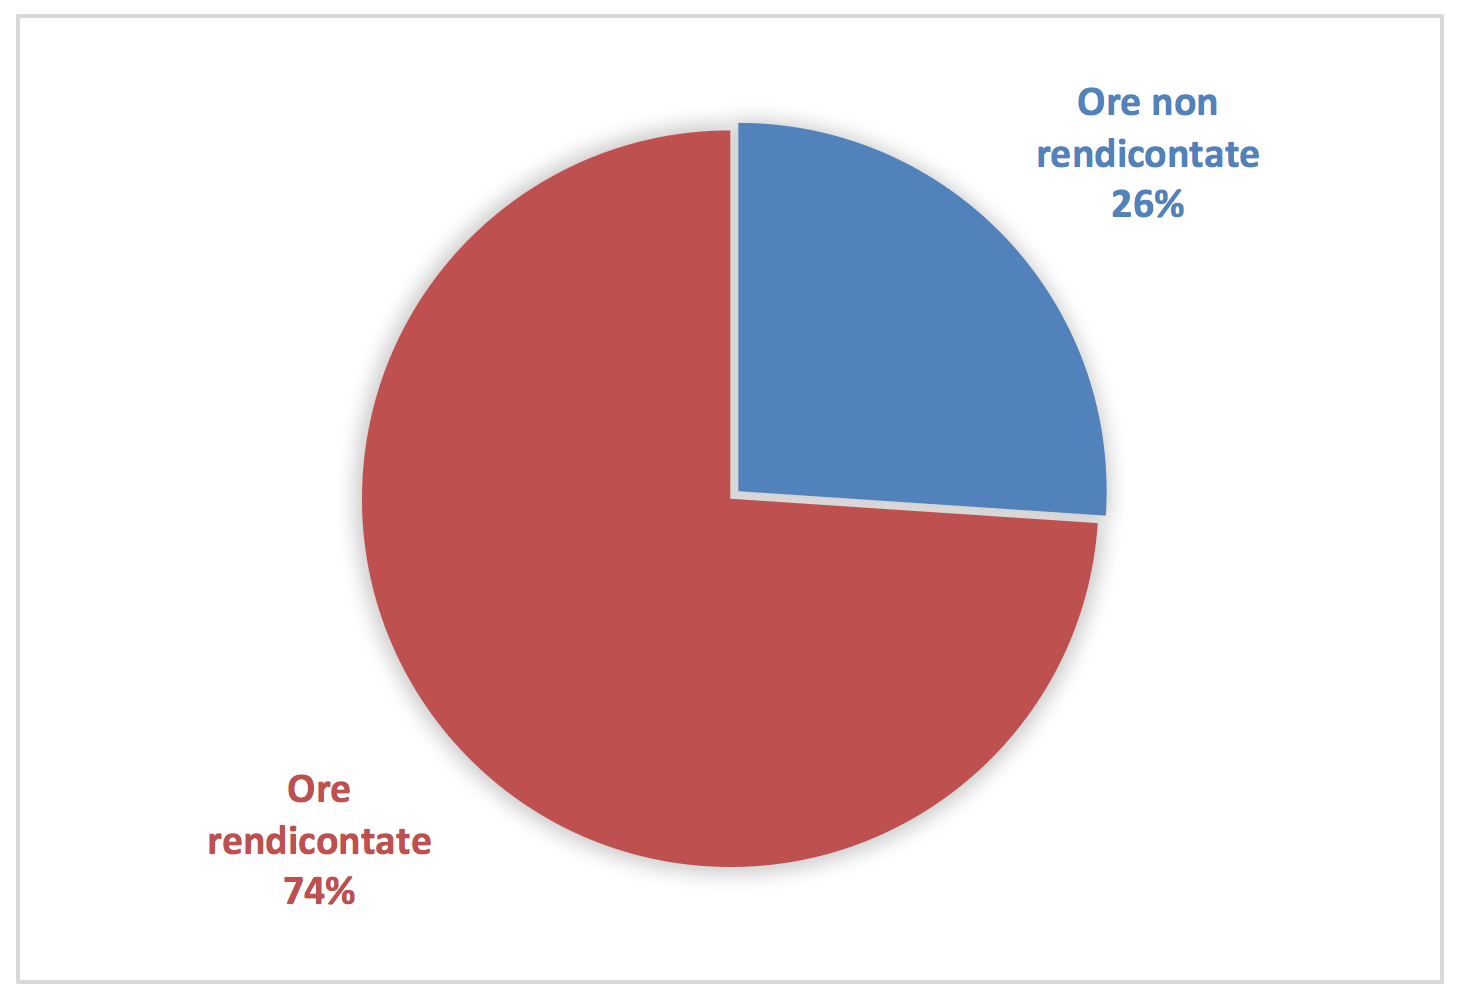
\includegraphics[scale=0.40]{img/incidenza}
			\caption{Incidenza delle ore non rendicontate sul totale delle ore complessivo}
			\label{fig:incidenza}
			\end{figure}
%-----------------------------------------------------------------
			\newpage
			\subsubsection {Preventivo economico}
%-----------------------------------------------------------------
			\begin{table}[H] \begin{center} \begin{tabular}{llllllll}
			\toprule
				&	\textbf{Re}	&	\textbf{Am}	&	\textbf{At}	&	\textbf{Pj}	&	\textbf{Pr}	&	\textbf{Ve}	&	\textbf{Tot}\\

			\midrule
			Tot in ore	&	35	&	40	&	106	&	14	&	14	&	50	&	259	 \\


			Tot in €	&	 €        1.050 	 & 	 €        800 	 & 	 €        2.650 	 & 	 €        308 	 & 	 €            210 	 & 	 €        750 	 & 	 €              5.768 	 \\
			\bottomrule
			\end{tabular} \end{center} \caption{Prospetto economico -
			Totale non rendicontato
			}\label{tab:s_TotaleNonRendicontato_prev} \end{table}
%-----------------------------------------------------------------
			\begin{figure}[H]
			\centering
			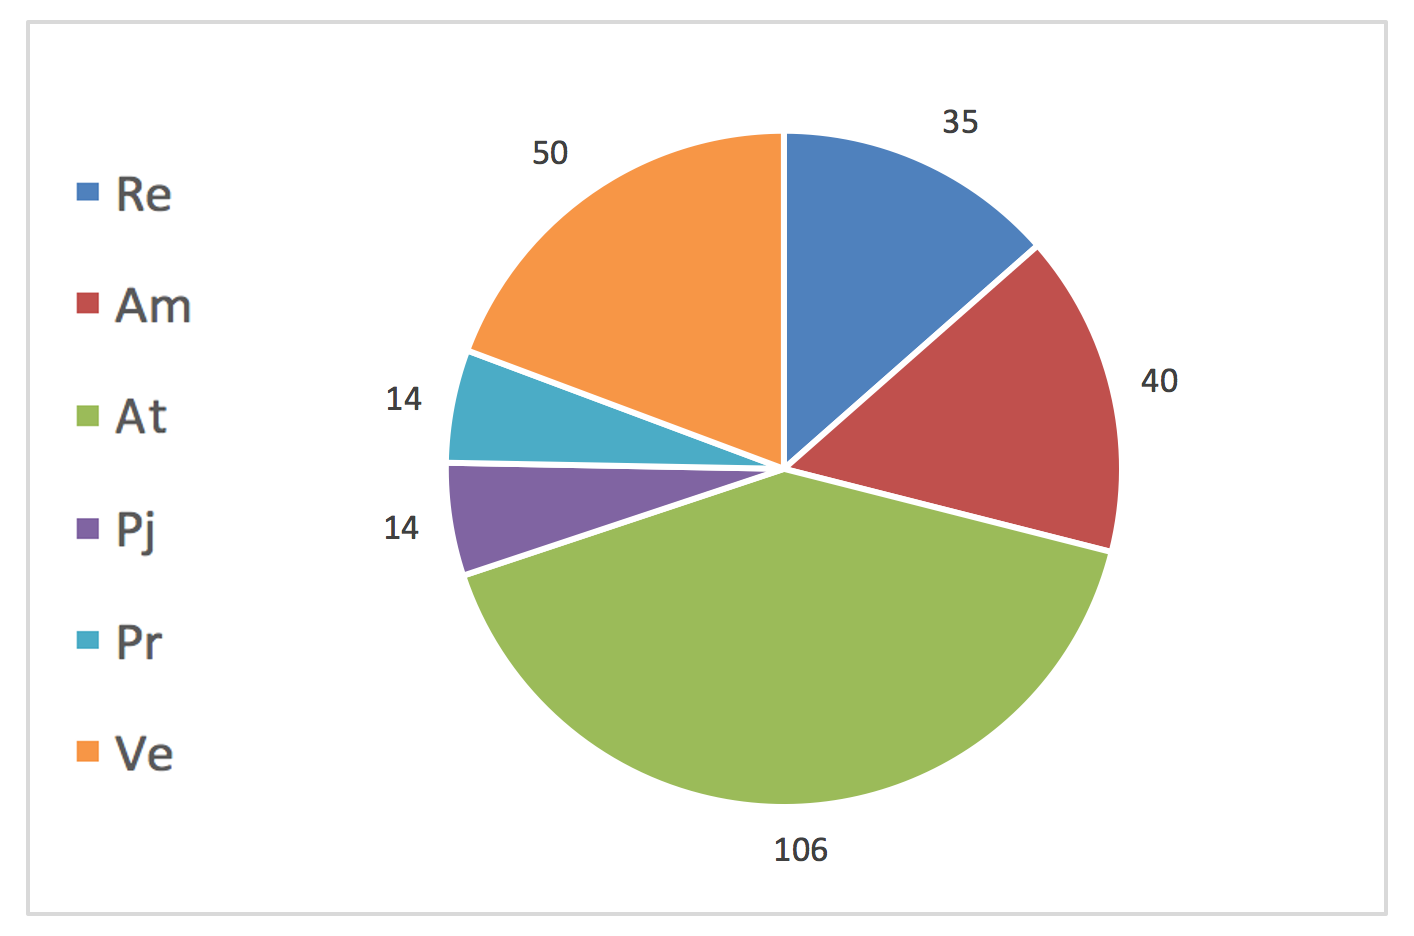
\includegraphics[scale=0.40]{img/s_TotaleNonRendicontato}
			\caption{Grafico del preventivo economico per ruolo - Totale non rendicontato}
			\label{fig:TotaleNonRendicontato}
			\end{figure}
%-----------------------------------------------------------------
		\newpage
		\subsection {Totale complessivo}
				\subsubsection {Preventivo orario}
		Durante l'intero arco dello sviluppo del progetto, includendo anche le ore non rendicontate, i membri del gruppo ricopriranno i vari ruoli secondo la seguente suddivisione:\\
%-----------------------------------------------------------------

								\begin{table}[H] \begin{center} \begin{tabular}{llllllll}
								\toprule
								\textbf{Nominativo}	&	\textbf{Re}	&	\textbf{Am}	&	\textbf{At}	&	\textbf{Pj}	&	\textbf{Pr}	&	\textbf{Ve}	&	\textbf{Tot}\\
								\midrule
								Brutesco	&	7	&	7	&	14	&	28	&	23	&	63	&	142	 \\
								Damo	&	7	&	12	&	17	&	41	&	24	&	41	&	142	 \\
								De Gaspari	&	12	&	13	&	14	&	20	&	27	&	56	&	142	 \\
								Gottardo	&	16	&	9	&	12	&	40	&	30	&	35	&	142	 \\
								Pasqualini	&	15	&	12	&	19	&	47	&	18	&	31	&	142	 \\
								Petenazzi	&	9	&	12	&	24	&	31	&	29	&	37	&	142	 \\
								Prete	&	12	&	13	&	16	&	18	&	34	&	49	&	142	 \\
								\midrule
								Tot in ore	&	78	&	78	&	116	&	225	&	185	&	312	&	994	 \\



								\bottomrule
								\end{tabular} \end{center} \caption{Prospetto orario -
								Totale complessivo
								}\label{tab:h_TotaleComplessivo} \end{table}\mbox{}\\
                        		\begin{figure}[H]  \centering  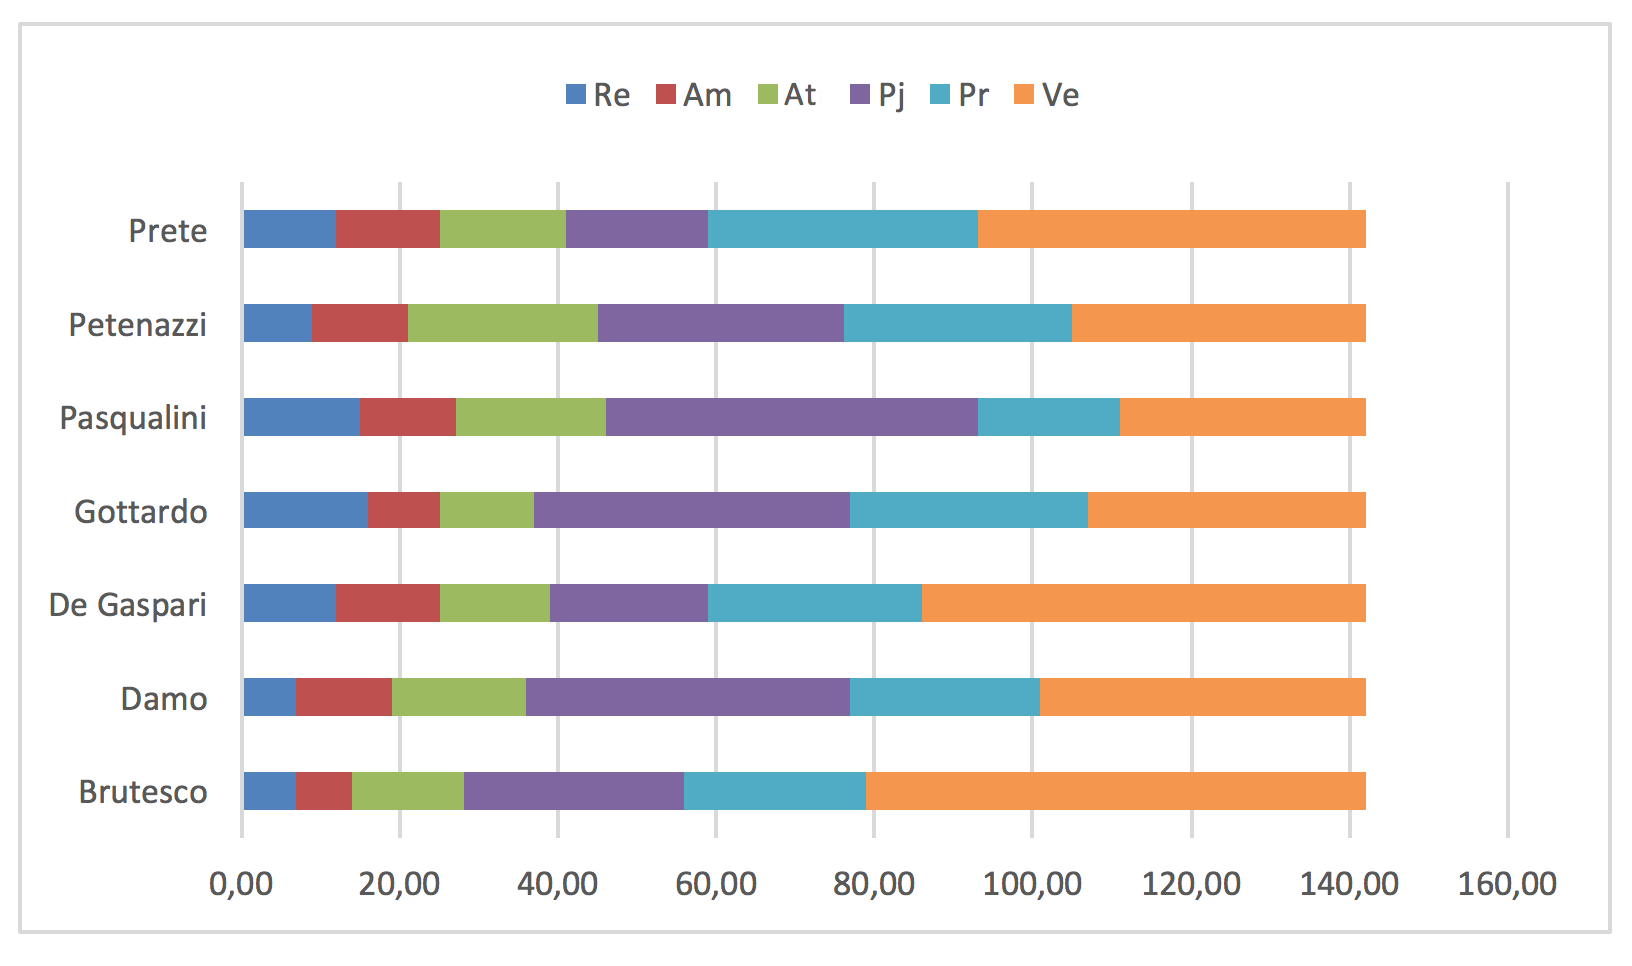
\includegraphics[scale=0.40]{img/h_Totale}
										\caption{Grafico del preventivo orario - 								Totale complessivo	}  \label{fig:h_TotaleComplessivo} \end{figure}
%-----------------------------------------------------------------
			\begin{figure}[H]
			\centering
			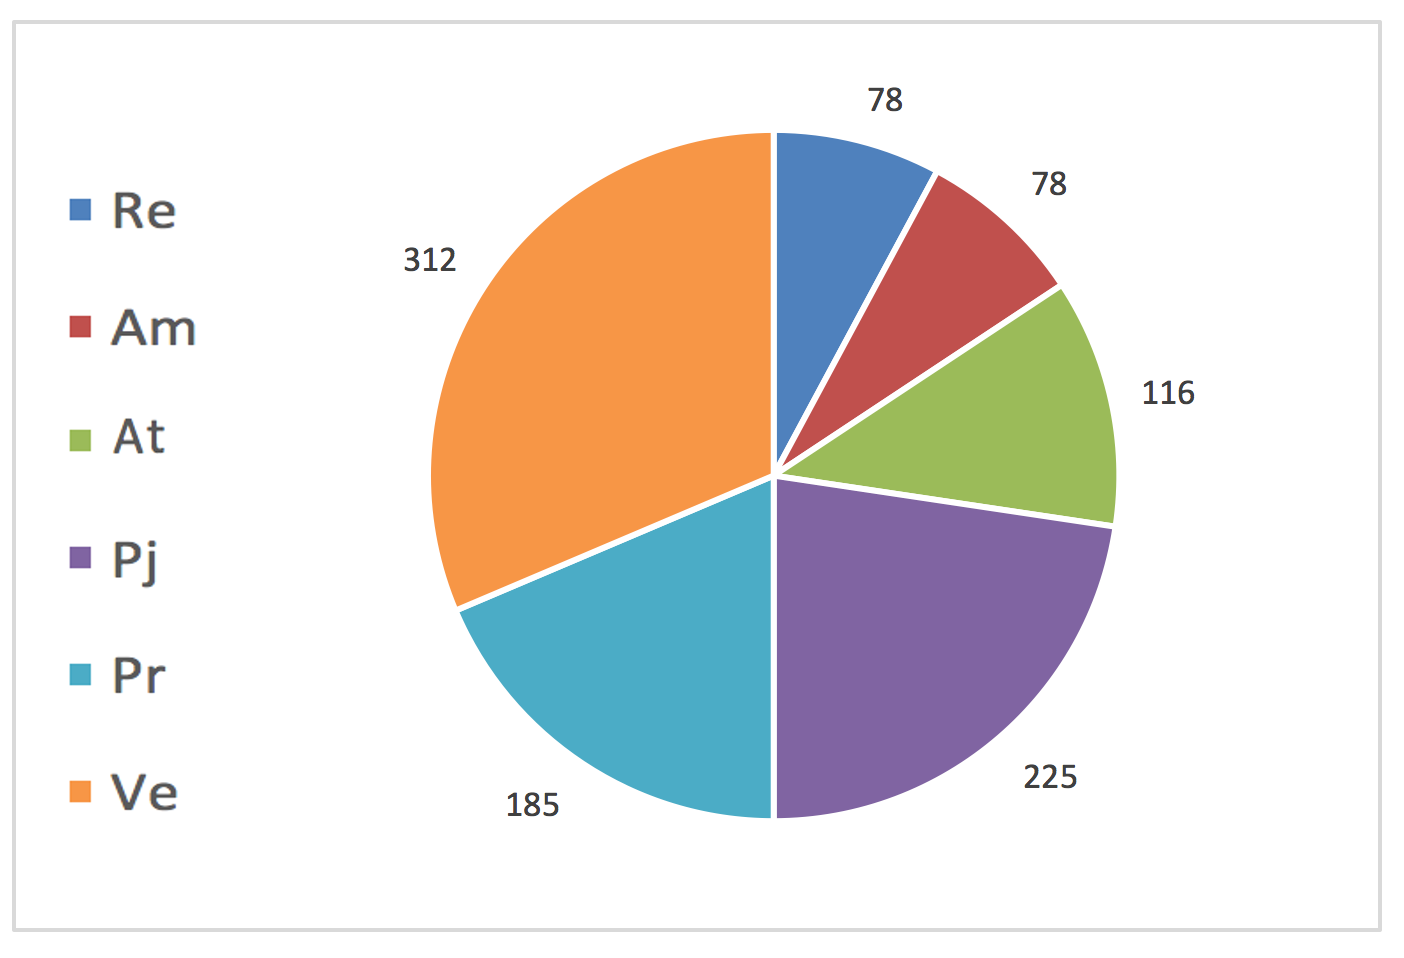
\includegraphics[scale=0.40]{img/h_r_Totale}
			\caption{Grafico del preventivo orario per ruolo - Totale complessivo}
			\label{fig:Totale complessivo orario}
			\end{figure}
					\newpage
					\subsubsection {Preventivo economico}
%-----------------------------------------------------------------

								\begin{table}[H] \begin{center} \begin{tabular}{llllllll}
								\toprule
									&	\textbf{Re}	&	\textbf{Am}	&	\textbf{At}	&	\textbf{Pj}	&	\textbf{Pr}	&	\textbf{Ve}	&	\textbf{Tot}\\
								\midrule
								Tot in ore	&	78	&	78	&	116	&	225	&	185	&	312	&	994	 \\


								Tot in €	&	 €        2.340 	 & 	 €    1.560 	 & 	 €        2.900 	 & 	 €    4.950 	 & 	 €        2.775 	 & 	 €    4.680 	 & 	 €           19.205 	 \\
								\bottomrule
								\end{tabular} \end{center} \caption{Prospetto economico -
								Totale complessivo
								}\label{tab:s_TotaleComplessivo} \end{table}

%-----------------------------------------------------------------
			\begin{figure}[H]
			\centering
			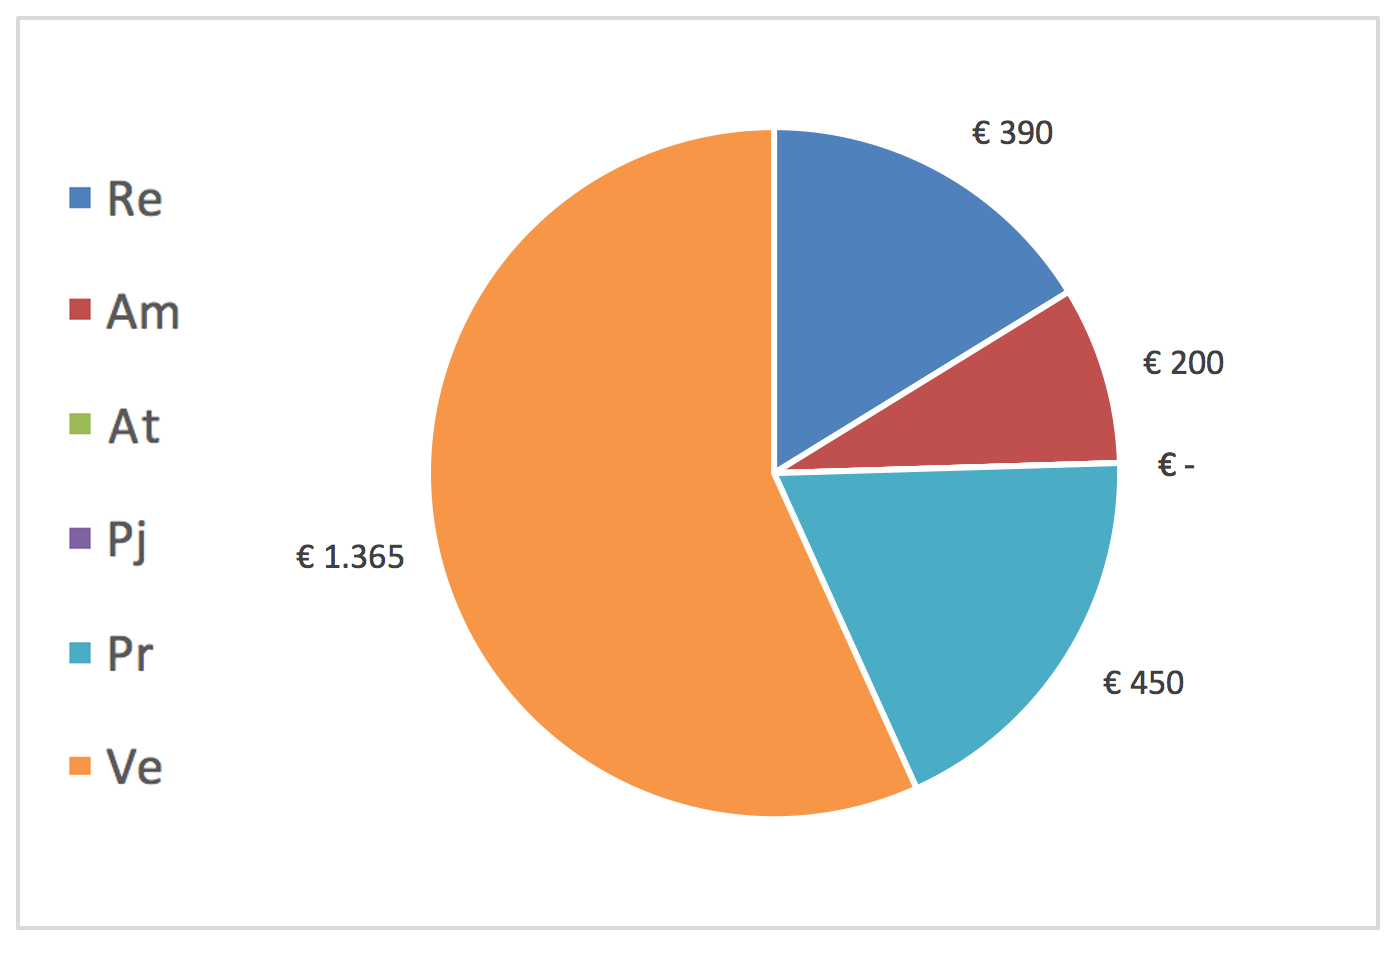
\includegraphics[scale=0.40]{img/s_Totale}
			\caption{Grafico del preventivo economico per ruolo - Totale complessivo}
			\label{fig:Totale complessivo economico}
			\end{figure}
%-----------------------------------------------------------------
		\newpage
		\subsection {Totale rendicontato}
				\subsubsection {Preventivo orario}
                Durante lo sviluppo del progetto, escludendo le ore non rendicontate, i membri del gruppo ricopriranno i vari ruoli secondo la seguente suddivisione:\\
%-----------------------------------------------------------------

							\begin{table}[H] \begin{center} \begin{tabular}{llllllll}
							\toprule
							\textbf{Nominativo}		&	\textbf{Re}	&	\textbf{Am}	&	\textbf{At}	&	\textbf{Pj}	&	\textbf{Pr}	&	\textbf{Ve}	&	\textbf{Tot}\\
							\midrule
							Brutesco	&	5	&	4	&	0	&	26	&	21	&	49	&	105	 \\
							Damo	&	5	&	0	&	0	&	39	&	22	&	39	&	105	 \\
							De Gaspari	&	10	&	10	&	0	&	18	&	25	&	42	&	105	 \\
							Gottardo	&	0	&	6	&	0	&	38	&	28	&	33	&	105	 \\
							Pasqualini	&	13	&	9	&	5	&	45	&	16	&	17	&	105	 \\
							Petenazzi	&	0	&	9	&	5	&	29	&	27	&	35	&	105	 \\
							Prete	&	10	&	0	&	0	&	16	&	32	&	47	&	105	 \\
							\midrule
							Tot in ore	&	43	&	38	&	10	&	211	&	171	&	262	&	735	 \\

							\bottomrule
							\end{tabular} \end{center} \caption{Prospetto orario -
							Totale rendicontato
							}\label{tab:h_TotaleRendicontato} \end{table}		\begin{figure}[H]  \centering  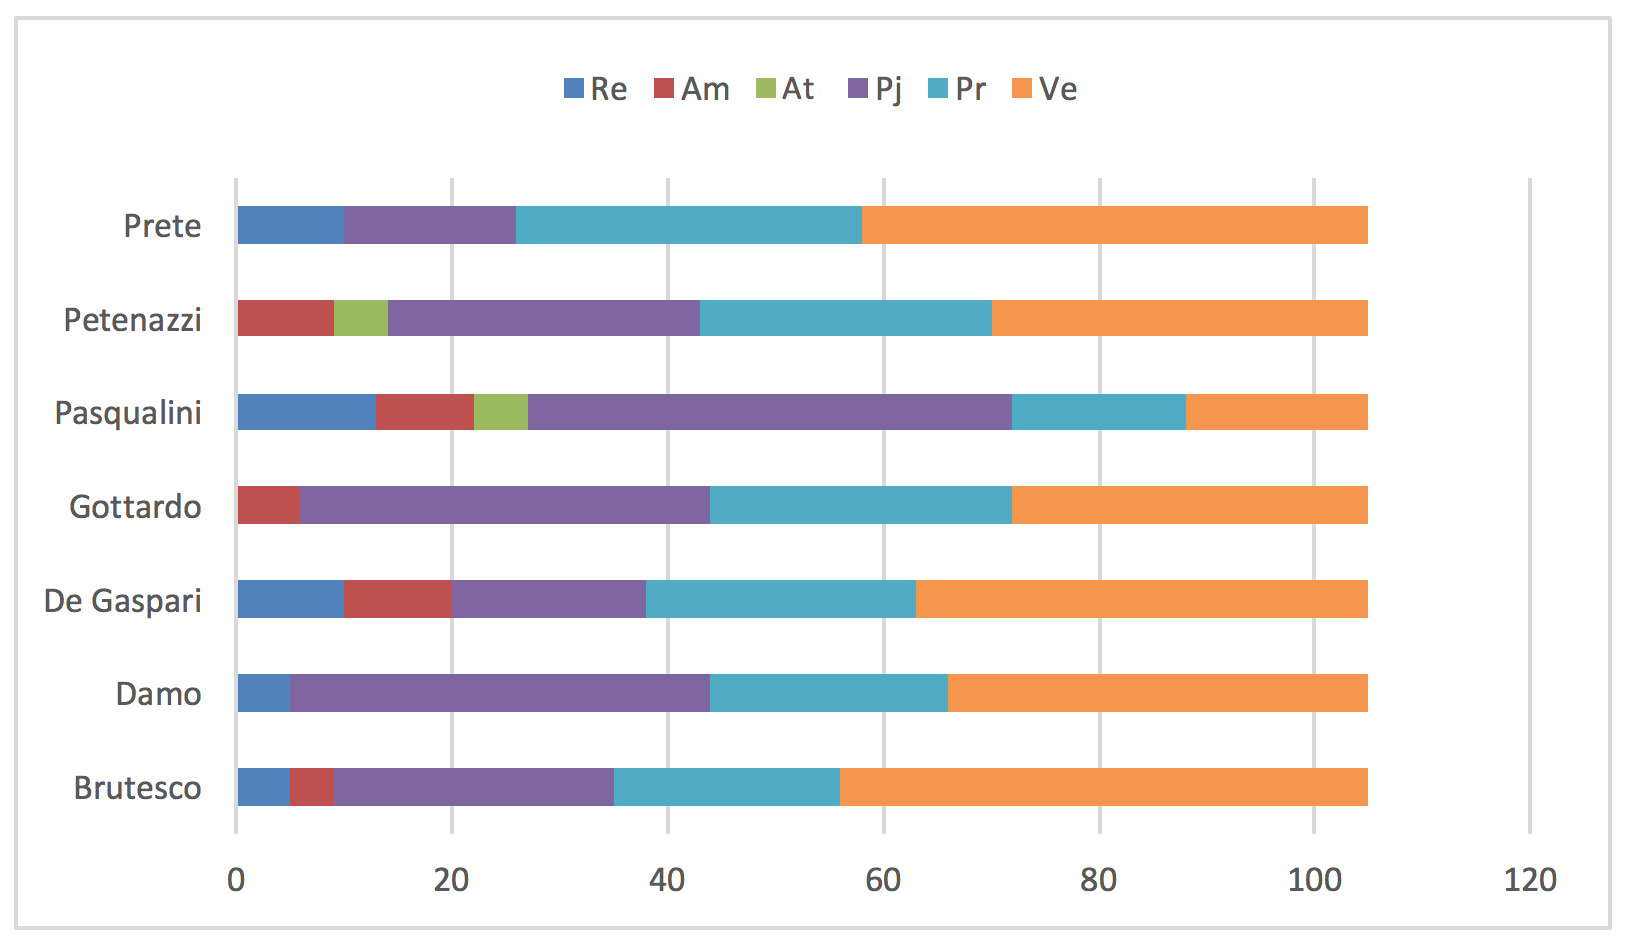
\includegraphics[scale=0.40]{img/h_TotaleRendicontato}
									\caption{Grafico del preventivo orario -								Totale rendicontato	}  \label{fig:h_TotaleRendicontato	} \end{figure}
%-----------------------------------------------------------------
							\begin{figure}[H]
							\centering
							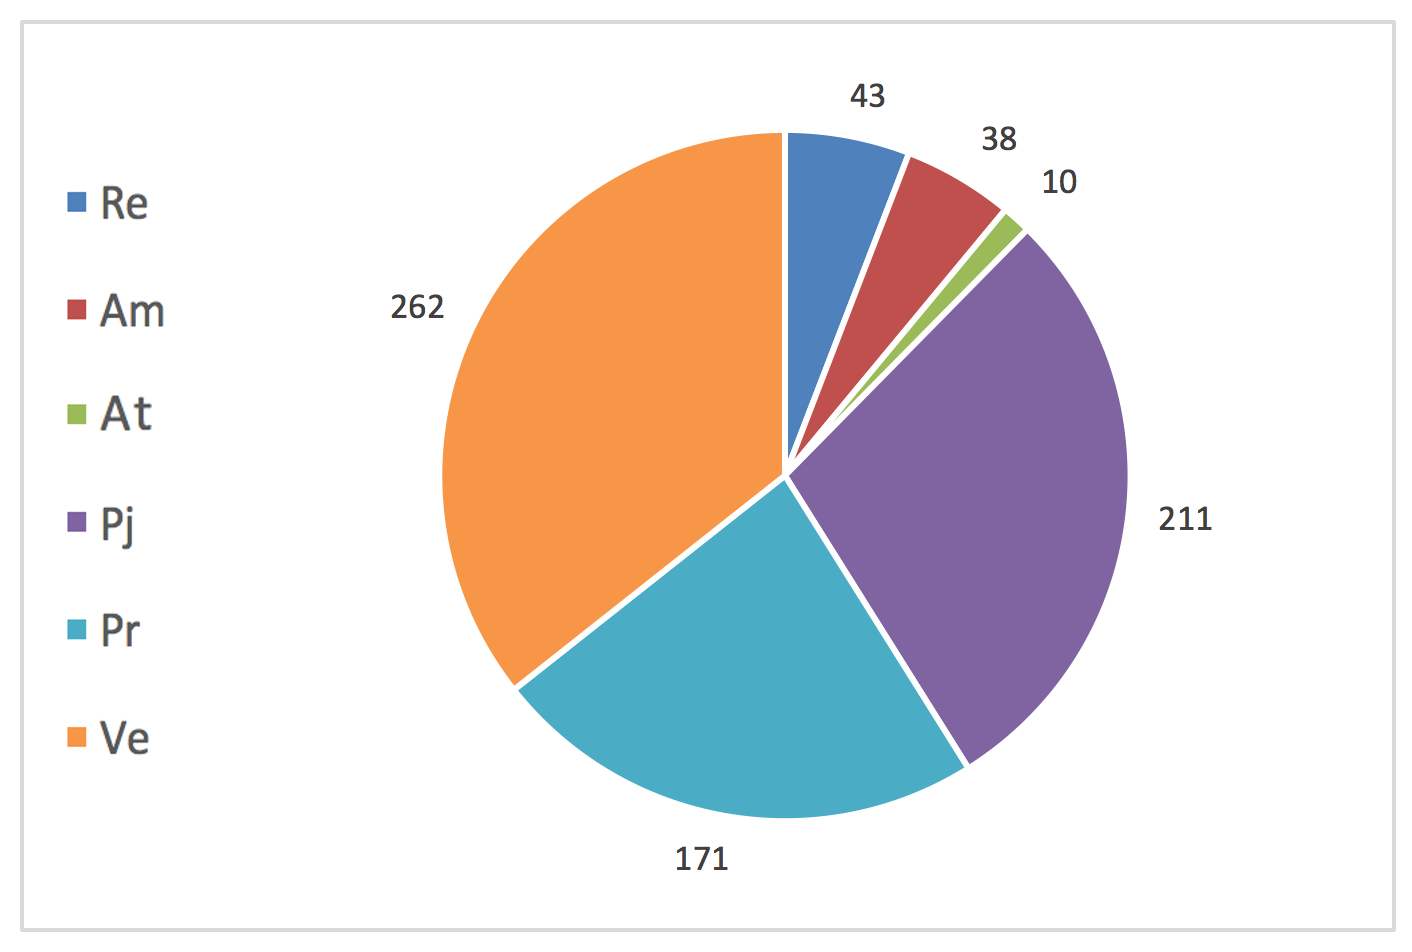
\includegraphics[scale=0.40]{img/h_r_TotaleRendicontato}
							\caption{Grafico del preventivo orario per ruolo - Totale rendicontato}
							\label{fig:Totale rendicontato orario"}
							\end{figure}
%-----------------------------------------------------------------
				\newpage
				\subsubsection {Preventivo economico}
%-----------------------------------------------------------------
							\begin{table}[H] \begin{center} \begin{tabular}{llllllll}
							\toprule
								&	\textbf{Re}	&	\textbf{Am}	&	\textbf{At}	&	\textbf{Pj}	&	\textbf{Pr}	&	\textbf{Ve}	&	\textbf{Tot}\\

							\midrule
							Tot in ore	&	43	&	38	&	10	&	211	&	171	&	262	&	735	 \\


							Tot in €	&	 €  1.290 	 & 	 €      760 	 & 	 €     250 	 & 	 €  4.642 	 & 	 € 2.565 	 & 	 €  3.930 	 & 	 €  13.437 	 \\
							\bottomrule
							\end{tabular} \end{center} \caption{Prospetto economico -
							Totale rendicontato
							}\label{tab:s_TotaleRendicontato} \end{table}
%-----------------------------------------------------------------
%-----------------------------------------------------------------

			\begin{figure}[H]
			\centering
			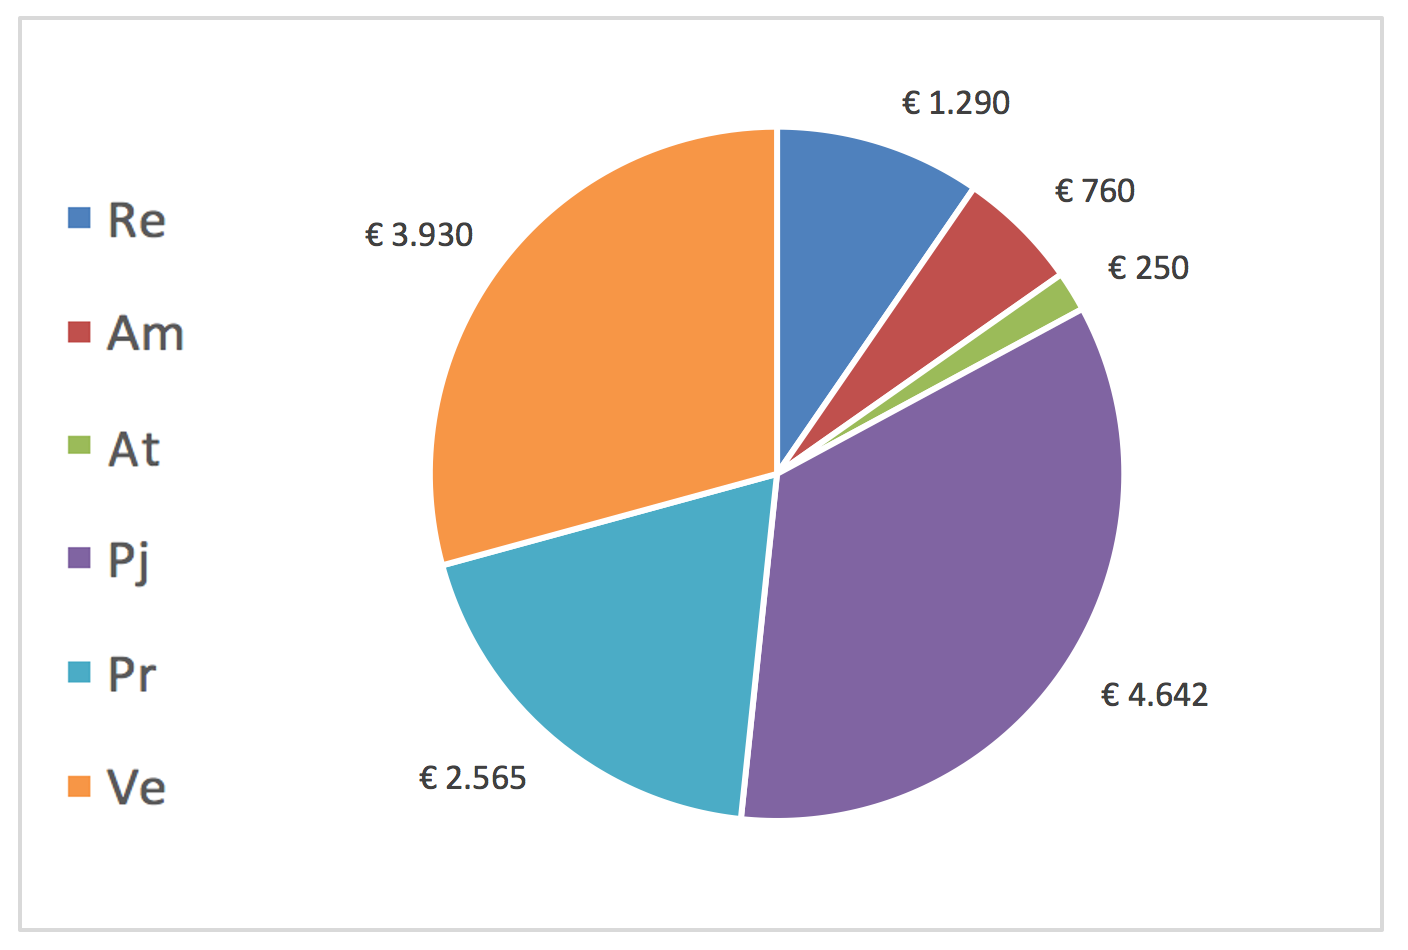
\includegraphics[scale=0.40]{img/s_TotaleRendicontato}
			\caption{Grafico del preventivo economico per ruolo - Totale rendicontato}
			\label{fig:Totale rendicontato economico"}
			\end{figure}
%-----------------------------------------------------------------
\subsection{Costo finale}
Il costo finale del progetto, indicato nella tabella \ref{tab:s_TotaleRendicontato}, viene arrotondato a € 13.430.

	%\section {Consuntivo}

\section {Consuntivo di periodo}
	\subsection {Introduzione}
	In questa sezione viene presentato il bilancio orario ed economico del progetto a consuntivo. Per ogni \glo{Periodo}{periodo} viene steso un consuntivo che mostra il quantitativo di ore rendicontate investite durante quel periodo e i totali (rendicontati, non rendicontati e complessivi) delle ore spese fino al termine del periodo preso in esame. Al termine del progetto verrà presentato un consuntivo finale.
	\\Il bilancio orario può essere:
	\begin{itemize}
	\item \textbf{positivo:} il preventivo orario ha superato il consuntivo orario;
	\item \textbf{negativo:} il consuntivo orario ha superato il preventivo orario;
	\item \textbf{in pari:} il preventivo orario conincide con il consuntivo orario.
	\end{itemize}
	Il bilancio economico può essere:
	\begin{itemize}
	\item \textbf{positivo:} il preventivo economico ha superato il consuntivo economico;
	\item \textbf{negativo:} il consuntivo economico ha superato il preventivo economico;
	\item \textbf{in pari:}  il preventivo economico conincide con il consuntivo economico.
	\end{itemize}
	
	\newpage
	\subsection {Dettaglio periodi}
		\subsubsection {Periodo: An - Analisi}
			\paragraph{Consuntivo di periodo orario}
			Si ricorda che le ore di questo periodo figurano come non rendicontate.
%---------------------------------------------------------------------
								\begin{table}[H] \begin{center} \begin{tabular}{llllllll}
								\toprule
								\textbf{Nominativo}	&	\textbf{Re}		&	\textbf{Am}		&	\textbf{At}		&	\textbf{Pj}		&	\textbf{Pr}		&	\textbf{Ve}		&	\textbf{Tot}		 \\
								\midrule																						 
								Brutesco	&	-		&	-		&	13	(+1)	&	-		&	-		&	12		&	25	(+1)\\
								Damo		&	-		&	9		&	16	(+1)	&	-		&	-		&	-		&	25	(+1)\\
								De Gaspari	&	-		&	-		&	13	(+1)	&	-		&	-		&	12		&	25	(+1)\\
								Gottardo	&	14		&	-		&	11	(+1)	&	-		&	-		&	-		&	25	(+1)\\
								Pasqualini	&	-		&	-		&	13	(+1)	&	-		&	-		&	12		&	25	(+1)\\
								Petenazzi	&	7		&	-		&	18	(+1)	&	-		&	-		&	-		&	25	(+1)\\
								Prete		&	-		&	10		&	15	(+1)	&	-		&	-		&	-		&	25	(+1)\\
								\midrule																					
								Tot in ore	&	21		&	19		&	99	(+7)	&	0		&	0		&	36		&	175	(+7)\\
								\bottomrule
								\end{tabular} \end{center} \caption{Prospetto orario a consuntivo per il periodo di analisi}\label{tab:oreAnalisiCons}
									\end{table}
%---------------------------------------------------------------------
			\paragraph{Consuntivo di periodo economico}
			La differenza tra le ore a consuntivo e preventivo di questo periodo non sono a carico del proponente e quindi saranno considerate solamente come ore di investimento non rendicontate.
%-----------------------------------------------------------------


								\begin{table}[H] \begin{center} \begin{tabular}{llllllll}
								\toprule
									&	\textbf{Re}	&	\textbf{Am}	&	\textbf{At}	&	\textbf{Pj}	&	\textbf{Pr}	&	\textbf{Ve}	&	\textbf{Tot}	 \\
								\midrule
								Tot in ore	&	21		&	19		&	99 (+7)	&	0		&	0		&	36		&	175	(+7)\\
								Tot in €	&	 € 630 		&	 € 380 		&	 € 2.475 		&	 € -   		&	 € -   		&	 € 540 		&	 € 4.025 	\\
								\bottomrule
								\end{tabular} \end{center} \caption{Prospetto economico - Periodo:
								An
								}\label{tab:sAnCons} \end{table}

%-----------------------------------------------------------------
			\paragraph{Conclusioni}
			Il lavoro degli \analisti{} ha richiesto più tempo di quello preventivato in quanto lo studio del dominio si è dimostrato più difficile di quanto previsto. Come si vede dalla tabella \ref{tab:oreAnalisiCons} il bilancio orario risulta negativo in quanto eccede di 7 ore rispetto a quanto pianificato.
			Come si vede dalla tabella \ref{tab:sAnCons} il bilancio economico è negativo per un importo pari a -175€.
			Queste variazioni rispetto al preventivo non avranno impatto sul costo finale in quanto le ore aggiuntive sono considerate di investimento.

%---------------------------------------------------------------------------------
	\newpage
	\subsubsection{Pl - Progettazione logica}
	\paragraph{Consuntivo di periodo orario}
%-----------------------------------------------------------------------------------
								\begin{table}[h] \begin{center} \begin{tabular}{llllllll}																						
								\toprule																						
									&	Re		&	Am		&	An		&	Pj		&	Pr		&	Ve		&	Tot	 \\ 	
								\midrule																		
								Brutesco	&	5		&	-		&	-		&	21		&	-		&	-		&	26	\\
								Damo		&	5		&	-		&	-		&	30		&	-		&	-		&	35	\\
								De Gaspari	&	-		&	-		&	-		&	6	(-4)	&	-		&	20	(+4)	&	26	\\
								Gottardo	&			&	-		&	-		&	10		&	-		&	16		&	26	\\
								Pasqualini	&	-		&	5		&	5		&	16		&	-		&	-		&	26	\\
								Petenazzi	&	-		&	4		&	5		&	17		&	-		&	-		&	26	\\
								Prete	&	-		&	-		&	-		&	14	(+4)	&	-		&	12	(-4)	&	26	\\
								\midrule																					
								Tot in ore	&	10		&	9		&	10		&	114(+0)		&	0		&	48(+0)		&	191	\\
								
								\bottomrule
								\end{tabular} \end{center} \caption{Prospetto a consuntivo orario per il periodo di																						
									Progettazione logica																						
									}\label{tab:orePl} \end{table}	
%-----------------------------------------------------------------------------------
	\paragraph{Consuntivo di periodo economico}
%-----------------------------------------------------------------------------------
								\begin{table}[H] \begin{center} \begin{tabular}{llllllll}																						
							\toprule	
								&	Re		&	Am		&	An		&	Pj		&	Pr		&	Ve		&	Tot	 \\ 	
							\midrule																		
							Tot in ore	&	10		&	9		&	10		&	114(+0)		&	0		&	48(+0)		&	191	\\
							Tot in €	&	 € 300 		 & 	 € 180 		 & 	 € 250 		 & 	 € 2.508 		 & 	 € -   		 & 	 € 720 		 & 	 € 3.958 	\\
							\bottomrule																						
							\end{tabular} \end{center} \caption{Prospetto a consuntivo economico per il periodo di																						
							Progettazione logica																						
							}\label{tab:sPl} \end{table}
	
	%----------------------------------------------------------------------------	
				\paragraph{Conclusioni}
				E’ stato necessario un ricalibro delle ore a causa di problemi personali di un membro, come indicato
				dall’analisi dei rischi. Nonostante ciò, il consuntivo orario presenta gli stessi totali esposti nel preventivo orario di questo periodo.
%---------------------------------------------------------------------------------
\newpage
\subsubsection{PCV - Progettazione Codifica Validazione}
\paragraph{Consuntivo di periodo orario}
%-----------------------------------------------------------------------------------
							\begin{table}[H] \begin{center} \begin{tabular}{llllllll}
										\toprule
										\textbf{Nominativo}	&	\textbf{Re}	&	\textbf{Am}	&	\textbf{At}	&	\textbf{Pj}	&	\textbf{Pr}	&	\textbf{Ve}	&	\textbf{Tot}\\
										\midrule
										Brutesco	&	-		&	4		&	-		&	5		&	14	(-1)&	29	&	52	\\
										Damo		&	-		&	-		&	1	(+1)&	9		&	20	(-2)&	39	&	69	\\
										De Gaspari	&	10		&	-		&	-		&	8		&	24	(-1)&	13	&	55	\\
										Gottardo	&	-		&	6		&	-		&	28		&	21	(-1)&	-	&	55	\\
										Pasqualini	&	-		&	4		&	-		&	29		&	15	(-1)&	7	&	55	\\
										Petenazzi	&	-		&	5		&	-		&	12		&	19	(-1)&	19	&	55	\\
										Prete		&	10		&	-		&	-		&	6		&	20	(-1)&	16	&	52	\\
										\midrule																				
										Tot in ore	&	20		&	19		&	1	(+1)&	97		&	133	(-8)&	123	&	393	(-7)\\
																				
										\bottomrule
									\end{tabular} \end{center} \caption{Consuntivo di periodo orario - Periodo:
									PCV
								} \end{table}
%-----------------------------------------------------------------------------------
\paragraph{Consuntivo di periodo economico}
%-----------------------------------------------------------------------------------
\begin{table}[H] \begin{center} \begin{tabular}{llllllll}																						
			\toprule	
			&	Re		&	Am		&	An		&	Pj		&	Pr		&	Ve		&	Tot	 \\ 	
			\midrule																		
			Tot in ore	&	20		&	19		&	1	(+1)&	97		&	133	(-8)&	123	&	393	(-7)\\
			Tot in €	&	 € 600 		 & 	 € 380 		 & 	 € 25 		 & 	 € 2.134 		 & 	 € 1.995 		 & 	 € 1.845 		 & 	 € 6.979 	\\
			\bottomrule																						
		\end{tabular} \end{center} \caption{Prospetto a consuntivo economico per il periodo PCV																					
	}\label{tab:s_PCV_c} \end{table}

%----------------------------------------------------------------------------	

				
	\paragraph{Conclusioni}
	A livello di pianificazione, i codificatori hanno impiegato più tempo di quanto previsto, anche a causa di un rischio non preventivato che si è verificato: non sono state seguite le norme di codifica stabilite. La codifica è stata, specialmente nei momenti iniziali poco organizzata e alquanto indisciplinata. Il \responsabile{} ha cercato di arginare il fenomeno richiamando gli amministratori in modo che stabilissero un maggior rigore specialmente per quanto riguarda :
	\begin{itemize}
		\item il controllo di configurazione;
		\item l'integrazione degli strumenti e delle tecnologie.
	\end{itemize}
	Le conseguenze principali sono:
	\begin{itemize}
		\item gli incrementi 5, 6, 7, 8 pianificati (legati a requisiti facoltativi) non sono stati svolti;
		\item negli incrementi 1, 2, 3, 4, si è:
				\begin{itemize}
					\item progettato a basso livello l'incremento;
					\item parzialmente codificato l'incremento;
					\item parzialmente effettuati i test di unita dell'incremento.
				\end{itemize}
			non effettuando alcuna validazione del prodotto, e portando di fatto a uno sviluppo di carattere sequenziale.
	\end{itemize}
	Il sorgere di alcuni problemi col proponente come indicato dall'analisi dei rischi, ha portato alla formazione di un'ora di analisi, necessaria per la modifica dell' \adr{} e a una diminuzione delle ore di codifica, anche grazie al fatto che non si sono svolti gli incrementi opzionali.
	Il consuntivo orario ed economico presenta quindi delle variazioni rispetto a quanto era stato preventivato nelle tabelle \ref{tab:h_PCV} e \ref{tab:s_PCV}. In particolare sono state impiegate 7 ore in meno diminuendo la spesa di 95€.
	Per cercare di risolvere questi problemi, è stato steso un adeguato preventivo a finire in  \ref{preventivo_a_finire}.
	\newpage
	\subsection{Totale non rendicontato}
		\subsubsection{Consuntivo di periodo orario}
%-----------------------------------------------------------------
						\begin{table}[h] \begin{center} \begin{tabular}{llllllll}																						
						\toprule
									&	Re		&	Am		&	An		&	Pj		&	Pr		&	Ve		&	Tot	 \\ 	
						\midrule																					
						Brutesco	&	2		&	3		&	14		&	2		&	2		&	14		&	37		\\
						Damo	&	2		&	12		&	17		&	2		&	2		&	2		&	37		\\
						De Gaspari	&	2		&	0		&	14		&	2		&	2		&	14		&	34		\\
						Gottardo	&	16		&	3		&	12		&	2		&	2		&	2		&	37		\\
						Pasqualini	&	0		&	3		&	14		&	2		&	2		&	14		&	35		\\
						Petenazzi	&	9		&	3		&	19		&	2		&	2		&	2		&	37		\\
						Prete	&	2		&	13		&	16		&	2	&	2		&	2		&	37		\\
						\midrule																Tot in ore	&	33		&	37		&	106		&	14		&	14		&	50		&	254		\\	
						\bottomrule																						
						\end{tabular} \end{center} \caption{Prospetto orario a consuntivo totale non rendicontato fino alla fine del periodo PCV																						
						}\label{tab:oreNonRend} \end{table}							
%-----------------------------------------------------------------
		\subsubsection{Consuntivo di periodo economico}
%-----------------------------------------------------------------
						\begin{table}[H] \begin{center} \begin{tabular}{llllllll}
						\toprule
							&	\textbf{Re}	&	\textbf{Am}	&	\textbf{At}	&	\textbf{Pj}	&	\textbf{Pr}	&	\textbf{Ve}	&	\textbf{Tot}\\
			
						\midrule
						Tot in ore	&	33		&	37		&	106		&	14		&	14		&	50		&	254		\\
						Tot in €	&	 € 990 		 & 	 € 740 		 & 	 € 2.650 		 & 	 € 308 		 & 	 € 210 		 & 	 € 750 		 & 	 € 5.648 		\\
						\bottomrule
						\end{tabular} \end{center} \caption{Prospetto economico a consuntivo totale non rendicontato fino alla fine del periodo PCV		
						}\label{tab:s_TotaleNonRendicontato} \end{table}
%-----------------------------------------------------------------
	
	\newpage
	\subsection{Totale complessivo}
		\subsubsection{Consuntivo di periodo orario}

%-----------------------------------------------------------------------------------------																					
						\begin{table}[h] \begin{center} \begin{tabular}{llllllll}																					
						\toprule																					
							&	Re		&	Am		&	An		&	Pj		&	Pr		&	Ve		&	Tot	\\
						\midrule																					
						Brutesco	&	7		&	7		&	14		&	28		&	16		&	43		&	115	\\
						Damo	&	7		&	12		&	18		&	41		&	22		&	41		&	141	\\
						De Gaspari	&	12		&	0		&	14		&	16		&	26		&	47		&	115	\\
						Gottardo	&	16		&	9		&	12		&	40		&	23		&	18		&	118	\\
						Pasqualini	&	0		&	12		&	19		&	47		&	17		&	21		&	116	\\
						Petenazzi	&	9		&	12		&	24		&	31		&	21		&	21		&	118	\\
						Prete	&	12		&	13		&	16		&	22		&	22		&	30		&	115	\\
						\midrule																					
						Tot in ore	&	63		&	65		&	117		&	225		&	147		&	221		&	838	\\
						\bottomrule																					
						\end{tabular} \end{center} \caption{Prospetto orario a consuntivo totale complessivo fino alla fine del periodo PCV															
						} \end{table}
%-----------------------------------------------------------------------------------------																					
		\subsubsection{Consuntivo di periodo economico}
%-----------------------------------------------------------------
						\begin{table}[H] \begin{center} \begin{tabular}{llllllll}
						\toprule
							&	\textbf{Re}	&	\textbf{Am}	&	\textbf{At}	&	\textbf{Pj}	&	\textbf{Pr}	&	\textbf{Ve}	&	\textbf{Tot}\\
						\midrule																					
						Tot in ore	&	63		&	65		&	117		&	225		&	147		&	221		&	838	\\
						Tot in €	&	 € 1.890 		 & 	 € 1.300 		 & 	 € 2.925 		 & 	 € 4.950 		 & 	 € 2.205 		 & 	 € 3.315 		 & 	 € 16.585 	\\
						\bottomrule			
						\end{tabular} \end{center} \caption{Prospetto economico a consuntivo totale complessivo fino alla fine del periodo PCV			
						}\label{tab:s_TotaleNonRendicontato} \end{table}
%-----------------------------------------------------------------
	
	\newpage
	\subsection{Totale rendicontato}
		\subsubsection{Consuntivo di periodo orario}
		
		%-----------------------------------------------------------------------------------------																					
		\begin{table}[h] \begin{center} \begin{tabular}{llllllll}																					
					\toprule																					
					&	Re		&	Am		&	An		&	Pj		&	Pr		&	Ve		&	Tot	\\
					\midrule																					
					Brutesco	&	5		&	4		&	0		&	26		&	14		&	29		&	78	\\
					Damo		&	5		&	0		&	1		&	39		&	20		&	39		&	104	\\
					De Gaspari	&	10		&	0		&	0		&	14		&	24		&	33		&	81	\\
					Gottardo	&	0		&	6		&	0		&	38		&	21		&	16		&	81	\\
					Pasqualini	&	0		&	9		&	5		&	45		&	15		&	7		&	81	\\
					Petenazzi	&	0		&	9		&	5		&	29		&	19		&	19		&	81	\\
					Prete		&	10		&	0		&	0		&	20		&	20		&	28		&	78	\\
					\midrule																					
					Tot in ore	&	30		&	28		&	11		&	211		&	133		&	171		&	584	\\
					\bottomrule																					
				\end{tabular} \end{center} \caption{Prospetto orario a consuntivo totale rendicontato fino alla fine del periodo PCV															
			} \end{table}
			%-----------------------------------------------------------------------------------------																					
			\subsubsection{Consuntivo di periodo economico}
			%-----------------------------------------------------------------
			\begin{table}[H] \begin{center} \begin{tabular}{llllllll}
						\toprule
						&	\textbf{Re}	&	\textbf{Am}	&	\textbf{At}	&	\textbf{Pj}	&	\textbf{Pr}	&	\textbf{Ve}	&	\textbf{Tot}\\
						\midrule																					
						Tot in ore	&	30		&	28		&	11		&	211		&	133		&	171		&	584	\\
						Tot in €	&	 € 900 		 & 	 € 560 		 & 	 € 275 		 & 	 € 4.642 		 & 	 € 1.995 		 & 	 € 2.565 		 & 	 € 10.937 	\\
						\bottomrule			
					\end{tabular} \end{center} \caption{Prospetto economico a consuntivo totale rendicontato fino alla fine il periodo PCV	
				}\label{tab:s_TotaleNonRendicontato} \end{table}
			%-----------------------------------------------------------------

.
	\subsection{Considerazioni finali sul consuntivo di periodo}
	\label{consid_cons_pl}
	Il totale rendicontato a consuntivo (e di conseguenza anche quello complessivo) presenta delle variazioni rispetto a quanto preventivato; in particolare il bilancio orario si chiude in positivo di 7 ore, mentre quello economico si chiude in positivo di 95€. Grazie a quanto emerso nell'analisi dei rischi e nel consuntivo di fine periodo è stato steso un adeguato preventivo a finire in  \ref{preventivo_a_finire}.
	%\section {Preventivo a finire}
\section {Preventivo a finire}
	\subsection {Introduzione}
	In questa sezione viene rivisto il preventivo sulla base delle eventuali variazioni esposte nel consuntivo di fine periodo.
	\subsection {Dettaglio fasi}
		\subsubsection {Fase: Pl - Progettazione logica}
			\paragraph{Preventivo orario}

							\begin{table}[H] \begin{center} \begin{tabular}{llllllll}
							\toprule
							\textbf{Nominativo}	&	\textbf{Re}	&	\textbf{Am}	&	\textbf{At}	&	\textbf{Pj}	&	\textbf{Pr}	&	\textbf{Ve}	&	\textbf{Tot}	 \\
							\midrule
							Brutesco	&	5	&	-	&	-	&	21	&	-	&	-	&	26	 \\
							Damo	&	5	&	-	&	-	&	30	&	-	&	-	&	35	 \\
							De Gaspari	&	-	&	-	&	-	&	10	&	-	&	16	&	26	 \\
							Gottardo	&	-	&	-	&	-	&	10	&	-	&	16	&	26	 \\
							Pasqualini	&	-	&	5	&	5	&	16	&	-	&	-	&	26	 \\
							Petenazzi	&	-	&	4	&	5	&	17	&	-	&	-	&	26	 \\
							Prete	&	-	&	-	&	-	&	10	&	-	&	16	&	26	 \\
							\midrule
							Tot in ore	&	10	&	9	&	10	&	114	&	0	&	48	&	191	 \\

							\bottomrule
							\end{tabular} \end{center} \caption{Prospetto orario preventivo a finire - Fase:
							Pl
							} \end{table}

			\paragraph{Preventivo economico}
							\begin{table}[H] \begin{center} \begin{tabular}{llllllll}
							\toprule
							\textbf{Nominativo}	&	\textbf{Re}	&	\textbf{Am}	&	\textbf{At}	&	\textbf{Pj}	&	\textbf{Pr}	&	\textbf{Ve}	&	\textbf{Tot}	 \\

							\midrule
							Tot in ore	&	10	&	9	&	10	&	114	&	0	&	48	&	191	 \\


							Tot in €	&	 €     300 	 & 	 €      180 	 & 	 €     250 	 & 	 €  2.508 	 & 	 €        -   	 & 	 €     720 	 & 	 €     3.958 	 \\
							\bottomrule
							\end{tabular} \end{center} \caption{Prospetto economico preventivo a finire - Fase:
							Pl
							} \end{table}


			\paragraph{Conclusioni} Il preventivo a finire di questa \glo{Fase}{fase} è rimasto invariato rispetto al prospetto presentato nelle tabelle \ref{tab:h_Pl} e \ref{tab:s_Pl}.
		\newpage
		\subsubsection {Fase: PdROb - Progettazione di dettaglio e codifica Requisiti Obbligatori}
			\paragraph{Preventivo orario}
											\begin{table}[H] \begin{center} \begin{tabular}{llllllll}
											\toprule
											\textbf{Nominativo}	&	\textbf{Re}	&	\textbf{Am}	&	\textbf{At}	&	\textbf{Pj}	&	\textbf{Pr}	&	\textbf{Ve}	&	\textbf{Tot}	 \\
											\midrule
											Brutesco	&	-	&	-	&	-	&	5	&	9	&	16	&	30	 \\
											Damo	&	-	&	-	&	-	&	5	&	14	&	19	&	38	 \\
											De Gaspari	&	10	&	-	&	-	&	8	&	12	&	-	&	30	 \\
											Gottardo	&	-	&	6	&	-	&	12	&	12	&	-	&	30	 \\
											Pasqualini	&	-	&	4	&	-	&	13	&	13	&	-	&	30	 \\
											Petenazzi	&	-	&	-	&	-	&	8	&	6	&	16	&	30	 \\
											Prete	&	-	&	-	&	-	&	6	&	8	&	16	&	30	 \\
											\midrule
											Tot in ore	&	10	&	10	&	0	&	57	&	74	&	67	&	218	 \\

											\bottomrule
											\end{tabular} \end{center} \caption{Prospetto orario preventivo a finire - Fase:
											PdROb
											} \end{table}

				\paragraph{Preventivo economico}
											\begin{table}[H] \begin{center} \begin{tabular}{llllllll}
											\toprule
												&	\textbf{Re}	&	\textbf{Am}	&	\textbf{At}	&	\textbf{Pj}	&	\textbf{Pr}	&	\textbf{Ve}	&	\textbf{Tot}	 \\

											\midrule
											Tot in ore	&	10	&	10	&	0	&	57	&	74	&	67	&	218	 \\


											Tot in €	&	 €           300 	 & 	 €        200 	 & 	 €               -   	 & 	 €    1.254 	 & 	 €        1.110 	 & 	 €    1.005 	 & 	 €              3.869 	 \\
											\bottomrule
											\end{tabular} \end{center} \caption{Prospetto economico preventivo a finire - Fase:
											PdROb
											} \end{table}
			\paragraph{Preventivo} Il preventivo a finire di questa \glo{Fase}{fase} è rimasto invariato rispetto al prospetto presentato nelle tabelle \ref{tab:h_PdROb} e \ref{tab:s_PdROb}.
		\newpage
		\subsubsection {Fase: PdRD - Progettazione di dettaglio e codifica Requisiti Desiderabili}
			\paragraph{Preventivo orario}
				\begin{table}[H] \begin{center} \begin{tabular}{llllllll}
										\toprule
										\textbf{Nominativo}	&	\textbf{Re}	&	\textbf{Am}	&	\textbf{At}	&	\textbf{Pj}	&	\textbf{Pr}	&	\textbf{Ve}	&	\textbf{Tot}	 \\
										\midrule
										Brutesco	&	-	&	-	&	-	&	-	&	6	&	13	&	19	 \\
										Damo		&	-	&	-	&	-	&	-	&	8	&	17	&	25	 \\
										De Gaspari	&	-	&	-	&	-	&	-	&	6	&	13	&	19	 \\
										Gottardo	&	-	&	-	&	-	&	16	&	3	&	-	&	19	 \\
										Pasqualini	&	-	&	-	&	-	&	16	&	3	&	-	&	19	 \\
										Petenazzi	&	-	&	5	&	-	&	-	&	14	&	-	&	19	 \\
										Prete		&	6	&	-	&	-	&	-	&	13	&	-	&	19	 \\
										\midrule
										Tot in ore	&	6	&	5	&	0	&	32	&	53	&	43	&	139	 \\


										\bottomrule
										\end{tabular} \end{center} \caption{Prospetto orario preventivo a finire - Fase:
										PdRD
										} \end{table}

			\paragraph{Preventivo economico}
										\begin{table}[H] \begin{center} \begin{tabular}{llllllll}
										\toprule
											&	\textbf{Re}	&	\textbf{Am}	&	\textbf{At}	&	\textbf{Pj}	&	\textbf{Pr}	&	\textbf{Ve}	&	\textbf{Tot}	 \\

										\midrule
										Tot in ore	&	6	&	5	&	0	&	32	&	53	&	43	&	139	 \\


										Tot in €	&	 €     180 	 & 	 €      100 	 & 	 €         -   	 & 	 €     704 	 & 	 €    795 	 & 	 €     645 	 & 	 €     2.424 	 \\
										\bottomrule
										\end{tabular} \end{center} \caption{Prospetto economico preventivo a finire - Fase:
										PdRD
										} \end{table}

			\paragraph{Preventivo} Il preventivo a finire di questa \glo{Fase}{fase} è rimasto invariato rispetto al prospetto presentato nelle tabelle \ref{tab:h_PdRD} e \ref{tab:s_PdRD}.
		\newpage
		\subsubsection {Fase: PdROp - Progettazione di dettaglio e codifica Requisiti Opzionali}
			\paragraph{Preventivo orario}
								\begin{table}[H] \begin{center} \begin{tabular}{llllllll}
										\toprule
										\textbf{Nominativo}	&	\textbf{Re}	&	\textbf{Am}	&	\textbf{At}	&	\textbf{Pj}	&	\textbf{Pr}	&	\textbf{Ve}	&	\textbf{Tot}	 \\
										\midrule
										Brutesco	&	-	&	4	&	-	&	-	&	-	&	-	&	4	 \\
										Damo	&	-	&	-	&	-	&	4	&	-	&	3	&	7	 \\
										De Gaspari	&	-	&	-	&	-	&	-	&	7	&	-	&	7	 \\
										Gottardo	&	-	&	-	&	-	&	-	&	7	&	-	&	7	 \\
										Pasqualini	&	-	&	-	&	-	&	-	&	-	&	7	&	7	 \\
										Petenazzi	&	-	&	-	&	-	&	4	&	-	&	3	&	7	 \\
										Prete	&	4	&	-	&	-	&	-	&	-	&	-	&	4	 \\
										\midrule
										Tot in ore	&	4	&	4	&	0	&	8	&	14	&	13	&	43	 \\



										\bottomrule
										\end{tabular} \end{center} \caption{Prospetto orario preventivo a finire - Fase:
										PdROp
										} \end{table}

			\paragraph{Preventivo economico}
										\begin{table}[H] \begin{center} \begin{tabular}{llllllll}
										\toprule
											&	\textbf{Re}	&	\textbf{Am}	&	\textbf{At}	&	\textbf{Pj}	&	\textbf{Pr}	&	\textbf{Ve}	&	\textbf{Tot}	 \\

										\midrule
										Tot in ore	&	4	&	4	&	0	&	8	&	14	&	13	&	43	 \\


										Tot in €	&	 €           120 	 & 	 €          80 	 & 	 €               -   	 & 	 €        176 	 & 	 €            210 	 & 	 €        195 	 & 	 €                 781 	 \\
										\bottomrule
										\end{tabular} \end{center} \caption{Prospetto economico preventivo a finire - Fase:
										PdROp
										} \end{table}
			\paragraph{Preventivo} Il preventivo a finire di questa \glo{Fase}{fase} è rimasto invariato rispetto al prospetto presentato nelle tabelle \ref{tab:h_PdROp} e \ref{tab:s_PdROp}.
		\newpage
		\subsubsection {Fase: Va - Validazione}
			\paragraph{Preventivo orario}
			\begin{table}[H] \begin{center} \begin{tabular}{llllllll}
										\toprule
										\textbf{Nominativo}	&	\textbf{Re}	&	\textbf{Am}	&	\textbf{At}	&	\textbf{Pj}	&	\textbf{Pr}	&	\textbf{Ve}	&	\textbf{Tot}	 \\
										\midrule
										Brutesco	&	-	&	-	&	-	&	-	&	6	&	20	&	26	 \\
										Damo	&	-	&	-	&	-	&	-	&	-	&	-	&	0	 \\
										De Gaspari	&	-	&	10	&	-	&	-	&	-	&	13	&	23	 \\
										Gottardo	&	-	&	-	&	-	&	-	&	6	&	17	&	23	 \\
										Pasqualini	&	13	&	-	&	-	&	-	&	-	&	10	&	23	 \\
										Petenazzi	&	-	&	-	&	-	&	-	&	7	&	16	&	23	 \\
										Prete	&	-	&	-	&	-	&	-	&	11	&	15	&	26	 \\
										\midrule
										Tot in ore	&	13	&	10	&	0	&	0	&	30	&	91	&	144	 \\


										\bottomrule
										\end{tabular} \end{center} \caption{Prospetto orario preventivo a finire - Fase:
										Va
										}\end{table}
			\paragraph{Preventivo economico}
				\begin{table}[H] \begin{center} \begin{tabular}{llllllll}
										\toprule
											&	\textbf{Re}	&	\textbf{Am}	&	\textbf{At}	&	\textbf{Pj}	&	\textbf{Pr}	&	\textbf{Ve}	&	\textbf{Tot}	 \\

										\midrule
										Tot in ore	&	13	&	10	&	0	&	0	&	30	&	91	&	144	 \\


										Tot in €	&	 €     390 	 & 	 €      200 	 & 	 €         -   	 & 	 €         -   	 & 	 €    450 	 & 	 €  1.365 	 & 	 €     2.405 	 \\
										\bottomrule
										\end{tabular} \end{center} \caption{Prospetto economico preventivo a finire - Fase:
										Va
										}\end{table}
			\paragraph{Conclusioni} Il preventivo a finire di questa \glo{Fase}{fase} è rimasto invariato rispetto al prospetto presentato nelle tabelle \ref{tab:h_Va} e \ref{tab:s_Va}.
	\newpage
	\subsection{Totale non rendicontato}
		\subsubsection{Preventivo orario}


			\begin{table}[H] \begin{center} \begin{tabular}{llllllll}
			\toprule
			\textbf{Nominativo}	&	\textbf{Re}	&	\textbf{Am}	&	\textbf{At}	&	\textbf{Pj}	&	\textbf{Pr}	&	\textbf{Ve}	&	\textbf{Tot}	 \\
			\midrule
			Brutesco	&	2	&	3	&	15	&	2	&	2	&	14	&	38	 \\
			Damo	&	2	&	12	&	18	&	2	&	2	&	2	&	38	 \\
			De Gaspari	&	2	&	3	&	15	&	2	&	2	&	14	&	38	 \\
			Gottardo	&	16	&	3	&	13	&	2	&	2	&	2	&	38	 \\
			Pasqualini	&	2	&	3	&	15	&	2	&	2	&	14	&	38	 \\
			Petenazzi	&	9	&	3	&	20	&	2	&	2	&	2	&	38	 \\
			Prete	&	2	&	13	&	17	&	2	&	2	&	2	&	38	 \\
			\midrule
			Tot in ore	&	35	&	40	&	113	&	14	&	14	&	50	&	266	 \\


			\bottomrule
			\end{tabular} \end{center} \caption{Prospetto orario preventivo a finire -
			Totale non rendicontato
			} \end{table}

		\subsubsection{Preventivo economico}

			\begin{table}[H] \begin{center} \begin{tabular}{llllllll}
			\toprule
				&	\textbf{Re}	&	\textbf{Am}	&	\textbf{At}	&	\textbf{Pj}	&	\textbf{Pr}	&	\textbf{Ve}	&	\textbf{Tot}	 \\
			\midrule
			Tot in ore	&	35	&	40	&	113	&	14	&	14	&	50	&	266	 \\
			Tot. in €	&	 €  1.050 	 & 	 €  800	 & 	 €  2.825	 & 	 €  308 	 & 	 €  210 & 	 €  750	 & 	 €        5.943 	 \\			\bottomrule
			\end{tabular} \end{center}
			\caption{Prospetto orario preventivo a finire - Totale non rendicontato
			} \end{table}

	\subsubsection{Conclusioni} Il preventivo a finire di questa \glo{Fase}{fase} presenta delle variazioni rispetto al prospetto presentato nelle tabelle \ref{tab:h_TotaleNonRendicontato} e \ref{tab:s_TotaleNonRendicontato}.

	\newpage
	\subsection{Totale complessivo}
		\subsubsection{Preventivo orario}

			\begin{table}[H] \begin{center} \begin{tabular}{llllllll}
			\toprule
			\textbf{Nominativo}	&	\textbf{Re}	&	\textbf{Am}	&	\textbf{At}	&	\textbf{Pj}	&	\textbf{Pr}	&	\textbf{Ve}	&	\textbf{Tot}	 \\
			\midrule
			Brutesco	&	7	&	7	&	15	&	28	&	23	&	63	&	143	 \\
			Damo	&	7	&	12	&	18	&	41	&	24	&	41	&	143	 \\
			De Gaspari	&	12	&	13	&	15	&	20	&	27	&	56	&	143	 \\
			Gottardo	&	16	&	9	&	13	&	40	&	30	&	35	&	143	 \\
			Pasqualini	&	15	&	12	&	20	&	47	&	18	&	31	&	143	 \\
			Petenazzi	&	9	&	12	&	25	&	31	&	29	&	37	&	143	 \\
			Prete	&	12	&	13	&	17	&	18	&	34	&	49	&	143	 \\
			\midrule
			Tot in ore	&	78	&	78	&	123	&	225	&	185	&	312	&	1001	 \\


			\bottomrule
			\end{tabular} \end{center} \caption{Prospetto orario preventivo a finire -
			Totale complessivo
			} \end{table}
		\subsubsection{Preventivo economico}

	\begin{table}[H] \begin{center} \begin{tabular}{llllllll}
	\toprule
		&	\textbf{Re}	&	\textbf{Am}	&	\textbf{At}	&	\textbf{Pj}	&	\textbf{Pr}	&	\textbf{Ve}	&	\textbf{Tot}	 \\
	\midrule
	Tot in ore	&	78	&	78	&	123	&	225	&	185	&	312	&	1001	 \\


	Tot. in €	&	 €        2.340 	 & 	 €     1.560 	 & 	 €        3.075 	 & 	 €     4.950 	 & 	 €        2.775 	 & 	 €     4.680 	 & 	 €           19.380 		\\
	\bottomrule
	\end{tabular} \end{center} \caption{Prospetto orario preventivo a finire -
	Totale complessivo} \end{table}


		\subsubsection{Conclusioni} Il preventivo a finire di questa \glo{Fase}{fase} presenta delle variazioni rispetto al prospetto presentato nelle tabelle \ref{tab:h_TotaleComplessivo} e \ref{tab:s_TotaleComplessivo}.
	\newpage
	\subsection{Totale rendicontato}
		\subsubsection{Preventivo orario}
			\begin{table}[H] \begin{center} \begin{tabular}{llllllll}
									\toprule
										&	\textbf{Re}	&	\textbf{Am}	&	\textbf{At}	&	\textbf{Pj}	&	\textbf{Pr}	&	\textbf{Ve}	&	\textbf{Tot}	 \\
									\midrule
									Brutesco	&	5	&	4	&	0	&	26	&	21	&	49	&	105	 \\
									Damo	&	5	&	0	&	0	&	39	&	22	&	39	&	105	 \\
									De Gaspari	&	10	&	10	&	0	&	18	&	25	&	42	&	105	 \\
									Gottardo	&	0	&	6	&	0	&	38	&	28	&	33	&	105	 \\
									Pasqualini	&	13	&	9	&	5	&	45	&	16	&	17	&	105	 \\
									Petenazzi	&	0	&	9	&	5	&	29	&	27	&	35	&	105	 \\
									Prete	&	10	&	0	&	0	&	16	&	32	&	47	&	105	 \\
									\midrule
									Tot in ore	&	43	&	38	&	10	&	211	&	171	&	262	&	735	 \\

									\bottomrule
									\end{tabular} \end{center} \caption{Prospetto orario preventivo a finire -
									Totale rendicontato
									}\end{table}
		\subsubsection{Preventivo economico}
									\begin{table}[H] \begin{center} \begin{tabular}{llllllll}
									\toprule
										&	\textbf{Re}	&	\textbf{Am}	&	\textbf{At}	&	\textbf{Pj}	&	\textbf{Pr}	&	\textbf{Ve}	&	\textbf{Tot}	 \\

									\midrule
									Tot in ore	&	43	&	38	&	10	&	211	&	171	&	262	&	735	 \\


									Tot in €	&	 €  1.290 	 & 	 €      760 	 & 	 €     250 	 & 	 €  4.642 	 & 	 € 2.565 	 & 	 €  3.930 	 & 	 €  13.437 	 \\
									\bottomrule
									\end{tabular} \end{center} \caption{Prospetto economico preventivo a finire				 -
									Totale rendicontato
									}\end{table}

		\subsubsection{Conclusioni} Il preventivo a finire di questa \glo{Fase}{fase} è rimasto invariato rispetto al prospetto presentato nelle tabelle \ref{tab:h_TotaleRendicontato} e \ref{tab:s_TotaleRendicontato}.

	\appendix
	%\section {Pianificazione}
\section {Organigramma}
\subsection{Redazione}
	\begin{table}[H]
		\begin{center}
		\begin{tabular}{ccc}
				\toprule
				\textbf{Nominativo} & \textbf{Data di redazione} & \textbf{Firma} \\
				\midrule
				Giulia Petenazzi & 2015-12-12 & 
\includegraphics[scale=0.10]{./img/Firme/giulia.png}\\
				\bottomrule
			\end{tabular}
		\end{center}
		\caption{Redazione}
	\end{table}

\subsection{Approvazione}
	\begin{table}[H]
		\begin{center}
		\begin{tabular}{cccc}
				\toprule
				\textbf{Nominativo} & \textbf{Data di approvazione} & \textbf{Revisione} & \textbf{Firma} \\
				\midrule
				Giulia Petenazzi & 2016-12-07 & Requisiti & 
\includegraphics[scale=0.10]{./img/Firme/giulia.png}\\
                \midrule
                \Tullio & & &\\
				\bottomrule
			\end{tabular}
		\end{center}
		\caption{Approvazione}
	\end{table}

\subsection{Accettazione dei componenti}
\begin{table}[H]
		\begin{center}
		\begin{tabular}{ccc}
			\toprule
			\textbf{Nominativo} & \textbf{Data di accettazione} & \textbf{Firma} \\
			\midrule
			Leonardo Brutesco	&	2016701-07	& 
\includegraphics[scale=0.10]{./img/Firme/leonardo.png} \\
			\midrule
			Giovanni Damo 		&	2017-01-07	& 
\includegraphics[scale=0.10]{./img/Firme/giovannid.png} \\
			\midrule
			Daniel De Gaspari 	&	2017-01-07	& 
\includegraphics[scale=0.10]{./img/Firme/daniel.png} \\
			\midrule
			Jordan Gottardo 	&	2017-01-07	& 
\includegraphics[scale=0.10]{./img/Firme/jordan.png} \\
			\midrule
			Marco Pasqualini	&	2017-01-07	& 
\includegraphics[scale=0.10]{./img/Firme/marco.png} \\
			\midrule
			Giulia Petenazzi	&	2017-01-07	& 
\includegraphics[scale=0.10]{./img/Firme/giulia.png} \\
			\midrule
			Giovanni Prete	&	2017-01-07	& 
\includegraphics[scale=0.10]{./img/Firme/giovannip.png} \\
			\bottomrule
		\end{tabular}
	\end{center}
	\caption{Accettazione}
\end{table}

\subsection{Componenti}
\begin{table}[H]
		\begin{center}
		\begin{tabular}{cccc}
			\toprule
			\textbf{Nominativo} & \textbf{Matricola} & \textbf{E-mail} & \textbf{Ruoli} \\
			 &  & \textit{(@studenti.unipd.it)} & \\
			\midrule
	 		\multirow{2}{*}{Leonardo Brutesco} & \multirow{2}{*}{1097942}	& \multirow{2}{*}{leonardo.brutesco}	& \analista{} \\ & & & \verificatore{} \\
			\midrule
			\multirow{2}{*}{Giovanni Damo}	& \multirow{2}{*}{610510}	& \multirow{2}{*}{giovanni.damo} & \analista{}\\ & & &  \amministratore{}\\
			\midrule
			\multirow{2}{*}{Daniel De Gaspari} 	& \multirow{2}{*}{1078058}	& \multirow{2}{*}{daniel.degaspari} & \analista{}\\ & & &  \verificatore{}\\
			\midrule
			\multirow{2}{*}{Jordan Gottardo}	& \multirow{2}{*}{1070703}	& \multirow{2}{*}{jordan.gottardo} & \analista{}\\ & & &  \responsabile{} \\
			\midrule
			\multirow{2}{*}{Marco Pasqualini}	& \multirow{2}{*}{1096069}	&  \multirow{2}{*}{marco.pasqualini.2} & \analista{}\\ & & &  \verificatore{}\\
			\midrule
			\multirow{2}{*}{Giulia	Petenazzi}	& \multirow{2}{*}{1093298}	& \multirow{2}{*}{giulia.petenazzi} & \analista{}\\ & & &  \responsabile{} \\
			\midrule
			\multirow{2}{*}{Giovanni Prete}	& \multirow{2}{*}{1097588}	& \multirow{2}{*}{giovanni.prete.1} & \analista{}\\ & & &  \amministratore{}\\
			\midrule
		\end{tabular}
	\end{center}
	\caption{Componenti}
\end{table}

\end{document}